\documentclass[12pt,a4paper]{report}

%====================================================
% Packages
%====================================================
\usepackage[top=25mm,bottom=22mm,left=30mm,right=25mm]{geometry}
\usepackage{graphicx}
\usepackage{amsmath,amssymb,amsthm}
\usepackage{mathptmx}
\usepackage{fontspec}
\IfFontExistsTF{FreeSerif}
  {\setmainfont{FreeSerif}}
  {\setmainfont{Nirmala UI}} % Windows fallback with Latin and Devanagari support
\usepackage{blindtext}
\usepackage{setspace}
\usepackage{titlesec}
\usepackage{fancyhdr}
\usepackage{booktabs}
\usepackage{booktabs}
\usepackage{pdflscape}
\usepackage{multirow}
\usepackage{appendix}
\usepackage{array}
\usepackage{longtable}
\usepackage{float}
\usepackage{caption}
\usepackage{enumitem}
\usepackage{ragged2e}
\usepackage{tocloft}
\usepackage[nottoc]{tocbibind}
\usepackage[hidelinks]{hyperref}
\usepackage{cleveref}
\usepackage{xcolor}
\usepackage{url}
\usepackage[english]{babel}
\usepackage{zref-lastpage}
\usepackage{pdfpages}
\usepackage{array}
\usepackage{ragged2e}
\usepackage{longtable}
\usepackage{booktabs}
\usepackage{ragged2e}
\usepackage{array}

%====================================================
% Institute Information
%====================================================

\newcommand{\institutename}{Shah and Anchor Kutchhi Engineering College}

\newcommand{\department}{Department of Computer Engineering}

\newcommand{\branch}{Computer Engineering}

\newcommand{\principal}{Dr. Bhavesh Patel}

\newcommand{\hod}{Dr. Vidyullata Devmane}

%====================================================
% Course Information
%====================================================

\newcommand{\coursename}{Natural Language Processing}

\newcommand{\coursecode}{CMCOR1PE301.1}

\newcommand{\academicyear}{A.Y. 2026-2027}

\newcommand{\semester}{Semester V}

\newcommand{\degree}{Bachelor of Technology}

%====================================================
% Project Information
%====================================================

\newcommand{\mytitle}{DocSaarthi: AI Legal \& Financial Document Assistant}

\newcommand{\projecttype}{Micro Project}

%====================================================
% Guide Information
%====================================================

\newcommand{\mysupervisor}{Dr. Atul Haribhau Kachare}

\newcommand{\guidedesignation}{Assistant Professor}

%====================================================
% Student Information
%====================================================

\newcommand{\studentA}{Akshata Naik}
\newcommand{\prnA}{124BTCM1104}

\newcommand{\studentB}{Padmaja Shinde}
\newcommand{\prnB}{124BTCM1211}

%====================================================
% Chapter/Section Formatting
%====================================================
% \titleformat{\chapter}[hang]
% {\Huge\bfseries}
% {\chaptername\ \thechapter}
% {1em}
% {}
% \titlespacing*{\chapter}{0pt}{-10pt}{24pt}

% \titleformat{\section}
% {\Large\bfseries}
% {\thesection}{1em}{}

% \titleformat{\subsection}
% {\large\bfseries}
% {\thesubsection}{1em}{}

%====================================================
% Header/Footer
%====================================================
\setlength{\headheight}{15pt}
\fancyhf{}

\renewcommand{\chaptermark}[1]{%
  \markboth{Chapter \thechapter: #1}{}
}

\renewcommand{\sectionmark}[1]{}

\fancyhead[L]{\branch}
\fancyhead[R]{\nouppercase{\leftmark}}

\fancyfoot[L]{\academicyear}
\fancyfoot[C]{\thepage}
\fancyfoot[R]{Natural Language Processing}

\renewcommand{\headrulewidth}{0.4pt}
\renewcommand{\footrulewidth}{0.4pt}

\pagestyle{fancy}

\fancypagestyle{plain}{
\fancyhf{}

\fancyhead[L]{\branch}
\fancyhead[R]{\nouppercase{\leftmark}}

\fancyfoot[L]{\academicyear}
\fancyfoot[C]{\thepage}
\fancyfoot[R]{\coursename}

\renewcommand{\headrulewidth}{0.4pt}
\renewcommand{\footrulewidth}{0.4pt}
}

\onehalfspacing

\begin{document}
\thispagestyle{empty}

\begin{center}

{\Large\bfseries \mytitle \par}

\vspace{0.6cm}

{\Large\bfseries \projecttype \par}

\vspace{0.5cm}

\textit{Submitted in partial fulfillment of the requirements}\\
\textit{for the Semester V Self-Learning Activity of}

\vspace{0.3cm}

{\Large\bfseries \coursename}\\
(\coursecode)

\vspace{0.5cm}

\textit{for the award of the degree of}

\vspace{0.3cm}

{\Large\bfseries \degree}

\vspace{0.3cm}

\textit{in}

\vspace{0.3cm}

{\Large\bfseries \branch}

\vspace{0.8cm}

\textit{Submitted by}

\vspace{0.4cm}

\begin{tabular}{ll}
\textbf{\studentA} & (\prnA)\\[0.2cm]
\textbf{\studentB} & (\prnB)
\end{tabular}

\vspace{0.8cm}

\textit{Under the Guidance of}

\vspace{0.3cm}

{\Large\bfseries \mysupervisor}\\
\guidedesignation

\vspace{0.8cm}


\includegraphics[width=35mm]{images/SAKEC_logo.png}

\vspace{0.8cm}

{\Large\bfseries \department}

\vspace{0.2cm}

{\Large\bfseries \institutename}

\vspace{0.2cm}

(An Autonomous Institute Affiliated to University of Mumbai)

\vspace{0.2cm}

Mumbai -- 400 088, Maharashtra, India

\vspace{0.4cm}

{\bfseries \academicyear}

\end{center}
\thispagestyle{empty}

%====================================================
% Header
%====================================================

\begin{center}
    
\includegraphics[width=\textwidth]{images/Header.png}
\end{center}

\vspace{0.5cm}

\begin{center}
    {\Large\bfseries CERTIFICATE}
\end{center}

\vspace{0.3cm}
\hrule
\vspace{0.8cm}

It is certified that the Micro-Project entitled

\begin{center}
    {\Large\bfseries ``\mytitle''}
\end{center}

submitted by

\begin{center}
\begin{tabular}{ll}
\textbf{\studentA} & (\prnA)\\
\textbf{\studentB} & (\prnB)
\end{tabular}
\end{center}

has been carried out under my guidance during the Academic Year
\textbf{\academicyear} as a partial fulfillment of the requirements for the
\textbf{\semester} Self-Learning Activity of the course
\textbf{\coursename\ (\coursecode)}
for the award of the degree of
\textbf{\degree}
in
\textbf{\branch}
at
\textbf{\institutename}.

The work presented in this report is original and has attained the standard expected for the Micro-Project conducted under the autonomous curriculum of the Institute.

\vspace{1.2cm}

The final review of the above-mentioned Micro-Project was held on:

\vspace{0.5cm}

\textbf{Date: 12 July 2026} 

\vspace{2cm}

\begin{flushright}
\begin{tabular}{c}
\rule{6cm}{0.4pt}\\
\textbf{\mysupervisor}\\
\guidedesignation\\
\department\\
\institutename
\end{tabular}
\end{flushright}
\thispagestyle{empty}

\begin{center}
    {\Large\bfseries CANDIDATE'S DECLARATION}
\end{center}

\vspace{0.5cm}
\hrule
\vspace{0.8cm}

We hereby declare that the Micro-Project Report entitled

\begin{center}
    {\Large\bfseries ``\mytitle''}
\end{center}

submitted in partial fulfillment of the requirements for the
\textbf{\semester} Self-Learning Activity of the course
\textbf{\coursename\ (\coursecode)}
for the award of the degree of
\textbf{\degree}
in
\textbf{\branch},
submitted to the
\textbf{\department},
\textbf{\institutename},
is a bonafide record of our own work carried out during the Academic Year
\textbf{\academicyear}
under the guidance of
\textbf{\mysupervisor}.

\vspace{0.4cm}

We further declare that this work has not been submitted, either in full or in part, to any other University or Institute for the award of any degree, diploma, or any other academic qualification.

\vspace{1cm}

\renewcommand{\arraystretch}{1.8}

\begin{table}[H]
\centering
\begin{tabular}{|p{6cm}|p{3cm}|p{5cm}|}
\hline
\textbf{Name of the Student} & \textbf{PRN} & \textbf{Signature} \\
\hline
\studentA & \prnA & \\[1.2cm]
\hline
\studentB & \prnB & \\[1.2cm]
\hline
\end{tabular}
\end{table}

\vspace{1cm}

\noindent
\textbf{Date: 12 July 2026}

\vspace{0.6cm}

\noindent
\textbf{Place:} Mumbai
\thispagestyle{empty}

%====================================================
% Header
%====================================================

\begin{center}
    
\includegraphics[width=\textwidth]{images/Header.png}
\end{center}

\begin{center}
    {\Large\bfseries CERTIFICATE OF PLAGIARISM CHECK}
\end{center}

\vspace{0.3cm}
\hrule

\renewcommand{\arraystretch}{1.5}

\begin{center}
\begin{longtable}{|p{6cm}|p{9cm}|}
\hline
\multicolumn{2}{|c|}{\textbf{CERTIFICATE OF PLAGIARISM CHECK}}\\
\hline

\textbf{Project Title} &
\mytitle\\
\hline

\textbf{Project Type} &
\projecttype\\
\hline

\textbf{Course} &
\coursename\ (\coursecode)\\
\hline

\textbf{Academic Year} &
\academicyear\\
\hline

\textbf{Name of Student(s)} &
\studentA\ (\prnA)\\
&
\studentB\ (\prnB)\\
\hline

\textbf{Name of Guide} &
\mysupervisor\\
\hline

\textbf{Designation} &
\guidedesignation\\
\hline

\textbf{Department} &
\department\\
\hline

\textbf{Similarity Index} &
6\ \%\\
\hline

\textbf{Maximum Permissible Similarity} &
15\%\\
\hline

\textbf{AI Writing Index} &
3\ \%\\
\hline

\textbf{Plagiarism Detection Tool} &
Turnitin\\
\hline

\textbf{Date of Verification} &
12 July 2026\\
\hline

\textbf{Student Signature(s)} &
\begin{tabular}[t]{@{}l@{}}
\studentA \dotfill\\[1cm]
\studentB \dotfill
\end{tabular}\\
\hline
\textbf{Guide Signature} &
\mysupervisor \dotfill\\
\hline

\end{longtable}
\end{center}
\thispagestyle{empty}

\begin{center}
    {\Large\bfseries ACKNOWLEDGEMENT}
\end{center}

\vspace{0.5cm}
\hrule
\vspace{0.8cm}

We express our sincere gratitude to our guide,
\textbf{\mysupervisor}, \textbf{\guidedesignation},
\textbf{\department},
for providing continuous guidance, valuable suggestions, constructive feedback, and constant encouragement throughout the completion of this \projecttype\ undertaken as part of the course
\textbf{\coursename\ (\coursecode)}.

We are grateful to
\textbf{\principal},
Principal,
\textbf{\institutename},
for providing an excellent academic environment, infrastructure, and institutional support that facilitated the successful completion of this work.

We sincerely thank
\textbf{\hod},
Head of the \textbf{\department},
for continuous encouragement, motivation, and support throughout this project.

We also acknowledge the support and cooperation of all the faculty members and technical staff of the \department\ for providing the necessary facilities, resources, and technical assistance during the execution of the project.

We extend our heartfelt thanks to our project team members for their cooperation, coordination, and collaborative efforts, which greatly contributed to the successful completion of this Micro-Project.

Finally, we express our sincere gratitude to our parents, family members, and friends for their constant encouragement, moral support, and motivation throughout the development of this project.

\vspace{1.5cm}

\begin{flushright}
\begin{tabular}{l}
\textbf{\studentA}\\
\textbf{\studentB}
\end{tabular}
\end{flushright}

\vspace{0.8cm}

\noindent
\textbf{Date: 12 July 2026}
\thispagestyle{empty}

\vspace*{0.20\textheight}

\begin{center}

{\Large\bfseries DEDICATION}

\vspace{2cm}

\itshape
We dedicate this Micro-Project to our beloved parents, whose unconditional love, constant encouragement, and unwavering support have been the foundation of our academic journey.

\vspace{0.8cm}

We also dedicate this work to our teachers and mentors, whose guidance, inspiration, and valuable knowledge have motivated us to learn, grow, and strive for excellence.

\vspace{0.8cm}

Finally, we dedicate this project to all those who have encouraged us to pursue knowledge with dedication, integrity, and perseverance.

\vspace{2cm}

\begin{flushright}
\textbf{\studentA}\\
\textbf{\studentB}
\end{flushright}

\end{center}

\clearpage
\thispagestyle{empty}

\begin{center}
{\Large {\bf \uppercase{ABSTRACT}}}
\end{center}

\vspace{\baselineskip}
\hrule
\vspace{2\baselineskip}

 % remove when adding actual content

\textit{Keywords: [Natural Language Processing (NLP), Legal and Financial Documents, English-Hindi Translation, Document Classification, Key Information Extraction, Bilingual Question Answering, IndicTrans2, Transformer-based Models.]}



\pagenumbering{roman}

\tableofcontents
\newpage
\listoffigures
\newpage
\listoftables

\clearpage
\pagenumbering{arabic}
\pagestyle{fancy}
\justifying

%================ Chapters ==================
%%%%%%%%%%%%%%%%%%%%%%%%%%%%%%%%%%%%%%%%%%%%%%%%%%%%%%%%%%%%%%
% CHAPTER 1
%%%%%%%%%%%%%%%%%%%%%%%%%%%%%%%%%%%%%%%%%%%%%%%%%%%%%%%%%%%%%%

\chapter{Problem Identification}

\section{Introduction}

This chapter introduces the domain and context of the proposed project, \textit{DocSaarthi: AI Legal \& Financial Document Assistant}, an integrated Natural Language Processing (NLP) system for simplifying the understanding of legal and financial documents for common users. The chapter presents the background of the problem, defines the problem statement, discusses the importance of the problem, states the project objectives, defines the scope of the work, and lists the assumptions and constraints under which the project is carried out.

%%%%%%%%%%%%%%%%%%%%%%%%%%%%%%%%%%%%%%%%%%%%%%%%%%%%%%%%%%%%%%

\subsection{Background}

Legal and financial documents such as service agreements, loan contracts, insurance policies, tax notices, and court proceedings form an integral part of everyday personal and organizational life. Traditionally, such documents are drafted using formal, domain-specific vocabulary, verbose sentence constructions, and clause-based structuring that make them difficult for a layperson to interpret without professional legal or financial assistance.

At present, an individual who receives such a document typically depends on a lawyer, chartered accountant, or financial advisor to explain its content, or spends considerable time manually reading and cross-referencing unfamiliar terms. This manual process is time-consuming, costly, and inaccessible to a large section of the population, particularly in a linguistically diverse country such as India, where a significant number of users are more comfortable reading regional languages such as Hindi rather than English.

Recent advances in NLP, particularly transformer-based language models, multilingual machine translation systems such as IndicTrans2, and Indian-language-aware classification models such as IndicBERT and MuRIL, have made it possible to build systems that can translate, classify, and answer questions over domain-specific text with reasonable accuracy. These developments motivate the design of an integrated assistant that brings together multiple NLP capabilities to address the document comprehension problem in a single pipeline.

%%%%%%%%%%%%%%%%%%%%%%%%%%%%%%%%%%%%%%%%%%%%%%%%%%%%%%%%%%%%%%

\subsection{Domain Overview}

The proposed project operates at the intersection of two application domains: \textbf{Legal} and \textbf{Finance}, unified under the broader theme of \textbf{Indian Language Technologies}, since a core requirement of the system is English-to-Hindi translation and bilingual response generation.

\begin{itemize}
    \item \textbf{Domain characteristics:} Legal documents (service agreements, confidentiality clauses, court proceedings) are characterised by formal clause-based structuring, obligation-bearing language, and fixed legal terminology. Financial documents (loan agreements, payment notices, insurance policies, tax statements) are characterised by numerical data such as amounts, dates, and durations embedded within descriptive sentences.
    \item \textbf{Existing workflow:} A user currently reads the document manually, or consults a domain expert, to identify the document type and extract relevant obligations, dates, and monetary values.
    \item \textbf{Current technologies:} Existing tools largely address translation, classification, or question answering independently, using general-purpose (non-domain-adapted) NLP models with limited support for Hindi.
    \item \textbf{Role of text data:} The text of the document is the sole source of information used by the system; no external knowledge base is consulted, and all classification and question-answering decisions are grounded strictly in the input document.
\end{itemize}

%%%%%%%%%%%%%%%%%%%%%%%%%%%%%%%%%%%%%%%%%%%%%%%%%%%%%%%%%%%%%%

\subsection{Need for the Proposed NLP Solution}

The need for an NLP-based solution to this problem arises from the following considerations:

\begin{itemize}
    \item A large volume of legal and financial text is generated and exchanged daily, ranging from employment contracts to loan documents, which cannot be manually reviewed at scale.
    \item Manual reading and interpretation of clause-heavy documents is time-consuming and error-prone for non-expert users.
    \item There is a clear need for automation that can classify a document, extract its salient information, and answer natural-language queries about it without manual intervention.
    \item A substantial proportion of Indian users are more comfortable understanding legal and financial content in Hindi than in English, creating a genuine multilingual requirement.
    \item Intelligent information extraction (identifying parties, amounts, durations, and obligations) reduces the cognitive load of reading a document in full.
    \item Automation enables faster processing and improves the overall user experience compared to consulting a human expert for routine document queries.
\end{itemize}

%%%%%%%%%%%%%%%%%%%%%%%%%%%%%%%%%%%%%%%%%%%%%%%%%%%%%%%%%%%%%%

\section{Problem Statement}

Legal and financial documents are often lengthy and complex, containing domain-specific clauses, financial terminology, and formal legal phrasing that make them difficult for common users to understand without expert assistance. Individuals who receive such documents -- for example, employees signing service agreements, borrowers reviewing loan contracts, or policyholders reading insurance terms -- are directly affected, since misunderstanding a document's obligations can lead to financial loss or legal disadvantage.

Existing NLP-based document-assistance tools typically address only a single task, such as machine translation, document classification, or question answering, in isolation. A user therefore has to rely on multiple independent tools to fully understand one document, and Hindi-language support across such tools remains limited. This project proposes an integrated NLP pipeline that accepts an English legal or financial document, translates it into Hindi, classifies it into the Legal or Financial category, extracts key information, and answers user questions in both English and Hindi using only the content of the uploaded document.

\textbf{Example Format}

\begin{quote}
\textit{``Given a lengthy English legal or financial document, how can a system automatically translate, classify, extract key information from, and answer natural-language questions about that document, in both English and Hindi, without requiring the user to consult multiple separate tools or a domain expert?''}
\end{quote}

%%%%%%%%%%%%%%%%%%%%%%%%%%%%%%%%%%%%%%%%%%%%%%%%%%%%%%%%%%%%%%

\section{Importance of the Problem}

Solving this problem is important for the following reasons:

\begin{itemize}
    \item \textbf{Academic importance:} The problem combines several core NLP sub-tasks -- machine translation, text classification, named entity/key-information extraction, and question answering -- within a single applied pipeline, making it a suitable case study for multi-task NLP system design.
    \item \textbf{Industrial relevance:} Legal-tech and fintech platforms are increasingly adopting AI-assisted document review, and an integrated bilingual assistant is directly relevant to such industry use cases.
    \item \textbf{Social impact:} Simplifying access to legal and financial understanding benefits users who lack access to legal or financial expertise, particularly first-time borrowers, small business owners, and salaried employees.
    \item \textbf{Economic impact:} Faster, low-cost document comprehension can reduce dependence on paid consultation for routine document queries.
    \item \textbf{Support for Indian languages:} The system directly supports Hindi, aligning with the broader national emphasis on multilingual digital access, including initiatives such as Digital India and Bhashini.
    \item \textbf{Sustainable Development Goals (SDGs):} The project contributes to SDG 10 (Reduced Inequalities) by improving equitable access to legal and financial information, and to SDG 9 (Industry, Innovation and Infrastructure) through the application of AI-based automation.
\end{itemize}

%%%%%%%%%%%%%%%%%%%%%%%%%%%%%%%%%%%%%%%%%%%%%%%%%%%%%%%%%%%%%%

\section{Project Objectives}

\begin{enumerate}
    \item To study the problem of legal and financial document understanding as a multi-task NLP problem.
    \item To collect and analyse a suitable Hindi-language legal and financial text dataset for classification and question-answering experiments.
    \item To perform text preprocessing, including cleaning, tokenization, stopword processing, and normalization, appropriate to the Hindi language.
    \item To design an NLP pipeline that integrates English-to-Hindi translation, document classification, key information extraction, and question answering.
    \item To select suitable feature representation techniques (e.g. transformer-based embeddings) for Hindi legal and financial text.
    \item To identify appropriate models for document classification (Legal / Financial) and for context-based question answering.
    \item To define suitable evaluation metrics for each pipeline stage (translation, classification, extraction, and question answering).
    \item To design an interactive interface concept (Streamlit-based) through which a user can upload a document, view its translation and classification, and ask questions in natural language.
\end{enumerate}

%%%%%%%%%%%%%%%%%%%%%%%%%%%%%%%%%%%%%%%%%%%%%%%%%%%%%%%%%%%%%%

\section{Scope of the Project}

%%%%%%%%%%%%%%%%%%%%%%%%%%%%%%%%%%%%%%%%%%%%%%%%%%%%%%%%%%%%%%

\subsection{In Scope}

\begin{itemize}
    \item Collection and analysis of a labelled Legal/Financial Hindi text dataset (400 records, 8 intent sub-classes).
    \item Data preprocessing and exploratory data analysis of the collected dataset.
    \item Design of an NLP pipeline covering translation, document classification, key information extraction, and question answering.
    \item Selection and justification of feature representation and model choices for document classification.
    \item Design of an evaluation strategy for each pipeline component.
    \item Conceptual design of a Streamlit-based bilingual (English/Hindi) user interface.
\end{itemize}

%%%%%%%%%%%%%%%%%%%%%%%%%%%%%%%%%%%%%%%%%%%%%%%%%%%%%%%%%%%%%%

\subsection{Out of Scope}

\begin{itemize}
    \item Full-scale production deployment of the system.
    \item Cloud hosting and continuous integration/deployment pipelines.
    \item Real-time, large-volume document processing.
    \item Legal validity certification or provision of professional legal/financial advice.
    \item Support for languages other than English and Hindi.
    \item Continuous or online model retraining beyond the scope of this micro project.
\end{itemize}

%%%%%%%%%%%%%%%%%%%%%%%%%%%%%%%%%%%%%%%%%%%%%%%%%%%%%%%%%%%%%%

\section{Assumptions and Constraints}

%%%%%%%%%%%%%%%%%%%%%%%%%%%%%%%%%%%%%%%%%%%%%%%%%%%%%%%%%%%%%%

\subsection*{Assumptions}

\begin{itemize}
    \item The collected dataset labels (Document\_Type and Intent) are correctly annotated.
    \item Required NLP libraries and pre-trained multilingual/Indic models are available and accessible.
    \item Sufficient computing resources are available for experimentation with transformer-based models.
    \item Users interact with the system in either English or Hindi and provide readable, digitally typed text (not scanned images).
\end{itemize}

%%%%%%%%%%%%%%%%%%%%%%%%%%%%%%%%%%%%%%%%%%%%%%%%%%%%%%%%%%%%%%

\subsection*{Constraints}

\begin{itemize}
    \item Limited dataset size (400 records), which constrains the training of deep models from scratch and motivates the use of pre-trained models.
    \item Limited computational resources available for a semester-long micro project.
    \item Domain-specific legal and financial vocabulary that may not be fully covered by general-purpose pre-trained language models.
    \item Language-specific preprocessing challenges associated with Hindi, such as Unicode normalization and the absence of universally standard stopword lists.
    \item Time limitations imposed by the micro-project schedule.
\end{itemize}

%%%%%%%%%%%%%%%%%%%%%%%%%%%%%%%%%%%%%%%%%%%%%%%%%%%%%%%%%%%%%%

\section*{Chapter Summary}

This chapter introduced the selected NLP problem of legal and financial document understanding, discussed its background and significance, defined the problem statement, outlined the project objectives and scope, and presented the assumptions and constraints of the proposed \textit{DocSaarthi} system. The next chapter reviews the existing research literature on machine translation, document classification, and question answering, compares current approaches, identifies research gaps, and motivates the proposed solution.

\chapter{Literature Review}
\markboth{Chapter \thechapter: Literature Review}{}

\section{Introduction}

A literature review provides a comprehensive understanding of existing research related to the selected NLP problem. It helps identify the current state of the art, datasets, feature engineering techniques, models, evaluation metrics, and research gaps. Since \textit{DocSaarthi} integrates four distinct NLP sub-tasks -- English-Hindi machine translation, Legal/Financial document classification, key information extraction, and question answering -- the papers reviewed in this chapter are chosen to cover each of these sub-tasks individually, along with the foundational transformer architecture that underlies most modern NLP systems.

\newpage
\section{Research Paper Review}
\subsection{IndicTrans2: Towards High-Quality and Accessible Machine Translation Models for all 22 Scheduled Indian Languages}

\def\PaperTitle{IndicTrans2}
\def\PaperLabel{tab:paper1}

\renewcommand{\arraystretch}{1.4}

\begin{longtable}{|p{5cm}|p{10cm}|}
\caption{Literature Review of IndicTrans2}
\label{tab:paper1}\\

\hline
\textbf{Parameter} & \textbf{Description} \\
\hline
\endfirsthead

\hline
\textbf{Parameter} & \textbf{Description} \\
\hline
\endhead

Reference &
J. Gala, P. A. Chitale, A. K. Raghavan, V. Gumma, S. Doddapaneni, A. Kumar M, J. A. Nawale, A. Sujatha, R. Puduppully, V. Raghavan, P. Kumar, M. M. Khapra, R. Dabre, and A. Kunchukuttan, ``IndicTrans2: Towards High-Quality and Accessible Machine Translation Models for all 22 Scheduled Indian Languages,'' \textit{Transactions on Machine Learning Research}, 2023.
\\ \hline

Title &
IndicTrans2: Towards High-Quality and Accessible Machine Translation Models for all 22 Scheduled Indian Languages
\\ \hline

Authors &
Jay Gala, Pranjal A. Chitale, A K Raghavan, Varun Gumma, et al. (AI4Bharat)
\\ \hline

Year of Publication &
2023
\\ \hline

Publisher / Conference / Journal &
Transactions on Machine Learning Research (TMLR)
\\ \hline

Objective &
To build a single high-quality, open-source machine translation model supporting translation between English and all 22 scheduled Indian languages.
\\ \hline

Problem Addressed &
Absence of large parallel training data, robust benchmarks, and open multilingual translation models covering all Indian languages.
\\ \hline

NLP Task &
Neural Machine Translation (English $\leftrightarrow$ Indian languages, including Hindi)
\\ \hline

Language(s) &
English and 22 scheduled Indian languages (including Hindi)
\\ \hline

Dataset &
Bharat Parallel Corpus Collection (BPCC) -- 230 million bitext pairs; IN22 n-way parallel benchmark
\\ \hline

Annotation Method &
Automatic mining supplemented with manually translated sentence pairs (644K sentences)
\\ \hline

Data Preprocessing &
Script unification, sentence-level alignment, deduplication, and denoising of mined parallel corpora
\\ \hline

Feature Representation &
Subword tokenization with a shared multilingual vocabulary across scripts
\\ \hline

Model / Algorithm &
Transformer-based encoder-decoder Neural Machine Translation model (IndicTrans2, and a distilled variant IndicTrans2-Dist)
\\ \hline

Evaluation Metrics &
BLEU, chrF++, COMET, and human evaluation
\\ \hline

Key Findings &
IndicTrans2 is the first open-source model to support all 22 scheduled Indian languages and performs at par with, or better than, existing commercial and open translation systems.
\\ \hline

Advantages &
\begin{itemize}
\item First single model covering all 22 scheduled Indian languages, including Hindi
\item Open-source with permissive licensing, enabling direct reuse
\item Distilled variant (IndicTrans2-Dist) reduces deployment cost while retaining performance
\end{itemize}
\\ \hline

Limitations &
\begin{itemize}
\item Performance still varies across low-resource languages
\item Domain-specific terminology (e.g., dense legal or financial clauses) is not explicitly targeted during training
\item Requires significant compute for full-scale fine-tuning
\end{itemize}
\\ \hline

Possible Improvements &
Domain-adaptive fine-tuning on legal and financial parallel corpora could further improve translation fidelity for clause-heavy sentences.
\\ \hline

\end{longtable}

\subsection{MuRIL: Multilingual Representations for Indian Languages}

\def\PaperTitle{MuRIL}
\def\PaperLabel{tab:paper2}

\renewcommand{\arraystretch}{1.4}

\begin{longtable}{|p{5cm}|p{10cm}|}
\caption{Literature Review of MuRIL}
\label{tab:paper2}\\

\hline
\textbf{Parameter} & \textbf{Description} \\
\hline
\endfirsthead

\hline
\textbf{Parameter} & \textbf{Description} \\
\hline
\endhead

Reference &
S. Khanuja, D. Bansal, S. Mehtani, S. Khosla, A. Dey, B. Gopalan, D. K. Margam, P. Aggarwal, R. T. Nagipogu, S. Dave, S. Gupta, S. C. B. Gali, V. Subramanian, and P. Talukdar, ``MuRIL: Multilingual Representations for Indian Languages,'' \textit{arXiv preprint arXiv:2103.10730}, 2021.
\\ \hline

Title &
MuRIL: Multilingual Representations for Indian Languages
\\ \hline

Authors &
Simran Khanuja, Diksha Bansal, Sarvesh Mehtani, et al. (Google Research India)
\\ \hline

Year of Publication &
2021
\\ \hline

Publisher / Conference / Journal &
arXiv preprint (Google Research)
\\ \hline

Objective &
To build a BERT-based multilingual language model specifically optimized for Indian languages, including code-mixed and transliterated text.
\\ \hline

Problem Addressed &
General-purpose multilingual models such as mBERT under-represent Indian languages due to limited vocabulary and training data allocated to them.
\\ \hline

NLP Task &
Language Representation Learning, usable for downstream classification, NER, and QA
\\ \hline

Language(s) &
17 Indian languages and their transliterated (Latin-script) counterparts, including Hindi
\\ \hline

Dataset &
Wikipedia, Common Crawl, PMINDIA, and Dakshina corpora
\\ \hline

Annotation Method &
Self-supervised (no manual annotation required for pre-training)
\\ \hline

Data Preprocessing &
Translation and transliteration pair augmentation, whole-word masking
\\ \hline

Feature Representation &
Contextual sub-word embeddings (BERT-style WordPiece tokenization)
\\ \hline

Model / Algorithm &
BERT (base and large) architecture pre-trained from scratch on Indian-language corpora
\\ \hline

Evaluation Metrics &
Accuracy and F1-score on the XTREME cross-lingual benchmark
\\ \hline

Key Findings &
MuRIL significantly outperforms mBERT on all evaluated tasks for Indian languages and handles transliterated (Romanized) text effectively.
\\ \hline

Advantages &
\begin{itemize}
\item Purpose-built for Indian languages, unlike general multilingual models
\item Handles both native-script and transliterated Hindi text
\item Freely available and directly fine-tunable for classification tasks
\end{itemize}
\\ \hline

Limitations &
\begin{itemize}
\item Not specifically trained on legal or financial domain text
\item Base model still requires task-specific fine-tuning and labelled data
\item Large model size increases inference latency compared to lightweight classifiers
\end{itemize}
\\ \hline

Possible Improvements &
Fine-tuning MuRIL on domain-specific Legal/Financial Hindi corpora, as done in this project, can improve classification accuracy over the base pretrained model.
\\ \hline

\end{longtable}



\subsection{ILDC for CJPE: Indian Legal Documents Corpus for Court Judgment Prediction and Explanation}

\def\PaperTitle{ILDC for CJPE}
\def\PaperLabel{tab:paper3}

\renewcommand{\arraystretch}{1.4}

\begin{longtable}{|p{5cm}|p{10cm}|}
\caption{Literature Review of ILDC for CJPE}
\label{tab:paper3}\\

\hline
\textbf{Parameter} & \textbf{Description} \\
\hline
\endfirsthead

\hline
\textbf{Parameter} & \textbf{Description} \\
\hline
\endhead

Reference &
V. Malik, R. Sanjay, S. K. Nigam, K. Ghosh, S. K. Guha, A. Bhattacharya, and A. Modi, ``ILDC for CJPE: Indian Legal Documents Corpus for Court Judgment Prediction and Explanation,'' in \textit{Proc. 59th Annual Meeting of the Association for Computational Linguistics and the 11th International Joint Conference on Natural Language Processing (ACL-IJCNLP)}, 2021, pp. 4046--4062.
\\ \hline

Title &
ILDC for CJPE: Indian Legal Documents Corpus for Court Judgment Prediction and Explanation
\\ \hline

Authors &
Vijit Malik, Rishabh Sanjay, Shubham Kumar Nigam, Kripabandhu Ghosh, Shouvik Kumar Guha, Arnab Bhattacharya, Ashutosh Modi
\\ \hline

Year of Publication &
2021
\\ \hline

Publisher / Conference / Journal &
Association for Computational Linguistics (ACL-IJCNLP)
\\ \hline

Objective &
To introduce a large annotated corpus of Indian legal documents and benchmark transformer models for judgment classification and explanation.
\\ \hline

Problem Addressed &
Lack of a large-scale, labelled Indian legal document corpus for training and evaluating legal NLP models.
\\ \hline

NLP Task &
Legal Document Classification (judgment prediction) and Explanation
\\ \hline

Language(s) &
English (Indian Supreme Court judgments)
\\ \hline

Dataset &
ILDC -- over 35,000 Indian Supreme Court case documents
\\ \hline

Annotation Method &
Labels derived from actual case outcomes (accepted/rejected), with a manually annotated explainability subset
\\ \hline

Data Preprocessing &
Document cleaning, chunking of long documents to fit transformer input limits
\\ \hline

Feature Representation &
Transformer-based contextual embeddings (BERT, RoBERTa, XLNet, LegalBERT variants)
\\ \hline

Model / Algorithm &
Hierarchical transformer classifiers, fine-tuned BERT/LegalBERT models
\\ \hline

Evaluation Metrics &
Accuracy, Macro F1-score
\\ \hline

Key Findings &
Domain-adapted legal transformer models (e.g., LegalBERT/InLegalBERT-style pretraining) outperform general-purpose BERT on Indian legal document classification tasks.
\\ \hline

Advantages &
\begin{itemize}
\item Large-scale, real-world Indian legal document corpus
\item Establishes a strong benchmark for Indian legal document classification
\item Demonstrates the value of domain-specific pretraining for legal text
\end{itemize}
\\ \hline

Limitations &
\begin{itemize}
\item Restricted to English-language Supreme Court judgments; no Hindi coverage
\item Focused on judgment outcome prediction rather than general document-type classification
\item Very long documents pose input-length challenges for transformer models
\end{itemize}
\\ \hline

Possible Improvements &
Extending domain-adapted legal transformer pretraining to shorter, everyday legal documents (agreements, notices) and to Hindi text, as targeted in this project.
\\ \hline

\end{longtable}

\subsection{FinBERT: Financial Sentiment Analysis with Pre-trained Language Models}

\def\PaperTitle{FinBERT}
\def\PaperLabel{tab:paper4}

\renewcommand{\arraystretch}{1.4}

\begin{longtable}{|p{5cm}|p{10cm}|}
\caption{Literature Review of FinBERT}
\label{tab:paper4}\\

\hline
\textbf{Parameter} & \textbf{Description} \\
\hline
\endfirsthead

\hline
\textbf{Parameter} & \textbf{Description} \\
\hline
\endhead

Reference &
D. Araci, ``FinBERT: Financial Sentiment Analysis with Pre-trained Language Models,'' \textit{arXiv preprint arXiv:1908.10063}, 2019.
\\ \hline

Title &
FinBERT: Financial Sentiment Analysis with Pre-trained Language Models
\\ \hline

Authors &
Dogu Tan Araci
\\ \hline

Year of Publication &
2019
\\ \hline

Publisher / Conference / Journal &
arXiv preprint (University of Amsterdam)
\\ \hline

Objective &
To adapt the BERT language model to the financial domain for improved performance on financial text classification tasks.
\\ \hline

Problem Addressed &
General-purpose language models underperform on financial text due to specialized domain vocabulary and limited labelled financial data.
\\ \hline

NLP Task &
Financial Document/Sentiment Classification
\\ \hline

Language(s) &
English
\\ \hline

Dataset &
Financial PhraseBank, FiQA Task-1 Sentiment Dataset
\\ \hline

Annotation Method &
Existing expert-annotated sentiment labels from Financial PhraseBank and FiQA
\\ \hline

Data Preprocessing &
Standard BERT tokenization (WordPiece), domain-specific further pre-training on financial corpora
\\ \hline

Feature Representation &
Contextual embeddings from BERT further pre-trained on financial text
\\ \hline

Model / Algorithm &
BERT fine-tuned with a classification head (FinBERT)
\\ \hline

Evaluation Metrics &
Accuracy, F1-score, Mean Squared Error (MSE), $R^2$
\\ \hline

Key Findings &
Domain-adaptive further pre-training on financial corpora improves classification accuracy substantially over vanilla BERT, even with a small labelled training set.
\\ \hline

Advantages &
\begin{itemize}
\item Demonstrates strong performance gains from financial domain pre-training
\item Performs well even with limited labelled data, relevant to this project's 400-record dataset
\item Openly available pretrained checkpoints
\end{itemize}
\\ \hline

Limitations &
\begin{itemize}
\item Restricted to English financial text; no multilingual or Hindi support
\item Focused on sentiment polarity rather than document-type or intent classification
\item Domain corpus limited to news/analyst text rather than contracts or loan agreements
\end{itemize}
\\ \hline

Possible Improvements &
The domain-adaptive pretraining strategy used in FinBERT motivates fine-tuning multilingual models (e.g., MuRIL) on Hindi financial document text for the proposed system.
\\ \hline

\end{longtable}

\subsection{Named Entity Recognition in Indian Court Judgments}

\def\PaperTitle{NER in Indian Court Judgments}
\def\PaperLabel{tab:paper5}

\renewcommand{\arraystretch}{1.4}

\begin{longtable}{|p{5cm}|p{10cm}|}
\caption{Literature Review of Named Entity Recognition in Indian Court Judgments}
\label{tab:paper5}\\

\hline
\textbf{Parameter} & \textbf{Description} \\
\hline
\endfirsthead

\hline
\textbf{Parameter} & \textbf{Description} \\
\hline
\endhead

Reference &
P. Kalamkar, A. Agarwal, A. Tiwari, S. Gupta, S. Karn, and V. Raghavan, ``Named Entity Recognition in Indian Court Judgments,'' in \textit{Proc. Natural Legal Language Processing Workshop (NLLP)}, 2022, pp. 184--193.
\\ \hline

Title &
Named Entity Recognition in Indian Court Judgments
\\ \hline

Authors &
Prathamesh Kalamkar, Astha Agarwal, Aman Tiwari, Smita Gupta, Saurabh Karn, Vivek Raghavan
\\ \hline

Year of Publication &
2022
\\ \hline

Publisher / Conference / Journal &
Natural Legal Language Processing Workshop, Association for Computational Linguistics
\\ \hline

Objective &
To build an annotated corpus and baseline model for extracting fine-grained legal named entities from Indian court judgment text.
\\ \hline

Problem Addressed &
Legal named entities (parties, statutes, precedents, case numbers) are more fine-grained than generic entity types and are not well handled by general-purpose NER models.
\\ \hline

NLP Task &
Named Entity Recognition (Key Information Extraction)
\\ \hline

Language(s) &
English
\\ \hline

Dataset &
46,545 annotated legal named entities across 14 entity types, sourced from Indian court judgments
\\ \hline

Annotation Method &
Manual annotation across four review cycles by legal annotators
\\ \hline

Data Preprocessing &
Sentence segmentation, tokenization using spaCy pipeline
\\ \hline

Feature Representation &
Contextual token embeddings from transformer-based encoders
\\ \hline

Model / Algorithm &
Transition-based parser / transformer-based sequence labelling model, fine-tuned for entity tagging
\\ \hline

Evaluation Metrics &
Entity-level Precision, Recall, F1-score
\\ \hline

Key Findings &
Fine-grained, domain-specific entity schemas (e.g., PETITIONER, RESPONDENT, STATUTE, PRECEDENT) substantially improve the usefulness of extracted information for downstream legal applications compared to generic PERSON/ORG/DATE tags.
\\ \hline

Advantages &
\begin{itemize}
\item Provides a reusable schema of fine-grained legal entity types
\item Demonstrates that transformer-based sequence labelling generalizes well to legal text
\item Publicly released dataset and baseline model
\end{itemize}
\\ \hline

Limitations &
\begin{itemize}
\item Focused on court judgments rather than everyday contracts, agreements, or financial documents
\item English-only; no Hindi or multilingual entity extraction
\item Entity schema does not include financial entities such as loan amount or repayment period
\end{itemize}
\\ \hline

Possible Improvements &
Adapting a similar fine-grained entity schema to cover both legal (parties, obligations) and financial (amounts, dates, durations) entities in Hindi text, as required for this project.
\\ \hline

\end{longtable}

\subsection{BERT: Pre-training of Deep Bidirectional Transformers for Language Understanding}

\def\PaperTitle{BERT}
\def\PaperLabel{tab:paper6}

\renewcommand{\arraystretch}{1.4}

\begin{longtable}{|p{5cm}|p{10cm}|}
\caption{Literature Review of BERT}
\label{tab:paper6}\\

\hline
\textbf{Parameter} & \textbf{Description} \\
\hline
\endfirsthead

\hline
\textbf{Parameter} & \textbf{Description} \\
\hline
\endhead

Reference &
J. Devlin, M.-W. Chang, K. Lee, and K. Toutanova, ``BERT: Pre-training of Deep Bidirectional Transformers for Language Understanding,'' in \textit{Proc. Conf. North American Chapter of the Association for Computational Linguistics: Human Language Technologies (NAACL-HLT)}, 2019, pp. 4171--4186.
\\ \hline

Title &
BERT: Pre-training of Deep Bidirectional Transformers for Language Understanding
\\ \hline

Authors &
Jacob Devlin, Ming-Wei Chang, Kenton Lee, Kristina Toutanova
\\ \hline

Year of Publication &
2019
\\ \hline

Publisher / Conference / Journal &
North American Chapter of the Association for Computational Linguistics (NAACL-HLT)
\\ \hline

Objective &
To introduce a bidirectional transformer language model pre-trained on large unlabelled text and fine-tunable across a wide range of NLP tasks, including classification and question answering.
\\ \hline

Problem Addressed &
Prior language representation models were either unidirectional or shallow bidirectional, limiting their ability to capture full sentence context for downstream tasks.
\\ \hline

NLP Task &
General-purpose Language Representation; applicable to Classification, NER, and Question Answering
\\ \hline

Language(s) &
English (base model); later extended to multilingual variants
\\ \hline

Dataset &
BooksCorpus and English Wikipedia (pre-training); GLUE, SQuAD (fine-tuning benchmarks)
\\ \hline

Annotation Method &
Self-supervised pre-training (masked language modelling, next sentence prediction); supervised fine-tuning on labelled downstream datasets
\\ \hline

Data Preprocessing &
WordPiece sub-word tokenization
\\ \hline

Feature Representation &
Deep bidirectional contextual embeddings via multi-layer Transformer encoder
\\ \hline

Model / Algorithm &
Transformer encoder (BERT-Base: 12 layers, BERT-Large: 24 layers)
\\ \hline

Evaluation Metrics &
Accuracy on GLUE tasks; Exact Match (EM) and F1-score on SQuAD question answering
\\ \hline

Key Findings &
BERT achieves state-of-the-art results across eleven NLP benchmark tasks, and the same pre-trained encoder can be fine-tuned for classification, NER, and extractive question answering with minimal task-specific architecture changes.
\\ \hline

Advantages &
\begin{itemize}
\item Single pre-trained architecture reusable across classification, NER, and QA -- directly relevant to DocSaarthi's multi-task pipeline
\item Strong empirical performance across diverse NLP tasks
\item Forms the architectural basis for domain- and language-specific variants such as MuRIL, IndicBERT, and FinBERT
\end{itemize}
\\ \hline

Limitations &
\begin{itemize}
\item Original model is English-only and not adapted to Indian languages or legal/financial domains
\item Fixed maximum input sequence length (512 tokens) limits use on long documents
\item Requires labelled fine-tuning data for each downstream task
\end{itemize}
\\ \hline

Possible Improvements &
Using a language- and domain-adapted descendant of BERT (e.g., MuRIL fine-tuned on Hindi legal/financial text) instead of the original English BERT, as proposed in this project.
\\ \hline

\end{longtable}

\section{Industrial Solution Review}

\subsection{Google Cloud Document AI}
Google Cloud Document AI provides managed optical character recognition, document parsing, classification, and specialized processors. It demonstrates the industrial value of converting unstructured documents into machine-readable information. However, a cloud-first commercial workflow can introduce cost, data-governance, and connectivity concerns for users handling sensitive legal and financial documents.

\subsection{Microsoft Azure AI Document Intelligence}
Azure AI Document Intelligence provides prebuilt and custom extraction models, layout analysis, and integration with enterprise applications. Its strengths include mature deployment support and structured extraction. For the DocSaarthi use case, however, domain-specific bilingual question routing, local source-grounded answers, and an academic low-cost deployment remain application-level responsibilities.

\section{Comparative Analysis}

Table~\ref{tab:comparison} compares the reviewed research papers across the NLP task, dataset, language, feature representation, model, evaluation strategy, strengths, and limitations.

\begin{landscape}
\renewcommand{\arraystretch}{1.3}
\footnotesize
\setlength{\tabcolsep}{4pt}

\footnotesize

\begin{longtable}{|
>{\RaggedRight\arraybackslash}p{1.9cm}|
>{\RaggedRight\arraybackslash}p{1.9cm}|
>{\RaggedRight\arraybackslash}p{2.7cm}|
>{\RaggedRight\arraybackslash}p{1.9cm}|
>{\RaggedRight\arraybackslash}p{2.1cm}|
>{\RaggedRight\arraybackslash}p{1.9cm}|
>{\RaggedRight\arraybackslash}p{1.9cm}|
>{\RaggedRight\arraybackslash}p{2.7cm}|
>{\RaggedRight\arraybackslash}p{2.7cm}|}

\caption{Comparative Analysis of Existing Research}
\label{tab:comparison}\\

\hline
\textbf{Work} &
\textbf{NLP Task} &
\textbf{Dataset} &
\textbf{Language} &
\textbf{Features} &
\textbf{Model} &
\textbf{Evaluation} &
\textbf{Strengths} &
\textbf{Limitations}\\
\hline
\endfirsthead

\hline
\textbf{Work} &
\textbf{NLP Task} &
\textbf{Dataset} &
\textbf{Language} &
\textbf{Features} &
\textbf{Model} &
\textbf{Evaluation} &
\textbf{Strengths} &
\textbf{Limitations}\\
\hline
\endhead

IndicTrans2 \cite{gala2023indictrans2}
&
Translation
&
BPCC (230M pairs)
&
Eng. + 22 Indic
&
Subword embeddings
&
Transformer NMT
&
BLEU, chrF++, COMET
&
All-22-language coverage, open-source
&
No legal/financial domain tuning
\\ \hline

MuRIL \cite{khanuja2021muril}
&
Multilingual Representation
&
Wikipedia, Common Crawl, Dakshina
&
17 Indic incl. Hindi
&
Contextual sub-word embeddings
&
BERT (base/large)
&
XTREME (Acc./F1)
&
Strong Indic + transliteration support
&
No legal/financial pretraining
\\ \hline

ILDC/CJPE \cite{malik2021ildc}
&
Legal Classification
&
35k Supreme Court cases
&
English
&
Transformer embeddings
&
LegalBERT
&
Accuracy, Macro-F1
&
Large legal benchmark
&
English-only, judgment-focused
\\ \hline

FinBERT \cite{araci2019finbert}
&
Financial Classification
&
Financial PhraseBank, FiQA
&
English
&
Domain-tuned BERT embeddings
&
Fine-tuned BERT
&
Accuracy, F1, MSE
&
Works well on small labelled data
&
English-only, sentiment-focused
\\ \hline

Legal NER \cite{kalamkar2022ner}
&
Key Information Extraction
&
46.5k legal entities
&
English
&
Contextual token embeddings
&
Transformer sequence tagger
&
Precision, Recall, F1
&
Fine-grained legal entity schema
&
No financial entities, English-only
\\ \hline

BERT \cite{devlin2019bert}
&
General LM / QA
&
BooksCorpus, Wikipedia, SQuAD
&
English
&
Deep bidirectional embeddings
&
Transformer encoder
&
GLUE Acc., SQuAD EM/F1
&
Reusable across tasks, strong baseline
&
Not domain/language adapted
\\ \hline

\end{longtable}
\end{landscape}

\normalsize

\section{Research Gap Analysis}

The reviewed literature demonstrates strong individual progress in each of the four NLP sub-tasks required by \textit{DocSaarthi}: high-quality English-Indic translation (IndicTrans2), Indic-adapted language representation (MuRIL), legal document classification (ILDC/CJPE), financial text classification (FinBERT), legal key-information extraction (Legal NER), and the general transformer architecture underlying question answering (BERT). However, the following gaps remain:

\begin{itemize}
    \item No reviewed work integrates translation, classification, extraction, and question answering into a single end-to-end pipeline for Indian users.
    \item Legal NLP research (ILDC, Legal NER) is almost exclusively English-only and focused on formal court judgments rather than everyday legal documents such as service agreements or confidentiality clauses.
    \item Financial NLP research (FinBERT) is similarly English-only and centred on sentiment analysis of news/analyst text rather than classification of financial documents such as loan or insurance contracts.
    \item None of the reviewed legal or financial entity-extraction approaches operate on Hindi text, despite Hindi being a primary language of everyday legal and financial communication in India.
    \item Bilingual (English + Hindi) answer generation for legal/financial document question answering is not addressed by any of the reviewed works.
\end{itemize}

\section{Proposed Improvements}

The identified gaps motivate an integrated, bilingual assistant rather than a single isolated NLP model. DocSaarthi improves accessibility by combining local PDF extraction, English-Hindi language handling, Legal/Financial classification, structured value extraction, chunk-level retrieval, page citations, and an explicit abstention response. The implemented prototype uses lightweight lexical and rule-based methods so that it can run on modest hardware. Transformer fine-tuning remains a future enhancement after a larger real-world, licensed corpus is available.

\section*{Chapter Summary}

This chapter reviewed six research papers covering machine translation, multilingual language representation, legal document classification, financial text classification, legal named entity recognition, and the foundational BERT transformer architecture. A comparative analysis of the reviewed works was presented, followed by an identification of research gaps -- principally the absence of an integrated, Hindi-capable, multi-task pipeline for legal and financial document understanding -- and a discussion of how the proposed \textit{DocSaarthi} system addresses these gaps. The next chapter describes the dataset collected and used for the classification and question-answering components of the proposed system.

%%%%%%%%%%%%%%%%%%%%%%%%%%%%%%%%%%%%%%%%%%%%%%%%%%%%%%%%%%%%%%
% CHAPTER 3
%%%%%%%%%%%%%%%%%%%%%%%%%%%%%%%%%%%%%%%%%%%%%%%%%%%%%%%%%%%%%%

\chapter{Dataset Collection}

\section{Introduction}

The quality of an NLP system largely depends on the quality, diversity, and suitability of the dataset used for training and evaluation. Dataset selection is therefore a critical stage in the development of any Natural Language Processing application. The selected dataset should adequately represent the target domain, language, and NLP task while ensuring sufficient quantity and quality of textual data.

This chapter describes the criteria used for selecting the \textit{DocSaarthi} dataset, its source, its characteristics, the annotation methodology followed, licensing information, and the justification for its use in the proposed project. The dataset is used to train and evaluate the Document Classification and Key Information Extraction stages of the proposed pipeline.

%%%%%%%%%%%%%%%%%%%%%%%%%%%%%%%%%%%%%%%%%%%%%%%%%%%%%%%%%%%%%%

\section{Dataset Selection Criteria}

The dataset satisfies the following selection criteria.

\begin{itemize}
    \item \textbf{Relevance to the selected NLP task:} Every record is a Hindi legal or financial document text pre-labelled with a document type and an intent, directly matching the Document Classification and Key Information Extraction stages of the proposed pipeline.
    \item \textbf{Availability:} The dataset is self-created and locally available in CSV format, ensuring unrestricted access throughout the project.
    \item \textbf{Sufficient number of records:} The dataset contains 400 records, adequate for training and evaluating classical machine learning baselines and fine-tuning lightweight transformer classifiers within the scope of a micro project.
    \item \textbf{Appropriate language:} All text is in Hindi (Devanagari script), directly matching the target output language of the translation stage of the proposed system.
    \item \textbf{Availability of annotations:} Each record carries two labels -- \texttt{Document\_Type} (Legal / Financial) and \texttt{Intent} (8 sub-classes) -- required for the classification stage.
    \item \textbf{Good data quality:} The dataset contains no missing values and no duplicate records (verified in Section~\ref{sec:datasetcharacteristics}).
    \item \textbf{Balanced class distribution:} The two primary classes (Legal and Financial) are perfectly balanced at 200 records each.
    \item \textbf{Appropriate for academic use:} As a self-created dataset, no external licensing restriction applies.
\end{itemize}

%%%%%%%%%%%%%%%%%%%%%%%%%%%%%%%%%%%%%%%%%%%%%%%%%%%%%%%%%%%%%%

\section{Dataset Source}

The dataset used in this project, \texttt{DocSaarthi\_Dataset.csv}, is a \textbf{self-created dataset}. It was synthetically generated by populating a small number of Hindi legal and financial document templates (service agreements, court proceeding notices, loan documents, insurance policies, tax notices, payment notices, and confidentiality clauses) with randomly varied entities -- party names, organization names, dates, monetary amounts, and durations -- to produce 400 distinct, realistic-looking legal and financial text records.

This approach was adopted because publicly available, freely licensed, sentence-level Hindi legal and financial text corpora with document-type and intent labels are scarce, and it allowed full control over class balance across both the Document\_Type and Intent labels. The self-created nature of the dataset is disclosed transparently, consistent with the annotation and licensing discussion in Sections~\ref{sec:annotationstrategy} and~\ref{sec:datasetlicensing}.

\begin{itemize}
    \item \textbf{Dataset file:} \texttt{DocSaarthi\_Dataset.csv}
    \item \textbf{Access date:} As used for this micro project, Academic Year 2026--2027
\end{itemize}

%%%%%%%%%%%%%%%%%%%%%%%%%%%%%%%%%%%%%%%%%%%%%%%%%%%%%%%%%%%%%%

\section{Dataset Description}

Table~\ref{tab:datasetdescription} summarizes the selected dataset.

\renewcommand{\arraystretch}{1.5}

\begin{longtable}{|p{5cm}|p{10cm}|}
\caption{Dataset Description}
\label{tab:datasetdescription}\\

\hline
\textbf{Parameter} & \textbf{Description} \\
\hline
\endfirsthead

\hline
\textbf{Parameter} & \textbf{Description} \\
\hline
\endhead

Dataset Name &
DocSaarthi\_Dataset
\\ \hline

Source &
Self-created (synthetically generated from Hindi legal/financial document templates)
\\ \hline

URL &
Not applicable (locally created dataset)
\\ \hline

Domain &
Legal and Financial documents
\\ \hline

NLP Task &
Document Classification (Legal/Financial), Intent Classification, Key Information Extraction
\\ \hline

Language(s) &
Hindi (Devanagari script)
\\ \hline

File Format &
CSV
\\ \hline

Dataset Size &
400 records, 4 columns (\texttt{ID}, \texttt{Text}, \texttt{Document\_Type}, \texttt{Intent})
\\ \hline

Training Split &
280 records (70\%) -- proposed split, to be applied during implementation
\\ \hline

Validation Split &
60 records (15\%) -- proposed split, to be applied during implementation
\\ \hline

Testing Split &
60 records (15\%) -- proposed split, to be applied during implementation
\\ \hline

License &
Self-created for academic use; no third-party licensing restrictions
\\ \hline

Version &
v1.0
\\ \hline

Date Accessed &
Academic Year 2026--2027
\\ \hline

\end{longtable}

%%%%%%%%%%%%%%%%%%%%%%%%%%%%%%%%%%%%%%%%%%%%%%%%%%%%%%%%%%%%%%

\section{Dataset Characteristics}
\label{sec:datasetcharacteristics}

Table~\ref{tab:datasetcharacteristics} presents the important characteristics of the dataset, computed directly from \texttt{DocSaarthi\_Dataset.csv}.

\renewcommand{\arraystretch}{1.5}

\begin{longtable}{|p{6cm}|p{9cm}|}
\caption{Dataset Characteristics}
\label{tab:datasetcharacteristics}\\

\hline
\textbf{Characteristic} & \textbf{Observation} \\
\hline
\endfirsthead

\hline
\textbf{Characteristic} & \textbf{Observation} \\
\hline
\endhead

Number of Records &
400
\\ \hline

Number of Classes (Document\_Type) &
2 (Legal, Financial)
\\ \hline

Number of Classes (Intent) &
8 (Agreement, Court Proceeding, Confidentiality, Finance, Loan, Payment, Tax, Insurance)
\\ \hline

Class Labels (Document\_Type distribution) &
Legal: 200 (50.0\%); Financial: 200 (50.0\%)
\\ \hline

Class Labels (Intent distribution) &
Agreement: 70; Court Proceeding: 65; Confidentiality: 65; Finance: 40; Loan: 40; Payment: 40; Tax: 40; Insurance: 40
\\ \hline

Average Sentence/Record Length (words) &
46.9 words
\\ \hline

Maximum Record Length (words) &
71 words
\\ \hline

Minimum Record Length (words) &
30 words
\\ \hline

Average Record Length (characters) &
262.1 characters
\\ \hline

Vocabulary Size &
1,196 unique whitespace-delimited Hindi tokens
\\ \hline

Language Distribution &
100\% Hindi (Devanagari script)
\\ \hline

Missing Values &
0 (no null values in any column)
\\ \hline

Duplicate Records &
0 (no duplicate \texttt{Text} entries)
\\ \hline

Special Characters &
Devanagari punctuation (।), currency symbol (₹), numerals, forward slashes in dates
\\ \hline

Encoding Format &
UTF-8
\\ \hline

\end{longtable}

%%%%%%%%%%%%%%%%%%%%%%%%%%%%%%%%%%%%%%%%%%%%%%%%%%%%%%%%%%%%%%

\subsection{Sample Records}

Table~\ref{tab:samplerecords} shows representative records from the dataset, one for each of four Intent categories.

\begin{table}[H]
\centering
\caption{Sample Dataset Records}
\label{tab:samplerecords}

\renewcommand{\arraystretch}{1.4}

\begin{tabular}{|c|p{8cm}|c|}
\hline

Record ID &
Text &
Label
\\

\hline

1 &
यह अनुबंध यह सेवा अनुबंध दिनांक 23/05/2025 को आर्यन ट्रेडर्स तथा नेहा शर्मा के बीच संपन्न हुआ। अनुबंध की अवधि 29 माह निर्धारित की गई है। कर्मचारी को ₹31717 मासिक पारिश्रमिक दिया जाएगा। ...
&
Legal / Agreement
\\

\hline

71 &
माननीय न्यायालय ने वाद संख्या 1757/2026 में कविता पाटिल बनाम कविता गुप्ता का मामला जिला न्यायालय में विचाराधीन है। अगली सुनवाई 08/09/2025 को निर्धारित की गई है। ...
&
Legal / Court Proceeding
\\

\hline

202 &
ऋण दस्तावेज़ के अनुसार भारतीय स्टेट बैंक ने अजय पाटिल को ₹564670 का ऋण 14/12/2025 को स्वीकृत किया। वार्षिक ब्याज दर 9.83\% है। मासिक ईएमआई ₹10509 निर्धारित की गई है। ...
&
Financial / Loan
\\

\hline

205 &
कविता वर्मा ने एचडीएफसी लाइफ की बीमा पॉलिसी खरीदी। बीमा कवरेज ₹2647217 है तथा वार्षिक प्रीमियम ₹17928 है। पॉलिसी 30/05/2025 से प्रभावी होगी ...
&
Financial / Insurance
\\

\hline

\end{tabular}

\end{table}

%%%%%%%%%%%%%%%%%%%%%%%%%%%%%%%%%%%%%%%%%%%%%%%%%%%%%%%%%%%%%%

\section{Annotation Strategy}
\label{sec:annotationstrategy}

\subsection{Existing Annotated Dataset}

Not applicable, since the dataset used in this project is self-created (see Section~\ref{subsec:selfcreated}) rather than sourced from an already-annotated third-party corpus.

%%%%%%%%%%%%%%%%%%%%%%%%%%%%%%%%%%%%%%%%%%%%%%%%%%%%%%%%%%%%%%

\subsection{Self-created Dataset}
\label{subsec:selfcreated}

\subsubsection*{Annotation Guidelines}

Each record was generated from one of seven fixed Hindi document templates (service agreement, court proceeding notice, loan document, insurance policy, tax notice, payment notice, confidentiality clause), where each template is intrinsically associated with exactly one \texttt{Document\_Type} and one \texttt{Intent} label. Populating a template with randomized entity values (party names, organization names, dates, amounts, and durations) therefore produces a record whose label is deterministically correct by construction.

\subsubsection*{Label Definitions}

\begin{itemize}
    \item \textbf{Legal -- Agreement:} Service agreements specifying parties, duration, and remuneration.
    \item \textbf{Legal -- Court Proceeding:} Notices describing case numbers, parties, and hearing dates.
    \item \textbf{Legal -- Confidentiality:} Clauses specifying non-disclosure obligations between parties.
    \item \textbf{Financial -- Finance:} General financial statements or notices.
    \item \textbf{Financial -- Loan:} Loan sanction documents specifying lender, borrower, amount, and interest rate.
    \item \textbf{Financial -- Payment:} Payment due or payment confirmation notices.
    \item \textbf{Financial -- Tax:} Tax-related notices or statements.
    \item \textbf{Financial -- Insurance:} Insurance policy documents specifying coverage and premium.
\end{itemize}

\subsubsection*{Annotation Process}

\begin{itemize}
    \item Number of annotators: Not applicable (labels assigned programmatically and deterministically at the time of template-based generation)
    \item Annotation tool used: Custom Python-based template-filling script
    \item Review process: Manual spot-checking of a random sample of generated records to confirm label correctness and text readability
\end{itemize}

\subsubsection*{Quality Checking}

\begin{itemize}
    \item Random sampling and manual review of generated records across all eight Intent categories
    \item Programmatic verification of zero missing values and zero duplicate \texttt{Text} entries
\end{itemize}

\subsubsection*{Inter-Annotator Agreement}

Not applicable, as labels are deterministically assigned by the template-generation process rather than by independent human annotators.

%%%%%%%%%%%%%%%%%%%%%%%%%%%%%%%%%%%%%%%%%%%%%%%%%%%%%%%%%%%%%%

\section{Dataset Licensing and Permissions}
\label{sec:datasetlicensing}

\begin{itemize}
    \item \textbf{License type:} Self-created for academic use; no external license applies.
    \item \textbf{Terms of use:} The dataset is used solely for the academic purposes of this Micro Project.
    \item \textbf{Citation requirements:} None, as the dataset is not derived from a third-party publication.
    \item \textbf{Redistribution policy:} The dataset may be shared for academic evaluation of this project.
    \item \textbf{Privacy considerations:} All party names, organization names, and case numbers appearing in the dataset are synthetically generated and do not correspond to real individuals, companies, or actual court cases.
    \item \textbf{Ethical considerations:} As the dataset is fully synthetic, no real personal or financial data is exposed, avoiding privacy and confidentiality concerns associated with real legal or financial documents.
\end{itemize}

%%%%%%%%%%%%%%%%%%%%%%%%%%%%%%%%%%%%%%%%%%%%%%%%%%%%%%%%%%%%%%

\section{Dataset Justification}

The selected dataset is suitable for the proposed project for the following reasons:

\begin{itemize}
    \item \textbf{Appropriate size:} 400 records provide a workable dataset for training and evaluating lightweight classifiers and fine-tuning transformer models within the scope of a micro project.
    \item \textbf{Relevant domain:} The dataset spans exactly the two domains -- Legal and Financial -- targeted by the proposed system.
    \item \textbf{Suitable language:} All text is in Hindi, matching the target language of the translation and classification stages.
    \item \textbf{Balanced classes:} A perfectly balanced 200/200 Document\_Type split, and reasonably balanced Intent classes (40--70 records each), reduce the risk of class-imbalance bias during model training.
    \item \textbf{High data quality:} No missing values or duplicate records were found during characteristic analysis.
    \item \textbf{Compatibility with the selected NLP task:} The dataset directly supports supervised training of the Document Classification module and provides realistic sentence structures (dates, monetary values, named entities) for evaluating the Key Information Extraction module.
\end{itemize}

\section{Final Dataset and Data Split}

The final intent dataset contains 400 Hindi records across nine intent labels. In the implemented prototype it is loaded as a complete reference set for query-intent signals; it is not used as evidence for answering questions about an uploaded document. For reproducible supervised experiments, the recommended stratified split is 70:15:15, with a fixed random seed and no template instance appearing in more than one partition.

\subsection{Training Dataset}
The proposed training partition contains 280 records (70\%). It is intended for fitting future statistical or transformer-based intent classifiers.

\subsection{Validation Dataset}
The proposed validation partition contains 60 records (15\%). It is reserved for threshold selection and model configuration, not final reporting.

\subsection{Testing Dataset}
The proposed testing partition contains 60 records (15\%). It is held out for final intent-classification evaluation. Separately, the current Review 3 system evaluation uses eight labelled bilingual PDF documents to assess document-domain classification and language detection.

%%%%%%%%%%%%%%%%%%%%%%%%%%%%%%%%%%%%%%%%%%%%%%%%%%%%%%%%%%%%%%

\section*{Chapter Summary}

This chapter presented the dataset selected for the proposed \textit{DocSaarthi} NLP project: a self-created, 400-record, template-generated Hindi legal and financial text corpus with balanced Document\_Type and Intent labels. The dataset source, description, characteristics, annotation strategy, licensing information, and suitability for the selected NLP task were discussed. A well-documented dataset provides the foundation for effective preprocessing and model development. The next chapter describes the preprocessing techniques and exploratory data analysis performed on the collected dataset.

%%%%%%%%%%%%%%%%%%%%%%%%%%%%%%%%%%%%%%%%%%%%%%%%%%%%%%%%%%%%%%
% CHAPTER 4
%%%%%%%%%%%%%%%%%%%%%%%%%%%%%%%%%%%%%%%%%%%%%%%%%%%%%%%%%%%%%%

\chapter{Data Preparation}

\section{Introduction}

Raw textual data collected from various sources often contains inconsistencies, noise, redundant information, and formatting variations that may adversely affect the performance of Natural Language Processing (NLP) models. Data preparation is therefore an essential step in the NLP pipeline to improve data quality and ensure compatibility with feature extraction and machine learning algorithms.

The preprocessing techniques selected for this project are based on the requirements of the Legal/Financial document classification and key-information-extraction tasks and the characteristics of the Hindi-language dataset described in Chapter 3. Only the preprocessing operations applicable to the selected task are performed. Each preprocessing step is justified based on its contribution to improving model performance.

%%%%%%%%%%%%%%%%%%%%%%%%%%%%%%%%%%%%%%%%%%%%%%%%%%%%%%%%%%%%%%

\section{Data Cleaning}

Data cleaning aims to remove unwanted information while preserving the semantic meaning of the text. As shown in Chapter 3, the raw dataset already contains no missing values, no duplicate records, and no HTML tags, emojis, or URLs (it is a clean, template-generated corpus of well-formed Hindi sentences). The cleaning operations below were therefore evaluated and applied selectively, only where relevant.

\newpage
\renewcommand{\arraystretch}{1.5}

\begin{longtable}{|p{5cm}|p{3cm}|p{7cm}|}
\caption{Data Cleaning Operations}
\label{tab:cleaning}\\

\hline
\textbf{Operation} &
\textbf{Applied (Yes/No)} &
\textbf{Justification}
\\
\hline
\endfirsthead

\hline
\textbf{Operation} &
\textbf{Applied (Yes/No)} &
\textbf{Justification}
\\
\hline
\endhead

Remove Duplicate Records & No (none found) & Verified in Chapter 3; 0 duplicate \texttt{Text} entries exist. \\ \hline

Remove Null Values & No (none found) & Verified in Chapter 3; 0 missing values across all columns. \\ \hline

Remove URLs & No & Legal/financial document text does not contain URLs. \\ \hline

Remove HTML Tags & No & Dataset is plain text, not scraped from web markup. \\ \hline

Remove Emojis & No & Formal legal/financial text does not contain emojis. \\ \hline

Remove Punctuation & Partial & Devanagari full stop (।) and standard punctuation are retained, as they carry sentence-boundary information needed for translation and QA; only extraneous symbols would be stripped. \\ \hline

Remove Special Characters & No & The currency symbol (₹) and \% sign are financially meaningful and are retained for key information extraction. \\ \hline

Remove Numbers & No & Dates, amounts, durations, and case numbers are critical extraction targets and must be preserved. \\ \hline

Unicode Normalization & Yes & Applied (NFC normalization) to ensure consistent encoding of Devanagari conjuncts and matras across all records. \\ \hline

Case Conversion & Not applicable & Devanagari script has no case distinction. \\ \hline

Whitespace Normalization & Yes & Extra/leading/trailing whitespace is normalized to ensure consistent tokenization. \\ \hline

Language-specific Cleaning & Yes & Normalization of Devanagari punctuation (।) usage for consistent sentence segmentation. \\ \hline

\end{longtable}

%%%%%%%%%%%%%%%%%%%%%%%%%%%%%%%%%%%%%%%%%%%%%%%%%%%%%%%%%%%%%%

\section{Tokenization}

Tokenization divides text into meaningful units for further processing. For Hindi, whitespace-based word tokenization is a reasonable first approximation since Devanagari text is space-delimited at the word level, but subword tokenization is preferred for transformer-based models to handle Hindi's morphological richness (inflections for gender, number, and case).

Possible techniques considered:

\begin{itemize}
\item Word Tokenization (whitespace-based)
\item Sentence Tokenization (Devanagari पूर्ण विराम ``।'' as delimiter)
\item Subword Tokenization
\item WordPiece (used internally by BERT/MuRIL-family models)
\item SentencePiece (used internally by IndicTrans2)
\end{itemize}

For exploratory analysis in this chapter, whitespace-based word tokenization is used (yielding a vocabulary of 1,196 unique tokens, as reported in Chapter 3). For the eventual classification and QA models, the WordPiece/SentencePiece tokenizer bundled with the selected pretrained model (MuRIL/IndicTrans2) will be used instead, since sub-word tokenization better handles unseen inflected forms in Hindi.

\subsection*{Example}

\begin{table}[H]
\centering
\caption{Tokenization Example}

\begin{tabular}{|p{6cm}|p{8cm}|}

\hline

Original Sentence &
ऋण दस्तावेज़ के अनुसार भारतीय स्टेट बैंक ने अजय पाटिल को ₹564670 का ऋण 14/12/2025 को स्वीकृत किया।
\\

\hline

Tokenized Output &
[ऋण, दस्तावेज़, के, अनुसार, भारतीय, स्टेट, बैंक, ने, अजय, पाटिल, को, ₹564670, का, ऋण, 14/12/2025, को, स्वीकृत, किया।]
\\

\hline

\end{tabular}

\end{table}

%%%%%%%%%%%%%%%%%%%%%%%%%%%%%%%%%%%%%%%%%%%%%%%%%%%%%%%%%%%%%%

\section{Stopword Processing}

Common Hindi function words such as \textit{की, के, का, को, में, है, ने, तथा} dominate the token-frequency list (Section~4.5.4). Whether these should be removed depends on the downstream task:

\begin{itemize}
\item For \textbf{document/intent classification} using TF-IDF or classical ML models, removing high-frequency stopwords can help the model focus on discriminative content words (e.g., ऋण, बीमा, न्यायालय, अनुबंध).
\item For \textbf{transformer-based classification and question answering}, stopwords are \textbf{retained}, since contextual models such as MuRIL rely on complete sentence structure -- and stopwords are essential for phrasing questions and answers naturally in Hindi.
\end{itemize}

Since the proposed pipeline (Chapter 5) uses a fine-tuned transformer for both classification and QA, stopwords are retained for the primary pipeline; stopword removal is treated as an optional preprocessing branch for classical ML baseline comparisons only.

\renewcommand{\arraystretch}{1.5}

\begin{table}[H]
\centering
\caption{Stopword Processing}

\begin{tabular}{|p{6cm}|p{8cm}|}

\hline

Stopwords Removed &
No (retained for transformer-based pipeline); optional for classical ML baselines
\\

\hline

Stopword Source &
Indic NLP Library Hindi stopword list (for the optional classical-ML branch)
\\

\hline

Reason &
Contextual transformer models require complete sentence structure; stopwords carry grammatical information needed for QA and translation.
\\

\hline

\end{tabular}

\end{table}

%%%%%%%%%%%%%%%%%%%%%%%%%%%%%%%%%%%%%%%%%%%%%%%%%%%%%%%%%%%%%%

\section{Morphological Processing}

Hindi is a morphologically rich, inflected language (verbs and nouns inflect for gender, number, case, and tense), so aggressive English-style stemming is not directly applicable.

Possible techniques include:

\begin{itemize}
\item Stemming
\item Lemmatization
\end{itemize}

Possible algorithms/tools:

\begin{itemize}
\item Indic NLP Library (rule-based Hindi stemmer)
\item iNLTK
\item Stanza (with Hindi UD models, for lemmatization)
\end{itemize}

\subsection*{Selected Technique}

Light rule-based Hindi \textbf{stemming} using the Indic NLP Library, applied only for the optional classical ML baseline (TF-IDF + Logistic Regression/SVM). No stemming is applied before transformer-based fine-tuning, since sub-word tokenizers (WordPiece/SentencePiece) already learn morphological regularities directly from data.

\subsection*{Justification}

Since the final proposed model (Chapter 5) is a fine-tuned transformer, morphological normalization is delegated to the sub-word tokenizer rather than applied manually. Manual stemming is retained only as a preprocessing option for lightweight classical ML baselines used for comparison.

\subsection*{Before and After Example}

\begin{table}[H]
\centering
\caption{Before and After Data Preprocessing Examples}
\label{tab:beforeafter}

\renewcommand{\arraystretch}{1.5}

\begin{tabular}{|p{4cm}|p{5.5cm}|p{5.5cm}|}
\hline
\textbf{Preprocessing Technique} &
\textbf{Before} &
\textbf{After}
\\
\hline

Whitespace Normalization &
"अनुबंध  की  अवधि" &
"अनुबंध की अवधि"
\\
\hline

Case Conversion &
Not applicable (Devanagari) &
Not applicable (Devanagari)
\\
\hline

Punctuation Retained &
कर्मचारी को ₹31717 मासिक पारिश्रमिक दिया जाएगा। &
कर्मचारी को ₹31717 मासिक पारिश्रमिक दिया जाएगा। (। retained as sentence boundary marker)
\\
\hline

Word Tokenization &
अनुबंध की अवधि 29 माह निर्धारित की गई है। &
[अनुबंध, की, अवधि, 29, माह, निर्धारित, की, गई, है।]
\\
\hline

Stopword Removal (optional ML branch) &
अनुबंध की अवधि 29 माह निर्धारित की गई है। &
अनुबंध अवधि 29 माह निर्धारित
\\
\hline

\end{tabular}

\end{table}

%%%%%%%%%%%%%%%%%%%%%%%%%%%%%%%%%%%%%%%%%%%%%%%%%%%%%%%%%%%%%%

\section{Exploratory Data Analysis (EDA)}

The following analyses, applicable to the DocSaarthi dataset, were performed directly on \texttt{DocSaarthi\_Dataset.csv}.

\begin{itemize}

\item Missing Value Analysis

\item Class Distribution (Document\_Type and Intent)

\item Vocabulary Size Analysis

\item Sentence Length Distribution

\item Most Frequent Tokens

\item N-gram (Bigram) Analysis

\item Word Cloud

\end{itemize}

%%%%%%%%%%%%%%%%%%%%%%%%%%%%%%%%%%%%%%%%%%%%%%%%%%%%%%%%%%%%%%

\subsection{Missing Value Analysis}

Table~\ref{tab:missing_values} presents the missing value analysis of the dataset. It can be observed that all four columns contain zero missing values, indicating that the dataset is complete and does not require any imputation before preprocessing.

\begin{table}[H]
\centering
\caption{Missing Value Analysis}
\label{tab:missing_values}
\begin{tabular}{|l|c|c|}
\hline
\textbf{Column Name} & \textbf{Missing Values} & \textbf{Percentage (\%)} \\
\hline
ID & 0 & 0.00 \\
Text & 0 & 0.00 \\
Document\_Type & 0 & 0.00 \\
Intent & 0 & 0.00 \\
\hline
\end{tabular}
\end{table}

\textbf{Observation:}
The dataset is complete, with no null values present in any column. Therefore, no missing value imputation was required before applying the NLP preprocessing pipeline.
%%%%%%%%%%%%%%%%%%%%%%%%%%%%%%%%%%%%%%%%%%%%%%%%%%%%%%%%%%%%%%

\subsection{Class Distribution}

Figure~\ref{fig:classdist} shows the distribution of the \texttt{Document\_Type} and \texttt{Intent} labels.

\begin{figure}[H]
\centering
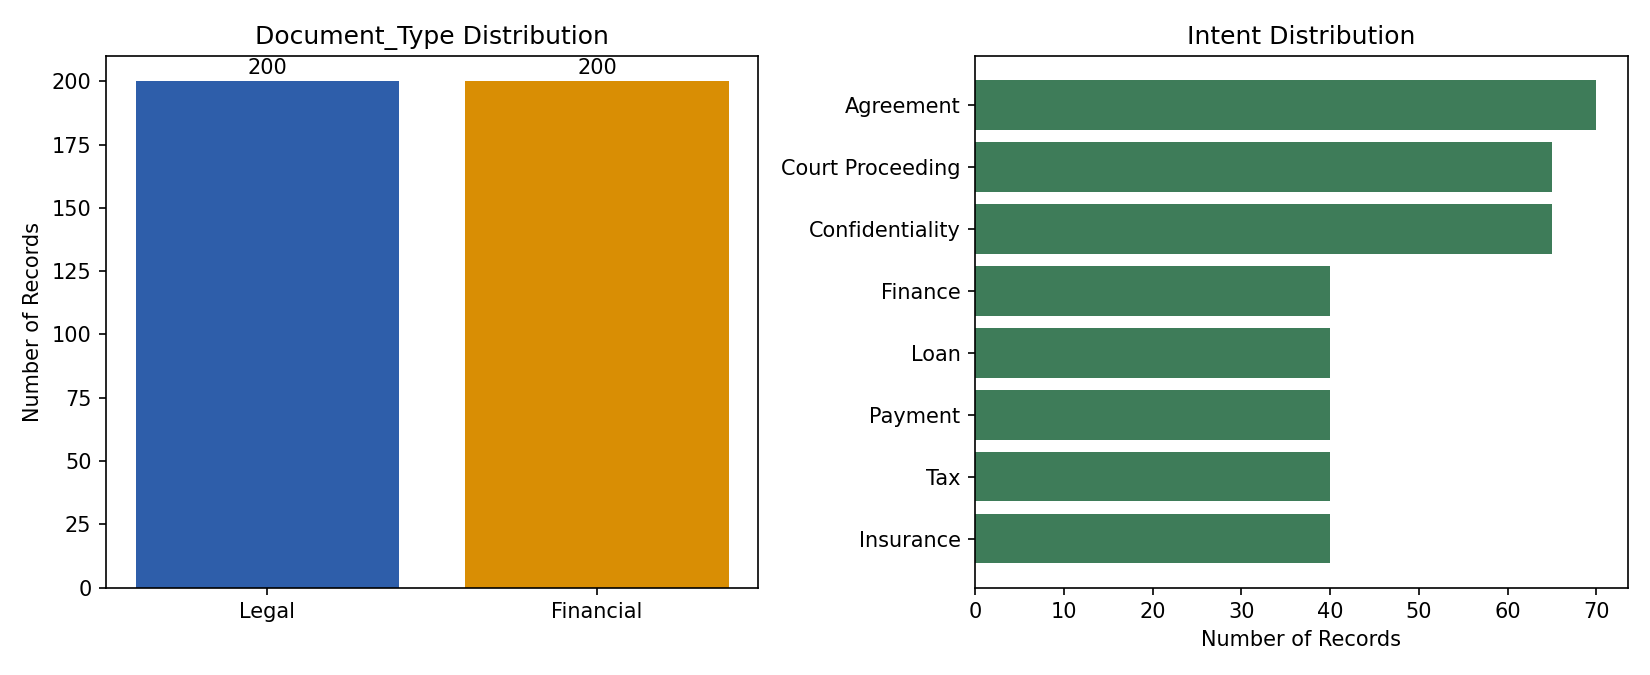
\includegraphics[width=0.95\textwidth]{figures/class_distribution.png}
\caption{Document\_Type and Intent Class Distribution}
\label{fig:classdist}
\end{figure}

\textbf{Observation:} \texttt{Document\_Type} is perfectly balanced (200 Legal / 200 Financial). \texttt{Intent} is moderately imbalanced: Agreement (70), Court Proceeding (65), and Confidentiality (65) are more frequent than the four Financial intents (40 each), reflecting the template-generation design. This imbalance should be accounted for (e.g., via class-weighted loss) when training the Intent classifier.

%%%%%%%%%%%%%%%%%%%%%%%%%%%%%%%%%%%%%%%%%%%%%%%%%%%%%%%%%%%%%%

\subsection{Vocabulary Analysis}

The dataset contains \textbf{1,196 unique whitespace-delimited tokens} across 400 records, giving a type-token ratio of approximately 1,196 / 18,764 $\approx$ 0.064, indicating a fairly repetitive, template-driven vocabulary -- expected given the synthetic generation process described in Chapter 3.

%%%%%%%%%%%%%%%%%%%%%%%%%%%%%%%%%%%%%%%%%%%%%%%%%%%%%%%%%%%%%%

\subsection{Sentence Length Distribution}

Figure~\ref{fig:sentlen} shows the histogram of record lengths measured in words.

\begin{figure}[H]
\centering
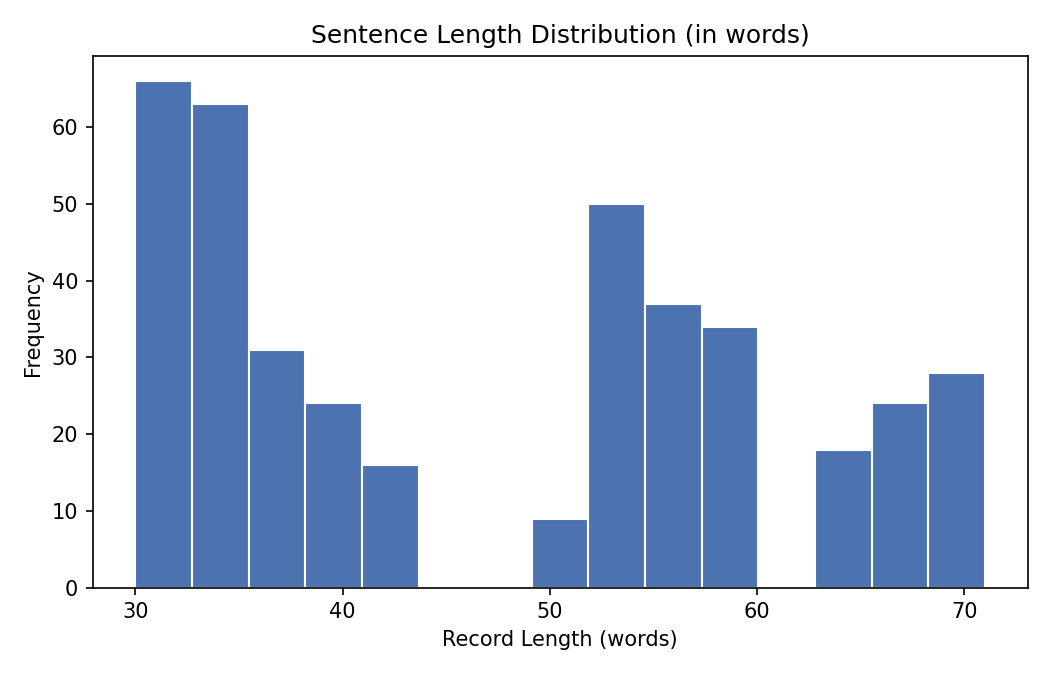
\includegraphics[width=0.75\textwidth]{figures/sentence_length_distribution.png}
\caption{Sentence Length Distribution (words per record)}
\label{fig:sentlen}
\end{figure}

\textbf{Observation:} Record lengths range from 30 to 71 words, with a mean of 46.9 words and a roughly bimodal spread reflecting the two document categories (shorter Financial notices versus longer Legal clauses). This length range is well within the input limits of standard transformer models (512 tokens), so no truncation is required.

%%%%%%%%%%%%%%%%%%%%%%%%%%%%%%%%%%%%%%%%%%%%%%%%%%%%%%%%%%%%%%

\subsection{Most Frequent Tokens}

Figure~\ref{fig:topfreq} shows the twenty most frequent tokens in the dataset.

\begin{figure}[H]
\centering
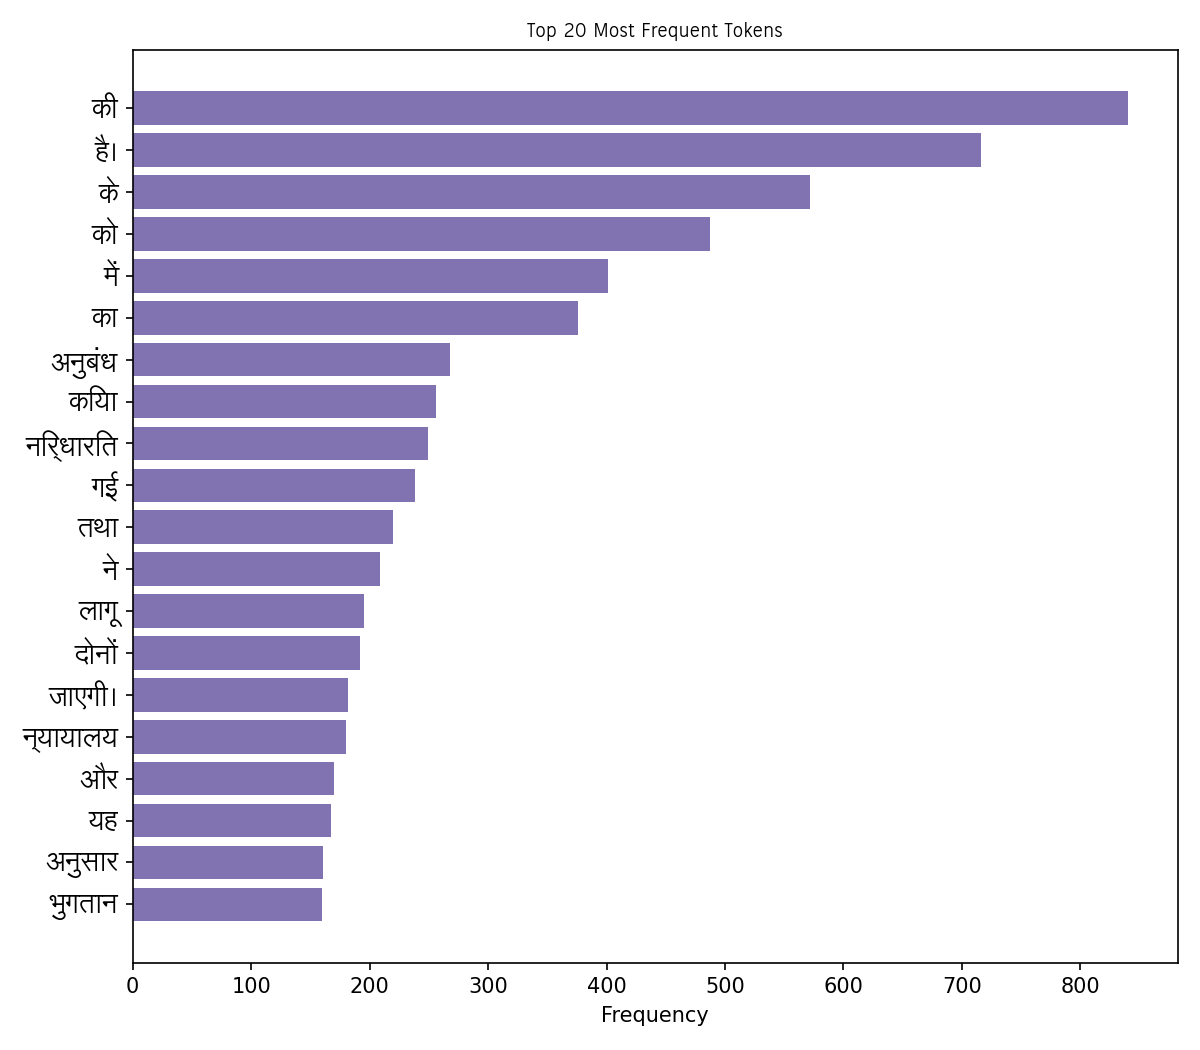
\includegraphics[width=0.7\textwidth]{figures/most_frequent_tokens.png}
\caption{Top 20 Most Frequent Tokens}
\label{fig:topfreq}
\end{figure}

\textbf{Observation:} The most frequent tokens (की, है।, के, को, में, का) are Hindi function words (postpositions and copulas), as expected. Content-bearing domain tokens such as अनुबंध (agreement/contract), निर्धारित (fixed/determined), न्यायालय (court), and भुगतान (payment) also appear among the top 20, confirming that the dataset carries clear domain signal beyond generic function words.

%%%%%%%%%%%%%%%%%%%%%%%%%%%%%%%%%%%%%%%%%%%%%%%%%%%%%%%%%%%%%%

\subsection{N-gram Analysis}

Table~\ref{tab:bigrams} presents the ten most frequent bigrams found in the dataset.

\begin{table}[H]
\centering
\caption{Top 10 Most Frequent Bigrams}
\label{tab:bigrams}
\begin{tabular}{|p{6cm}|p{3cm}|}
\hline
\textbf{Bigram} & \textbf{Frequency} \\
\hline
गई है। & 221 \\ \hline
निर्धारित की & 215 \\ \hline
की गई & 215 \\ \hline
के अनुसार & 161 \\ \hline
की जाएगी। & 156 \\ \hline
किया गया। & 136 \\ \hline
के बीच & 135 \\ \hline
दोनों पक्षों & 122 \\ \hline
किया गया & 112 \\ \hline
गया है। & 112 \\ \hline
\end{tabular}
\end{table}

\textbf{Observation:} The dominant bigrams (``निर्धारित की'', ``की गई'', ``के अनुसार'') are formal legal/financial phrasing patterns (``...is determined'', ``...as per...''), confirming the formulaic, clause-based writing style typical of legal and financial documents.

%%%%%%%%%%%%%%%%%%%%%%%%%%%%%%%%%%%%%%%%%%%%%%%%%%%%%%%%%%%%%%

\subsection{Word Cloud}

Figure~\ref{fig:wordcloud} presents a word cloud generated from the complete dataset vocabulary.

\begin{figure}[H]
\centering
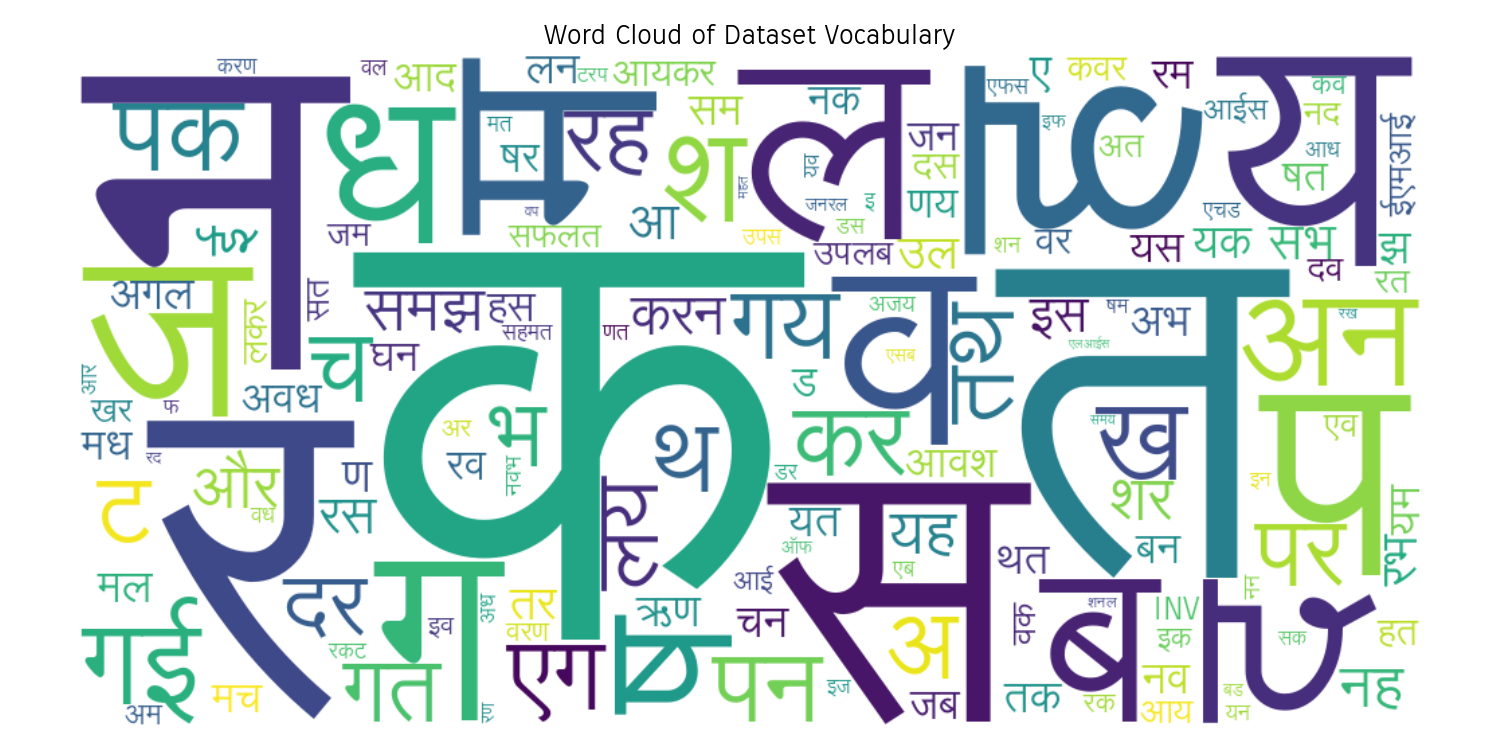
\includegraphics[width=0.85\textwidth]{figures/wordcloud.png}
\caption{Word Cloud of Dataset Vocabulary}
\label{fig:wordcloud}
\end{figure}

\textbf{Observation:} The word cloud visually reinforces the frequency analysis, with domain terms such as अनुबंध, न्यायालय, भुगतान, and निर्धारित appearing prominently alongside common Hindi function words.

%%%%%%%%%%%%%%%%%%%%%%%%%%%%%%%%%%%%%%%%%%%%%%%%%%%%%%%%%%%%%%

\subsection{Other Applicable Analyses}

Character-level and language distribution analyses were reported in Table~3.5 (Chapter 3): the dataset is 100\% Devanagari-script Hindi text with an average record length of 262 characters, and required no out-of-vocabulary (OOV) analysis since it is a closed, self-generated corpus.

%%%%%%%%%%%%%%%%%%%%%%%%%%%%%%%%%%%%%%%%%%%%%%%%%%%%%%%%%%%%%%

\section{Preprocessing Workflow}

Figure~\ref{fig:preprocessingworkflow} illustrates the complete preprocessing pipeline used in the proposed project.

\begin{figure}[H]

\centering

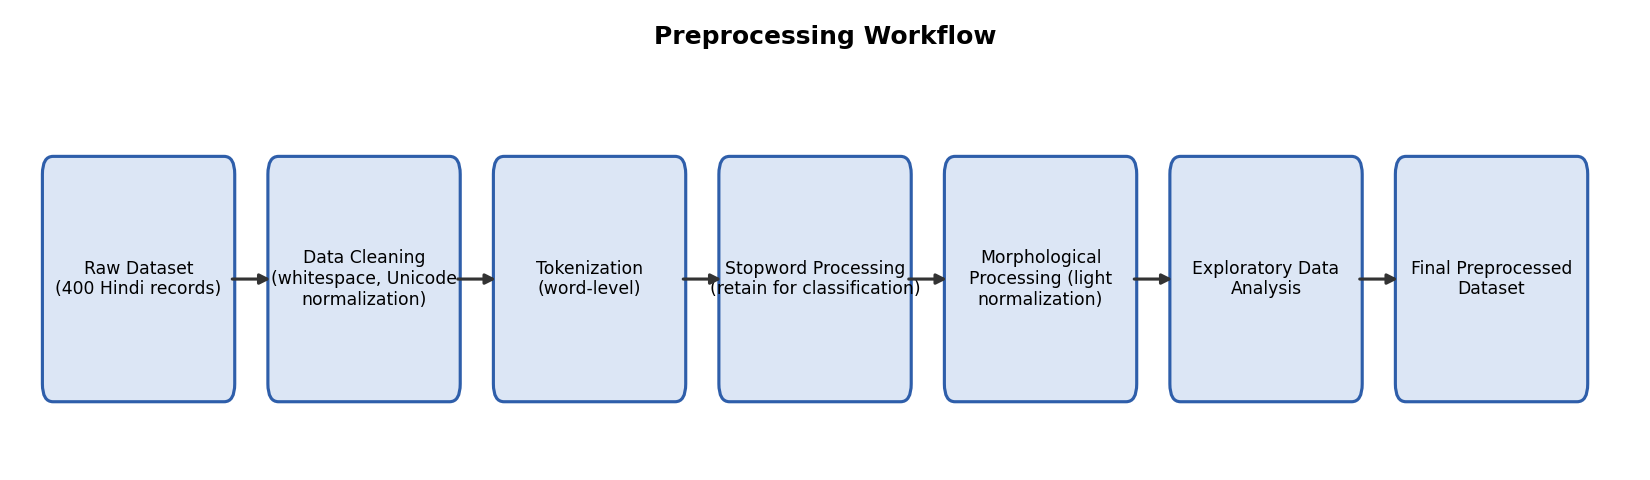
\includegraphics[width=0.95\textwidth]{figures/preprocessing_workflow.png}

\caption{Preprocessing Workflow}

\label{fig:preprocessingworkflow}

\end{figure}

The workflow illustrates:

\begin{itemize}

\item Raw Dataset (400 Hindi legal/financial records)

\item Data Cleaning (Unicode and whitespace normalization)

\item Tokenization (word-level for EDA; sub-word for model input)

\item Stopword Processing (retained for transformer pipeline; optional removal for classical ML baseline)

\item Morphological Processing (delegated to sub-word tokenizer; optional stemming for baseline)

\item Exploratory Data Analysis (class distribution, vocabulary, sentence length, n-grams)

\item Final Preprocessed Dataset (ready for feature representation and model training, Chapter 5)

\end{itemize}

\section{Preprocessing Implementation}

The implemented Node.js pipeline normalizes Unicode text, repairs whitespace and PDF line-break artefacts, preserves Devanagari combining marks, divides pages into evidence chunks, and retains each chunk's page number. Stopwords are not removed from the source evidence because legal negation and function words can change meaning. Translation is deferred until requested so that document upload remains fast and independent of a translation service.

\section{Before and After Preprocessing Analysis}

\begin{table}[H]
\centering
\caption{Representative Before and After Preprocessing Cases}
\begin{tabular}{|p{5.8cm}|p{7.2cm}|}
\hline
\textbf{Before} & \textbf{After} \\
\hline
Repeated spaces and isolated PDF line breaks & Normalized spacing with sentence continuity restored \\
\hline
Mixed Unicode forms in Hindi text & Unicode-normalized Devanagari with combining marks preserved \\
\hline
Complete document treated as one search unit & Page-linked chunks suitable for focused retrieval \\
\hline
Translation coupled to upload & Original source stored first; translation performed only on demand \\
\hline
\end{tabular}
\end{table}

The analysis shows that preprocessing improves retrieval consistency without rewriting the authoritative source text. Numeric values, dates, percentages, names, and page references remain available for answer verification.

%%%%%%%%%%%%%%%%%%%%%%%%%%%%%%%%%%%%%%%%%%%%%%%%%%%%%%%%%%%%%%

\section*{Chapter Summary}

This chapter presented the preprocessing techniques applied to the DocSaarthi dataset before model development. Data cleaning confirmed the dataset was already free of missing values, duplicates, and noise; Unicode and whitespace normalization were nonetheless applied. Tokenization, stopword processing, and morphological processing were evaluated and selectively applied based on whether the downstream model is a transformer (stopwords/morphology retained, delegated to the sub-word tokenizer) or a classical ML baseline (stopwords/stemming applied). Exploratory data analysis revealed a perfectly balanced Document\_Type split, a moderately imbalanced Intent distribution, a compact 1,196-word vocabulary reflecting the dataset's template-driven generation, and clause-based bigram patterns typical of legal/financial writing. The resulting preprocessed dataset forms the input for the feature representation and model design discussed in the next chapter.

%%%%%%%%%%%%%%%%%%%%%%%%%%%%%%%%%%%%%%%%%%%%%%%%%%%%%%%%%%%%%%
% CHAPTER 5
%%%%%%%%%%%%%%%%%%%%%%%%%%%%%%%%%%%%%%%%%%%%%%%%%%%%%%%%%%%%%%
\chapter{NLP Pipeline Design}
\label{chap:nlp_pipeline}
\markboth{Chapter \thechapter: NLP Pipeline Design}{}

%%%%%%%%%%%%%%%%%%%%%%%%%%%%%%%%%%%%%%%%%%%%%%%%%%%%%%%%%%%%%%
\section{Introduction}

This chapter presents the proposed Natural Language Processing (NLP) pipeline designed for \textit{DocSaarthi: AI Legal \& Financial Document Assistant}. It describes the overall system architecture, the end-to-end workflow, the feature representation strategy, the model selection strategy, the system requirements, and the proposed evaluation methodology. The design integrates four NLP sub-tasks -- English-to-Hindi machine translation, Legal/Financial document classification, key information extraction, and context-based question answering -- into a single bilingual pipeline, as motivated in Chapter 1 and supported by the research gaps identified in Chapter 2. The design is further grounded in the characteristics of the \textit{DocSaarthi} dataset established through the collection process in Chapter 3 and the preprocessing and exploratory analysis carried out in Chapter 4.

%%%%%%%%%%%%%%%%%%%%%%%%%%%%%%%%%%%%%%%%%%%%%%%%%%%%%%%%%%%%%%
\section{Proposed System Architecture}

The proposed system architecture illustrates the major components of the \textit{DocSaarthi} pipeline, from document acquisition to bilingual response generation.

\begin{figure}[H]
    \centering
    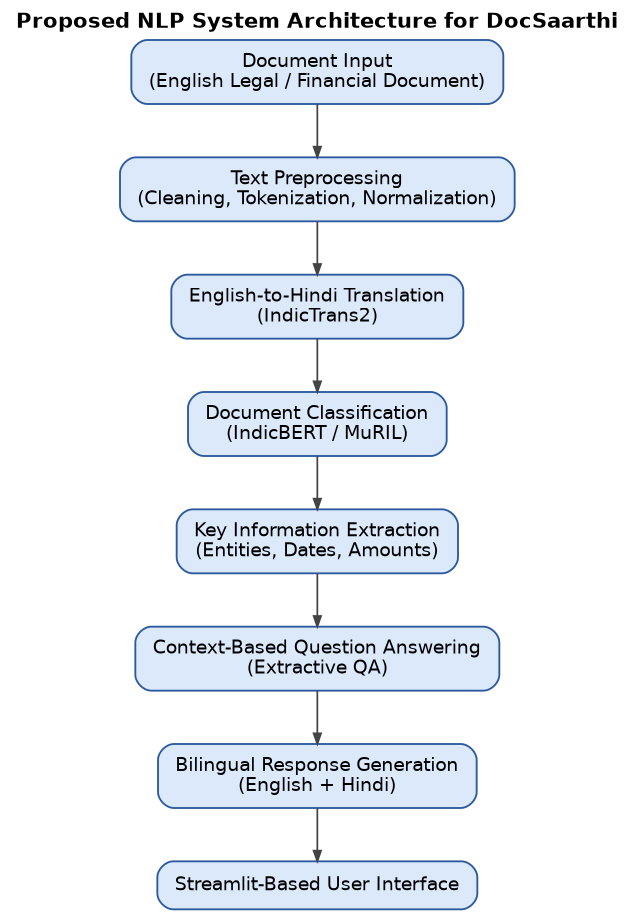
\includegraphics[width=0.95\textwidth]{figures/system_architecture.png}
    \caption{Proposed NLP System Architecture for DocSaarthi}
    \label{fig:system_architecture}
\end{figure}

The architecture consists of the following components:

\begin{enumerate}
    \item \textbf{Document Input:} A user uploads or pastes an English legal or financial document (service agreement, loan contract, insurance policy, tax notice, court proceeding excerpt, or similar) into the system.
    \item \textbf{Text Preprocessing:} The input text undergoes cleaning, tokenization, and normalization, following the preprocessing design established in Chapter 4, so that it is in a suitable form for translation and downstream modelling.
    \item \textbf{English-to-Hindi Translation:} The preprocessed document is translated from English into Hindi using a pre-trained multilingual translation model (IndicTrans2 \cite{gala2023indictrans2}), producing a Hindi version of the document alongside the original English text.
    \item \textbf{Document Classification:} The translated (or original) text is passed to a fine-tuned transformer classifier that assigns a \texttt{Document\_Type} label (Legal or Financial) and a finer-grained \texttt{Intent} label (e.g. Agreement, Loan, Tax), consistent with the label scheme of the \textit{DocSaarthi} dataset described in Chapter 3.
    \item \textbf{Key Information Extraction:} The classified document is scanned for salient fields such as party names, monetary amounts, dates, and durations, using pattern-based rules combined with contextual embeddings from the classification model.
    \item \textbf{Context-Based Question Answering:} A user may pose a natural-language question about the document; an extractive question-answering module locates the answer span within the document text, grounding every response strictly in the uploaded document.
    \item \textbf{Bilingual Response Generation:} The classification result, extracted key information, and question-answering output are rendered to the user in both English and Hindi.
    \item \textbf{Streamlit-Based User Interface:} All of the above stages are exposed to the user through a single interactive Streamlit interface, allowing document upload, translation and classification viewing, and natural-language querying without requiring the user to invoke separate tools.
\end{enumerate}

%%%%%%%%%%%%%%%%%%%%%%%%%%%%%%%%%%%%%%%%%%%%%%%%%%%%%%%%%%%%%%
\section{Workflow Diagram}

Figure~\ref{fig:workflow} illustrates the complete \textit{DocSaarthi} workflow from raw document input to the final bilingual output.

\begin{figure}[H]
    \centering
    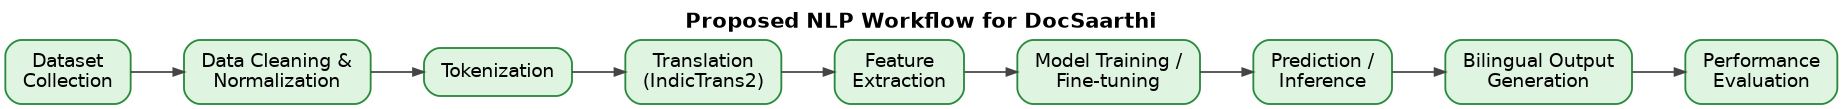
\includegraphics[width=\textwidth]{figures/workflow.png}
    \caption{Proposed NLP Workflow for DocSaarthi}
    \label{fig:workflow}
\end{figure}

The workflow consists of the following stages:

\begin{enumerate}
    \item \textbf{Dataset Collection:} Use of the 400-record, dual-labelled (\texttt{Document\_Type}, \texttt{Intent}) Hindi legal/financial dataset described in Chapter 3 for classification and extraction experiments.
    \item \textbf{Data Cleaning and Normalization:} Unicode and whitespace normalization, as applied to the dataset in Chapter 4.
    \item \textbf{Tokenization:} Word-level tokenization for exploratory analysis and sub-word tokenization for transformer model input.
    \item \textbf{Translation:} English input documents are translated into Hindi using IndicTrans2 prior to, or in parallel with, classification.
    \item \textbf{Feature Extraction:} Contextual sentence and token embeddings are obtained from the selected transformer encoder (Section~\ref{sec:feature_selected}).
    \item \textbf{Model Training / Fine-Tuning:} The classification model is fine-tuned on the labelled \textit{DocSaarthi} dataset; the question-answering module is configured for extractive answer-span prediction over document context.
    \item \textbf{Prediction / Inference:} At inference time, an uploaded document is classified, key information is extracted, and any user question is answered using the document context.
    \item \textbf{Bilingual Output Generation:} Classification labels, extracted fields, and question-answering responses are presented to the user in both English and Hindi.
    \item \textbf{Performance Evaluation:} Each stage is evaluated independently using the metrics defined in Section~\ref{sec:eval_strategy}.
\end{enumerate}

%%%%%%%%%%%%%%%%%%%%%%%%%%%%%%%%%%%%%%%%%%%%%%%%%%%%%%%%%%%%%%
\section{Feature Representation Strategy}

The effectiveness of an NLP model largely depends on how textual information is represented. Various candidate feature extraction techniques, spanning classical count-based methods and modern contextual embeddings, are considered before selecting the most appropriate representation for the bilingual, domain-specific text used in \textit{DocSaarthi}.

\subsection{Candidate Feature Representation Techniques}

\begin{longtable}{|p{4cm}|p{9cm}|}
\hline
\textbf{Technique} & \textbf{Description} \\
\hline
\endfirsthead
\hline
\textbf{Technique} & \textbf{Description} \\
\hline
\endhead
Bag of Words (BoW) & Represents documents using word occurrence counts.\\
\hline
Count Vectorizer & Converts text into frequency vectors.\\
\hline
TF-IDF & Assigns weights based on word importance.\\
\hline
Word2Vec & Dense distributed word embeddings.\\
\hline
GloVe & Global word embedding representation.\\
\hline
FastText & Uses character-level information.\\
\hline
Doc2Vec & Generates document-level embeddings.\\
\hline
BERT & Context-aware transformer embeddings.\\
\hline
RoBERTa & Optimized transformer-based representation.\\
\hline
DistilBERT & Lightweight version of BERT.\\
\hline
IndicBERT & Transformer model for Indian languages.\\
\hline
MuRIL & Multilingual representation for Indian languages.\\
\hline
XLM-R & Cross-lingual multilingual transformer.\\
\hline
\end{longtable}

\subsection{Selected Feature Representation}
\label{sec:feature_selected}

Contextual transformer-based embeddings are selected as the feature representation for \textit{DocSaarthi}, in preference to classical count-based methods (BoW, TF-IDF, Count Vectorizer) and static embeddings (Word2Vec, GloVe, FastText).

\begin{itemize}
    \item \textbf{Selected representation:} Contextual sub-word embeddings produced by an Indian-language-aware transformer encoder (IndicBERT or MuRIL \cite{khanuja2021muril}) for the Hindi classification and extraction stages, and the encoder representations internal to IndicTrans2 \cite{gala2023indictrans2} for the translation stage.
    \item \textbf{Justification:} Static embeddings and count-based representations cannot capture the polysemy and clause-level context that distinguish, for example, a loan agreement clause from a tax clause containing similar vocabulary. Transformer-based contextual embeddings, further pre-trained on Indian-language corpora, are better suited to the code-mixed, template-driven Hindi text identified during the vocabulary analysis in Chapter 4 (Section 4.4).
    \item \textbf{Expected advantages:} Strong out-of-the-box performance on Hindi through Indic-specific pre-training; sub-word tokenization that gracefully handles the limited and repetitive 1,196-word vocabulary of the dataset without excessive out-of-vocabulary issues; transferability from general-domain pre-training to the legal/financial domain through fine-tuning on a relatively small labelled set.
    \item \textbf{Computational requirements:} Fine-tuning a base-sized transformer (110--180M parameters) on the 400-record dataset is feasible on a single consumer-grade GPU or a free-tier cloud GPU runtime, in line with the hardware constraints identified in Chapter 1.
\end{itemize}

%%%%%%%%%%%%%%%%%%%%%%%%%%%%%%%%%%%%%%%%%%%%%%%%%%%%%%%%%%%%%%
\section{Model Selection Strategy}

Different machine learning and deep learning models are considered before selecting the final models for each pipeline stage.

\subsection{Candidate Models}

\begin{longtable}{|p{5cm}|p{8cm}|}
\hline
\textbf{Model} & \textbf{Description} \\
\hline
\endfirsthead
\hline
\textbf{Model} & \textbf{Description} \\
\hline
\endhead
Na\"ive Bayes & Probabilistic classifier.\\
\hline
Logistic Regression & Linear classification model.\\
\hline
Support Vector Machine & Margin-based classifier.\\
\hline
Decision Tree & Tree-based supervised learning model.\\
\hline
Random Forest & Ensemble learning approach.\\
\hline
CNN & Captures local contextual features.\\
\hline
RNN & Sequential learning model.\\
\hline
LSTM & Handles long-term dependencies.\\
\hline
Bi-LSTM & Bidirectional sequential learning.\\
\hline
GRU & Lightweight recurrent model.\\
\hline
Transformer & Attention-based architecture.\\
\hline
BERT & Bidirectional transformer encoder \cite{devlin2019bert}.\\
\hline
IndicBERT & Transformer for Indian languages.\\
\hline
MuRIL & Multilingual Indian language model.\\
\hline
T5 & Text-to-text transformer model.\\
\hline
mT5 & Multilingual T5 model.\\
\hline
IndicTrans2 & Indic-language neural machine translation model.\\
\hline
\end{longtable}

\subsection{Selected Model}

A stage-wise model selection is adopted, since \textit{DocSaarthi} is a multi-task pipeline rather than a single classification problem:

\begin{itemize}
    \item \textbf{Translation stage:} IndicTrans2 \cite{gala2023indictrans2} is selected for English-to-Hindi translation, since it is an open-source model trained specifically for all 22 scheduled Indian languages, including Hindi, and was identified in the literature review (Chapter 2) as the leading available option for this sub-task.
    \item \textbf{Classification stage:} IndicBERT or MuRIL \cite{khanuja2021muril} is selected for the \texttt{Document\_Type} (Legal/Financial) and \texttt{Intent} classification tasks, fine-tuned on the 400-record labelled dataset described in Chapter 3.
    \item \textbf{Key information extraction stage:} The same fine-tuned classification encoder is reused with a token-level (sequence-tagging) head over the extracted entity types (party names, dates, amounts, durations), avoiding the cost of training a separate large model from scratch.
    \item \textbf{Question answering stage:} An extractive question-answering formulation, using a transformer encoder with a span-prediction head over the document context, is selected in preference to a generative approach, so that every answer remains grounded in the source document text.
    \item \textbf{Selection criteria:} Availability of Hindi/Indic pre-training, open-source licensing, feasibility of fine-tuning within the hardware constraints of the micro project, and compatibility with the 400-record dataset size.
    \item \textbf{Advantages:} Reuse of pre-trained Indic language models substantially reduces the data and compute required compared to training from scratch; a shared encoder across classification and extraction reduces pipeline complexity.
    \item \textbf{Expected performance:} Given the dataset's balanced \texttt{Document\_Type} split and template-driven, low-vocabulary-diversity text (Chapter 4), high classification accuracy is expected; translation and question-answering performance is expected to be more sensitive to the fluency of the underlying pre-trained models on domain-specific legal/financial phrasing.
    \item \textbf{Possible limitations:} The 400-record dataset is small relative to typical transformer fine-tuning corpora, the four Financial intent sub-classes are comparatively under-represented (Chapter 4, Section 4.3), and none of the selected models are pre-trained specifically on Indian legal or financial text, which may limit their handling of domain-specific terminology.
\end{itemize}

%%%%%%%%%%%%%%%%%%%%%%%%%%%%%%%%%%%%%%%%%%%%%%%%%%%%%%%%%%%%%%
\section{System Requirements}

\subsection{Hardware Requirements}

\begin{table}[H]
\centering
\caption{Hardware Requirements}
\begin{tabular}{|p{5cm}|p{8cm}|}
\hline
Processor & Intel Core i5 (10th generation or later) / equivalent, quad-core, 2.5 GHz or above\\
\hline
RAM & 8 GB minimum; 16 GB recommended for transformer fine-tuning\\
\hline
Storage & At least 10 GB of free disk space for the dataset, pre-trained model checkpoints (IndicTrans2, IndicBERT/MuRIL), and supporting libraries\\
\hline
GPU (if required) & NVIDIA GPU with 6 GB or more VRAM recommended for fine-tuning; a free-tier cloud GPU runtime (e.g. Google Colab, Kaggle Notebooks) may be used as a substitute when local GPU hardware is unavailable\\
\hline
Internet Connectivity & Required for downloading pre-trained models (IndicTrans2, IndicBERT, MuRIL) and Python packages\\
\hline
\end{tabular}
\end{table}

\subsection{Software Requirements}

\begin{table}[H]
\centering
\caption{Software Requirements}
\begin{tabular}{|p{5cm}|p{8cm}|}
\hline
Operating System & Windows 10/11, Ubuntu 20.04 or later, or equivalent\\
\hline
Programming Language & Python 3.9 or later\\
\hline
IDE & Jupyter Notebook / VS Code / Google Colab\\
\hline
Libraries & pandas, NumPy, Matplotlib/Seaborn (EDA, per Chapter 4); NLTK, Indic NLP Library (preprocessing); HuggingFace Transformers, PyTorch (classification, extraction, question answering); IndicTrans2 toolkit (translation); Streamlit (user interface)\\
\hline
Version Control & Git / GitHub\\
\hline
\end{tabular}
\end{table}

%%%%%%%%%%%%%%%%%%%%%%%%%%%%%%%%%%%%%%%%%%%%%%%%%%%%%%%%%%%%%%
\section{Proposed Evaluation Strategy}
\label{sec:eval_strategy}

\subsection{Automatic Evaluation}

Since \textit{DocSaarthi} integrates four distinct NLP sub-tasks, each pipeline stage is evaluated independently using metrics appropriate to that sub-task.

\begin{longtable}{|p{5.5cm}|p{7.5cm}|}
\hline
\textbf{Pipeline Stage} & \textbf{Evaluation Metrics} \\
\hline
\endfirsthead
\hline
\textbf{Pipeline Stage} & \textbf{Evaluation Metrics} \\
\hline
\endhead
English-to-Hindi Translation & BLEU, chrF++\\
\hline
Document Classification (Legal/Financial, Intent) & Accuracy, Precision, Recall, F1-score\\
\hline
Key Information Extraction & Entity-level Precision, Recall, F1-score\\
\hline
Context-Based Question Answering & Exact Match (EM), F1-score\\
\hline
\end{longtable}

Given the moderate Intent class imbalance observed in Chapter 4 (Section 4.3), macro-averaged Precision, Recall, and F1-score are reported for the classification stage in addition to overall accuracy, so that performance on the less frequent Financial intent sub-classes is not obscured by the majority classes.

\subsection{Human Evaluation}

\begin{itemize}
    \item \textbf{Number of evaluators:} Two to three evaluators (peers and/or faculty guide), sufficient for a semester-long micro project.
    \item \textbf{Evaluation criteria:} Fluency, correctness, relevance, adequacy, coherence, and script correctness of the Hindi output.
    \item \textbf{Rating scale:} A 5-point Likert scale (1 = poor to 5 = excellent) applied per criterion.
    \item \textbf{Evaluation procedure:} A random sample of translation outputs and question-answering responses is reviewed by evaluators without access to the automatic metric scores, to avoid anchoring bias.
    \item \textbf{Agreement method (optional):} Percentage agreement between evaluators is reported where more than one evaluator rates the same sample.
\end{itemize}

\section{Proposed and Implemented Pipeline}

The initial proposal considered transformer-based translation, classification, extraction, and question answering. The implemented Review 3 prototype adopts a lighter architecture: \texttt{pdfjs-dist} for page-level PDF extraction, Unicode-aware preprocessing, lexical Legal/Financial classification, pattern-based information extraction, chunk and token-based retrieval, a 400-record Hindi intent reference set, an offline English-Hindi translation memory, and source-grounded answer generation. OpenAI-based enhancement is optional and disabled by default.

This implementation preserves the project objective while reducing infrastructure cost and hallucination risk. The uploaded PDF remains the only primary source for document facts; the intent dataset and translation memory support routing and language presentation but never replace document evidence.

Suggested evaluation criteria specific to the bilingual nature of \textit{DocSaarthi}:

\begin{itemize}
\item Fluency of the Hindi translation
\item Correctness of the classification label with respect to document content
\item Relevance of the extracted key information to the document
\item Adequacy and groundedness of question-answering responses in the source document
\item Coherence of the bilingual (English and Hindi) response presentation
\item Readability for a non-expert user
\item Script correctness (Devanagari rendering) of Hindi output
\item Cultural and domain appropriateness of legal/financial terminology used
\end{itemize}

%%%%%%%%%%%%%%%%%%%%%%%%%%%%%%%%%%%%%%%%%%%%%%%%%%%%%%%%%%%%%%
\section*{Chapter Summary}

This chapter presented the proposed NLP pipeline for \textit{DocSaarthi}, comprising a system architecture and workflow that carry an English legal or financial document through preprocessing, English-to-Hindi translation (IndicTrans2), document classification and key information extraction (IndicBERT/MuRIL), context-based question answering, and bilingual response generation, exposed to the user through a Streamlit-based interface. Contextual transformer-based embeddings were selected as the feature representation strategy, and a stage-wise model selection approach was adopted across the four pipeline sub-tasks. Hardware and software requirements were defined, and an evaluation strategy combining automatic metrics (BLEU/chrF++, Accuracy/F1, Entity-F1, EM/F1) with structured human evaluation was proposed for each stage. These design decisions provide the foundation for implementing and evaluating the proposed \textit{DocSaarthi} pipeline in subsequent project stages.

%%%%%%%%%%%%%%%%%%%%%%%%%%%%%%%%%%%%%%%%%%%%%%%%%%%%%%%%%%%%%%
% CHAPTER 6
%%%%%%%%%%%%%%%%%%%%%%%%%%%%%%%%%%%%%%%%%%%%%%%%%%%%%%%%%%%%%%

\chapter{System Implementation}
\label{chap:system_implementation}
\markboth{Chapter \thechapter: System Implementation}{}

%%%%%%%%%%%%%%%%%%%%%%%%%%%%%%%%%%%%%%%%%%%%%%%%%%%%%%%%%%%%%%
\section{Introduction}

This chapter describes the implementation of the proposed
\textbf{DocSaarthi: AI Legal \& Financial Document Assistant}.
The system is implemented as a bilingual document-intelligence
prototype that processes legal and financial PDF documents and
provides structured information to the user.

The implementation includes PDF upload and validation, text
extraction, language detection, legal/financial document
classification, key information extraction, document summarization,
bilingual retrieval, English--Hindi translation, and context-based
question answering. The system also provides page-level evidence so
that users can verify the generated information against the original
document.

The implementation was developed as a local prototype using
JavaScript and Node.js, with a 400-record Hindi intent dataset for
question-intent routing. Translation is provided through the Sarvam
translation API, while OpenAI-based answer generation is available as
an optional enhancement. The implementation focuses on maintaining the
uploaded document as the authoritative source of information.

%%%%%%%%%%%%%%%%%%%%%%%%%%%%%%%%%%%%%%%%%%%%%%%%%%%%%%%%%%%%%%
\section{Implementation Environment}

The DocSaarthi prototype was implemented using a web-based
client-server architecture. The backend handles document processing,
text extraction, classification, retrieval, translation, and answer
generation, while the frontend provides the user interface for
document upload and interaction.

\subsection{Hardware Environment}

The following hardware configuration is suitable for implementing and
testing the prototype.

\begin{table}[H]
\centering
\caption{Hardware Environment}
\begin{tabular}{|p{5cm}|p{8cm}|}
\hline
\textbf{Component} & \textbf{Configuration} \\
\hline
Processor & Intel Core i5 or equivalent processor \\
\hline
RAM & 8 GB minimum; 16 GB recommended \\
\hline
Storage & At least 10 GB free storage \\
\hline
GPU & Not mandatory for the implemented prototype \\
\hline
Internet Connectivity & Required for external translation services and optional AI services \\
\hline
\end{tabular}
\end{table}

\subsection{Software Environment}

\begin{table}[H]
\centering
\caption{Software Environment}
\begin{tabular}{|p{5cm}|p{8cm}|}
\hline
\textbf{Software / Technology} & \textbf{Purpose} \\
\hline
Operating System & Windows 10/11 or equivalent \\
\hline
Programming Language & JavaScript \\
\hline
Runtime Environment & Node.js 20 or later \\
\hline
Frontend & HTML, CSS and JavaScript \\
\hline
Backend & Node.js based server application \\
\hline
PDF Processing & pdfjs-dist \\
\hline
Translation & Sarvam Translation API \\
\hline
Optional AI Service & OpenAI API \\
\hline
Dataset Format & CSV \\
\hline
Version Control & Git / GitHub \\
\hline
\end{tabular}
\end{table}

%%%%%%%%%%%%%%%%%%%%%%%%%%%%%%%%%%%%%%%%%%%%%%%%%%%%%%%%%%%%%%
\section{Dataset Implementation}

The implemented system uses a labelled dataset containing
\textbf{400 records} for intent classification. The dataset is used
primarily for understanding and routing user queries rather than as
the evidence source for answering questions about uploaded documents.

The dataset contains Hindi-language intent examples representing
different types of user queries related to legal and financial
documents. The dataset is stored in CSV format and is loaded by the
application during execution.

The document itself remains the primary source of truth. Therefore,
information from the intent dataset is not directly used as evidence
for answering document-related questions.

\subsection{Dataset Loading}

The dataset is loaded by the application from the configured CSV
file. During initialization, the system checks whether the dataset is
available and loads the records required for intent identification.

The implementation also provides a dataset inspection utility to
check the number and distribution of records before execution.

\subsection{Dataset Usage}

The dataset is used for the following purposes:

\begin{itemize}
    \item Identifying the probable intent of a user's question.
    \item Routing questions to the appropriate document-processing
    logic.
    \item Supporting bilingual question handling.
    \item Improving the interaction between the user and the document
    assistant.
\end{itemize}

The dataset is not treated as authoritative evidence for document
answers. This separation helps prevent unrelated training examples
from being incorrectly presented as information extracted from the
uploaded document.

%%%%%%%%%%%%%%%%%%%%%%%%%%%%%%%%%%%%%%%%%%%%%%%%%%%%%%%%%%%%%%
\section{Preprocessing Implementation}

The preprocessing stage converts the extracted PDF content into a
clean and searchable textual representation. Since legal and financial
documents contain important numbers, dates, percentages, names, and
special symbols, preprocessing is performed carefully to avoid
removing meaningful information.

The implemented preprocessing pipeline consists of PDF text
extraction, Unicode normalization, line-break handling, duplicate
removal, text cleaning, tokenization, and document chunking.

\subsection{PDF Text Extraction}

The uploaded PDF is processed page by page using the
\texttt{pdfjs-dist} library. The extracted text is associated with its
corresponding page number.

This page-level representation is important because the system uses
the original page as evidence when displaying answers to the user.

\subsection{Text Cleaning}

The extracted text is cleaned before further processing. The
implementation handles unnecessary line breaks, repeated whitespace,
and common formatting inconsistencies while preserving important
information such as:

\begin{itemize}
    \item Names
    \item Dates
    \item Monetary values
    \item Percentages
    \item Legal clauses
    \item Financial terms
    \item Document identifiers
\end{itemize}

\subsection{Unicode Normalization}

Unicode normalization is applied to ensure that visually similar
characters are represented consistently. This is particularly
important for Hindi text because Devanagari characters may contain
combining marks.

The preprocessing stage therefore preserves Devanagari characters
instead of applying aggressive character removal.

\subsection{Document Chunking}

Long documents are divided into smaller text chunks before retrieval
and translation. Chunking allows the system to search relevant
sections efficiently and prevents excessively long text from being
sent to external translation or AI services.

Each chunk retains its relationship with the original document page,
allowing the final answer to provide page-level evidence.

%%%%%%%%%%%%%%%%%%%%%%%%%%%%%%%%%%%%%%%%%%%%%%%%%%%%%%%%%%%%%%
\section{Feature Representation Implementation}

The implemented prototype uses a combination of lexical and
structured textual representations rather than training a new
transformer model from scratch.

The extracted document text is represented using normalized tokens
and searchable text chunks. Token sets are used internally for
matching user queries with relevant document sections.

\subsection{Lexical Representation}

Important terms from the document and user query are normalized and
represented as token sets. These representations are used for
retrieval and matching.

For example, a query containing terms such as ``loan'', ``interest'',
``penalty'', or ``payment'' can be matched against relevant portions
of the uploaded financial document.

\subsection{Bilingual Representation}

The system supports English and Hindi interaction. A Hindi question
can be processed against English document content by using the
translation and retrieval layer.

Similarly, English queries can retrieve information from content that
has been translated or represented in Hindi.

This provides cross-language retrieval without modifying the
authoritative original document.

\subsection{Structured Information Representation}

In addition to textual chunks, the system maintains structured
information extracted from the document, including:

\begin{itemize}
    \item Dates
    \item Monetary values
    \item Percentages
    \item Important clauses
    \item Potential risk signals
    \item Document classification
    \item Page references
\end{itemize}

These representations help the system provide more useful and
verifiable responses.

%%%%%%%%%%%%%%%%%%%%%%%%%%%%%%%%%%%%%%%%%%%%%%%%%%%%%%%%%%%%%%
\section{Model Implementation}

The implementation uses a multi-stage approach rather than a single
machine learning model.

\subsection{Document Classification}

The uploaded document is classified as either \textbf{Legal} or
\textbf{Financial}. The current prototype uses document-content
analysis and heuristic/lexical signals to determine the most probable
category.

The system also provides a confidence value along with the predicted
category.

\subsection{Language Detection}

The system detects whether the uploaded document contains English,
Hindi, or mixed-language content. This information is used to
determine the appropriate processing and translation flow.

\subsection{Key Information Extraction}

The implementation identifies important information from the
document, including dates, monetary amounts, percentages, and
potentially important clauses.

Regular expressions and domain-specific lexical patterns are used for
extracting structured values.

\subsection{Question Answering}

The question-answering component follows a source-grounded approach.
The user submits a question in English or Hindi. The system searches
the indexed document chunks and retrieves the most relevant evidence.

The answer is generated only from the retrieved document content.
When sufficient evidence cannot be found, the system is designed to
return a ``not found'' response rather than inventing information.

\subsection{Translation}

English--Hindi translation is implemented using the Sarvam translation
API. Translation is treated as a separate convenience layer and does
not replace the original document.

The system supports:

\begin{itemize}
    \item English-to-Hindi translation.
    \item Hindi-to-English translation where required.
    \item Hindi summaries.
    \item Bilingual question and answer interaction.
\end{itemize}

The implementation also includes text chunking and error handling for
long translation requests.

\subsection{Optional AI Answer Generation}

OpenAI-based answer generation is implemented as an optional
enhancement. It can generate more natural responses from retrieved
document evidence.

The OpenAI component is disabled unless the required configuration and
API key are explicitly provided. A local fallback mechanism is
available when the external AI service is unavailable.

%%%%%%%%%%%%%%%%%%%%%%%%%%%%%%%%%%%%%%%%%%%%%%%%%%%%%%%%%%%%%%
\section{Training Configuration}

The current DocSaarthi prototype does not perform large-scale
transformer pretraining or fine-tuning. Instead, pretrained services
and rule-based/lexical processing are combined to create a practical
document-intelligence prototype.

The 400-record intent dataset is loaded during application execution
and used for intent routing. The document-processing pipeline operates
on the uploaded PDF at runtime.

\begin{table}[H]
\centering
\caption{Training and Processing Configuration}
\begin{tabular}{|p{5cm}|p{8cm}|}
\hline
\textbf{Parameter} & \textbf{Configuration} \\
\hline
Intent Dataset & 400 labelled records \\
\hline
Dataset Format & CSV \\
\hline
Document Processing & Runtime processing of uploaded PDFs \\
\hline
Classification & Lexical/heuristic document analysis \\
\hline
Translation Model & Sarvam hosted translation service \\
\hline
Answer Generation & Local grounded logic with optional OpenAI enhancement \\
\hline
Retrieval & Document chunk and token-based matching \\
\hline
Model Fine-tuning & Not performed in the current prototype \\
\hline
GPU Requirement & Not mandatory \\
\hline
\end{tabular}
\end{table}

This configuration was selected because the project focuses on
demonstrating an integrated multilingual document-intelligence
pipeline within the available project resources.

%%%%%%%%%%%%%%%%%%%%%%%%%%%%%%%%%%%%%%%%%%%%%%%%%%%%%%%%%%%%%%
\section{Implementation Challenges and Solutions}

During implementation, several challenges were identified due to the
complexity of legal and financial documents and the requirement for
bilingual interaction.

\begin{table}[H]
\centering
\caption{Implementation Challenges and Solutions}
\begin{tabular}{|p{5cm}|p{8cm}|}
\hline
\textbf{Challenge} & \textbf{Implemented Solution} \\
\hline
Long PDF documents & Documents are divided into smaller searchable chunks. \\
\hline
PDF line-break inconsistencies & Text normalization and line-break handling are applied. \\
\hline
Hindi Unicode handling & Unicode normalization preserves Devanagari characters and combining marks. \\
\hline
English--Hindi interaction & Cross-language retrieval and translation are implemented. \\
\hline
Large translation input & Translation requests are divided into manageable chunks. \\
\hline
Important numbers and dates & Monetary values, percentages, and dates are explicitly preserved and extracted. \\
\hline
Unsupported questions & The system returns a safe ``not found'' response when sufficient evidence is unavailable. \\
\hline
Hallucination risk & Answers are grounded in retrieved document evidence. \\
\hline
External API failure & Fallback mechanisms and error handling are implemented. \\
\hline
Document verification & Page-level citations are retained with retrieved evidence. \\
\hline
\end{tabular}
\end{table}

%%%%%%%%%%%%%%%%%%%%%%%%%%%%%%%%%%%%%%%%%%%%%%%%%%%%%%%%%%%%%%
\section{Implemented System Architecture}

The implemented architecture follows a modular document-processing
workflow. The major stages of the system are shown below.

% Temporary placeholder for the architecture figure.
% Replace this block with the actual figure once the image is available.
\begin{figure}[H]
    \centering
    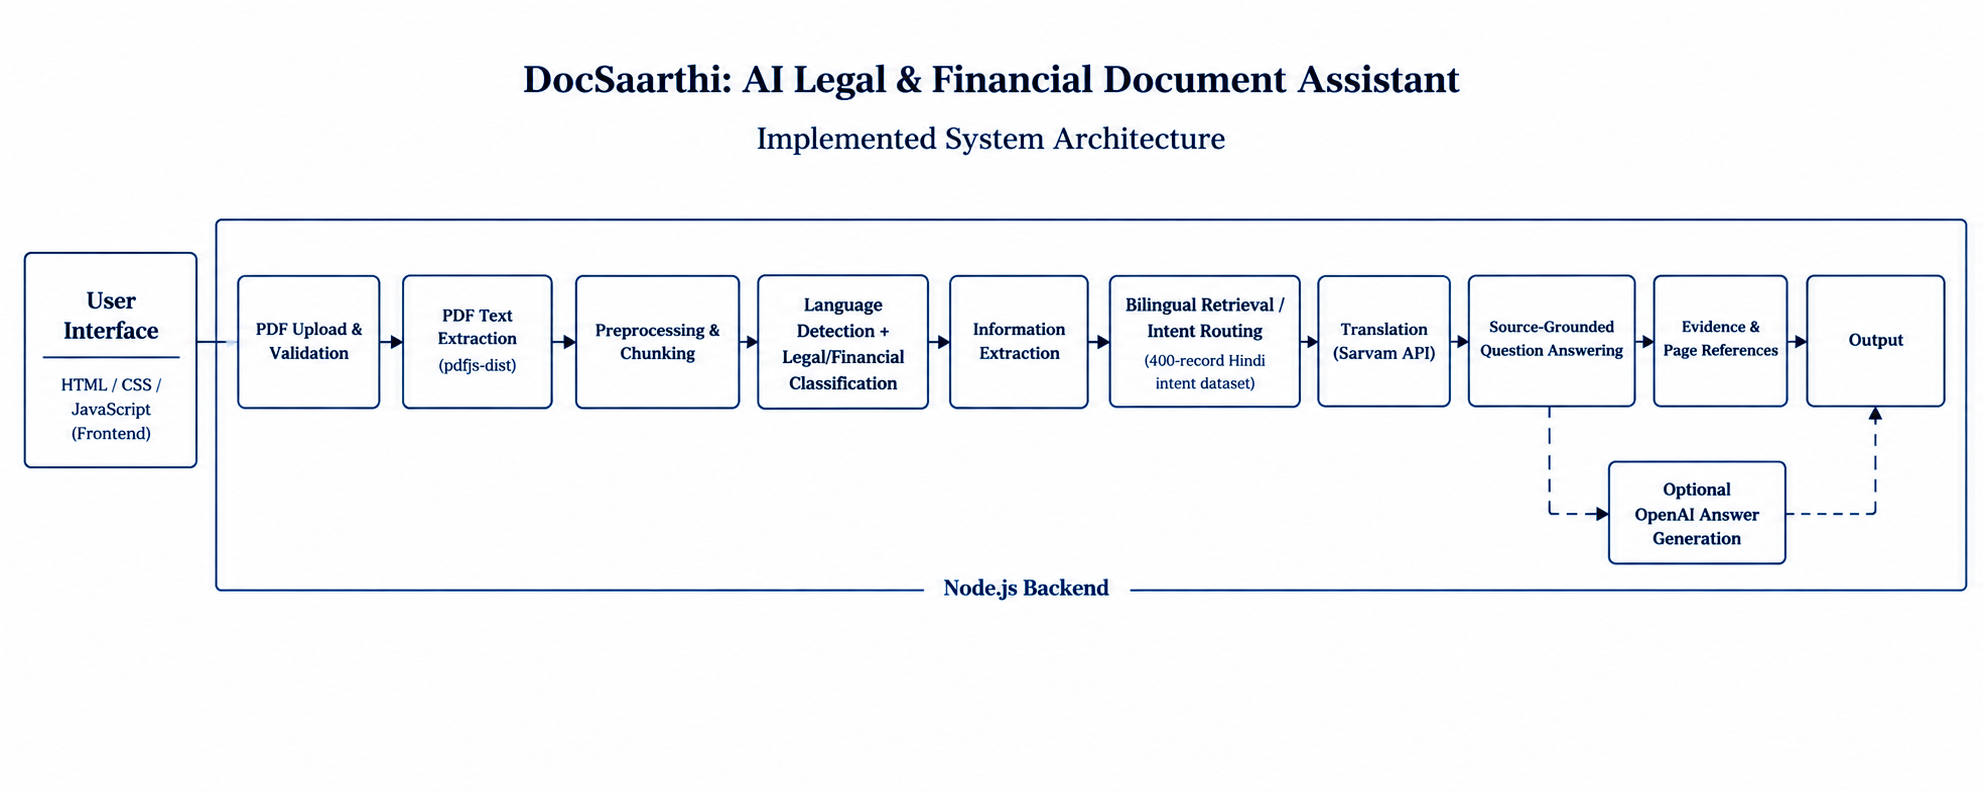
\includegraphics[width=\textwidth]{figures/implemented_system_architecture.png}
    \caption{Implemented System Architecture of DocSaarthi}
    \label{fig:implemented_architecture}
\end{figure}

The implemented system consists of the following major components:

\begin{enumerate}
    \item \textbf{User Interface:} Allows the user to upload documents,
    view results, and interact with the document assistant.

    \item \textbf{PDF Upload and Validation:} Validates the uploaded
    PDF and prepares it for processing.

    \item \textbf{PDF Text Extraction:} Extracts text from each page
    while preserving page information.

    \item \textbf{Preprocessing Module:} Performs text normalization,
    cleaning, and chunking.

    \item \textbf{Language Detection:} Identifies the language or
    language combination present in the document.

    \item \textbf{Document Classification:} Determines whether the
    document is primarily Legal or Financial.

    \item \textbf{Information Extraction:} Extracts dates, amounts,
    percentages, clauses, and potential risk signals.

    \item \textbf{Bilingual Retrieval:} Matches user questions with
    relevant document chunks in English or Hindi.

    \item \textbf{Translation Module:} Provides English--Hindi
    translation using the configured translation service.

    \item \textbf{Question Answering Module:} Generates answers based
    on retrieved document evidence.

    \item \textbf{Evidence and Citation Module:} Maintains page-level
    references so that users can verify the answer against the
    original document.

    \item \textbf{Output Module:} Displays classification, extracted
    information, summaries, translations, and question-answering
    results to the user.
\end{enumerate}

The implemented architecture follows a source-grounded design in
which the original uploaded document remains the authoritative source.
Translated content is maintained separately, and information from the
intent dataset is not used as evidence for document answers.

%%%%%%%%%%%%%%%%%%%%%%%%%%%%%%%%%%%%%%%%%%%%%%%%%%%%%%%%%%%%%%
\section*{Chapter Summary}

This chapter presented the implementation of the proposed
\textbf{DocSaarthi} system. The implementation environment, dataset
handling, preprocessing pipeline, feature representation, document
classification, information extraction, translation, and
question-answering components were described. The chapter also
discussed the processing configuration, implementation challenges and
their solutions, and the final implemented system architecture.

The implemented prototype integrates PDF processing, bilingual
interaction, document retrieval, structured information extraction,
translation, and source-grounded question answering into a single
workflow. The next chapter presents the experimental results and
evaluation of the implemented system.

%%%%%%%%%%%%%%%%%%%%%%%%%%%%%%%%%%%%%%%%%%%%%%%%%%%%%%%%%%%%%%
%%%%%%%%%%%%%%%%%%%%%%%%%%%%%%%%%%%%%%%%%%%%%%%%%%%%%%%%%%%%%%
% CHAPTER 7
%%%%%%%%%%%%%%%%%%%%%%%%%%%%%%%%%%%%%%%%%%%%%%%%%%%%%%%%%%%%%%

\chapter{Experimentation and Model Development}
\label{chap:experimentation_model_development}

\markboth{Chapter 7}{Experimentation and Model Development}

%%%%%%%%%%%%%%%%%%%%%%%%%%%%%%%%%%%%%%%%%%%%%%%%%%%%%%%%%%%%%%
\section{Introduction}

This chapter presents the experimentation and model-development
process carried out for the proposed
\textbf{DocSaarthi: AI Legal \& Financial Document Assistant}.
The objective of the experimentation stage was to evaluate different
processing strategies for document classification, information
retrieval, bilingual interaction, translation, and
source-grounded question answering.

The experiments were designed according to the implemented prototype
described in the previous chapter. Since the current implementation
does not perform large-scale transformer fine-tuning, the experiments
focus on lexical and rule-based processing, document chunk matching,
intent routing, translation, and optional AI-based answer generation.

The experimentation process was used to identify a practical
configuration that provides reliable document-based responses while
preserving important legal and financial information such as dates,
monetary values, percentages, clauses, and page references.

%%%%%%%%%%%%%%%%%%%%%%%%%%%%%%%%%%%%%%%%%%%%%%%%%%%%%%%%%%%%%%
\section{Experimental Design}

The experimental design was divided into multiple stages to evaluate
the individual components of the DocSaarthi pipeline.

The major experimental stages were:

\begin{enumerate}
    \item Preparation and inspection of the 400-record Hindi intent
    dataset.
    \item Testing of PDF text extraction and page-level text
    preservation.
    \item Evaluation of text preprocessing and document chunking.
    \item Testing of lexical query-to-document matching.
    \item Evaluation of Legal and Financial document classification.
    \item Testing of English--Hindi translation.
    \item Evaluation of source-grounded question answering.
    \item Comparison of local answer generation with optional
    AI-assisted answer generation.
    \item Evaluation of page-level evidence and unsupported-question
    handling.
\end{enumerate}

The experimental workflow is summarized below.

\begin{figure}[H]
    \centering
    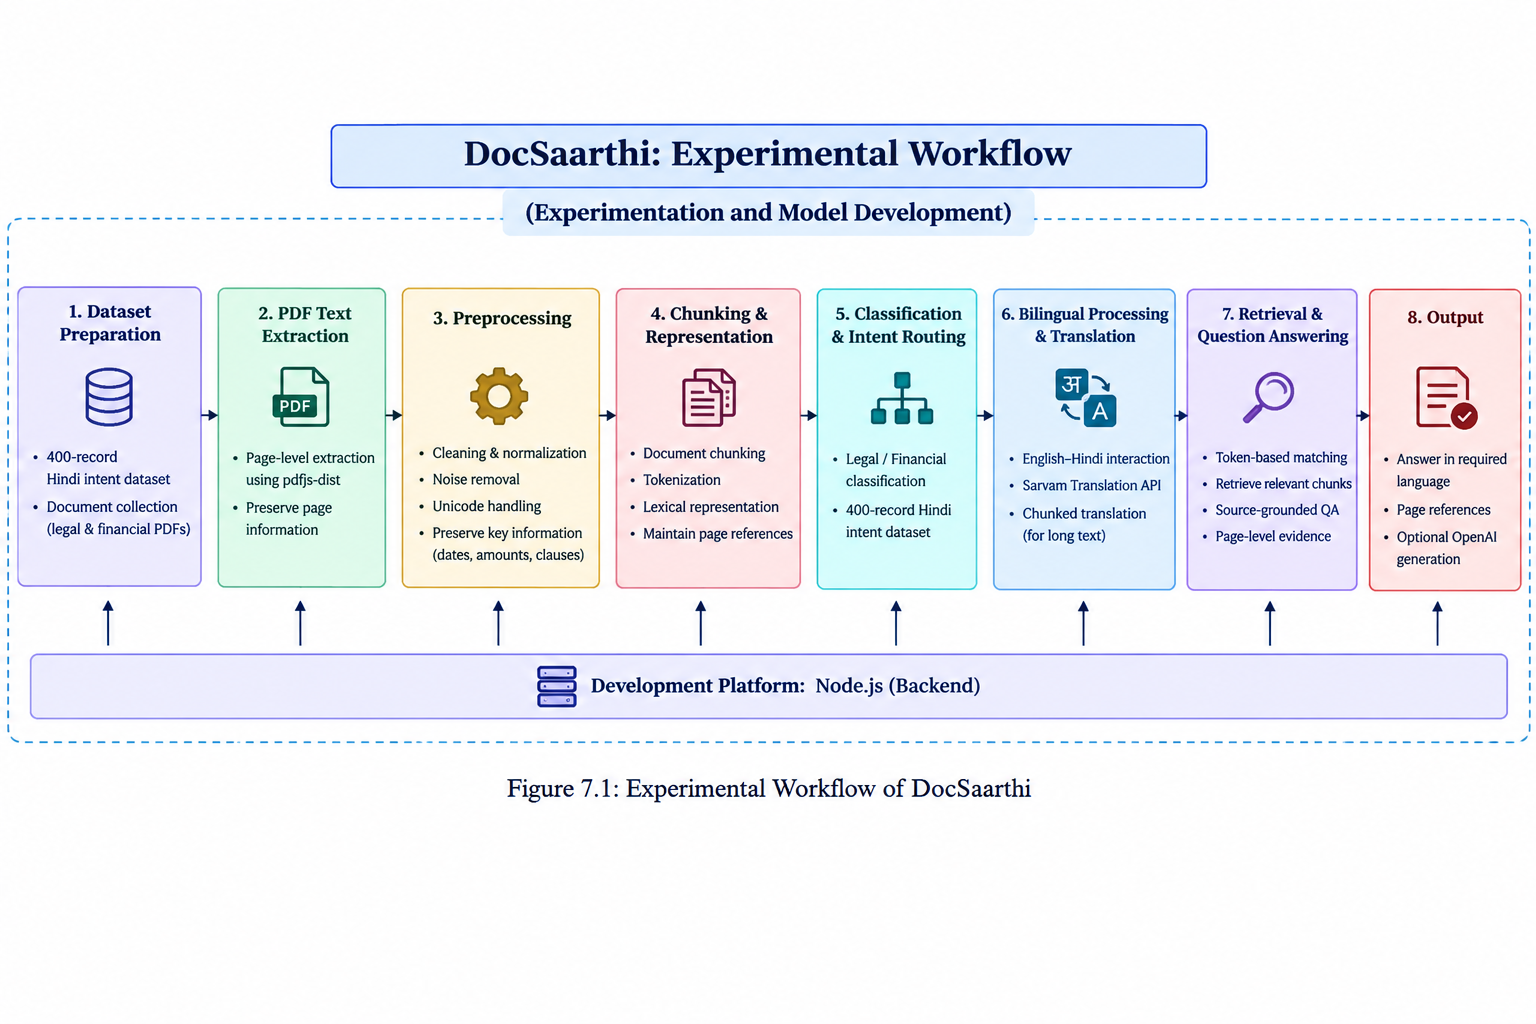
\includegraphics[width=0.95\textwidth]{figures/experimental_workflow.png}
    \caption{Experimental Workflow of DocSaarthi}
    \label{fig:experimental_workflow}
\end{figure}

The same document set was used wherever possible so that different
processing configurations could be compared under similar
conditions.

%%%%%%%%%%%%%%%%%%%%%%%%%%%%%%%%%%%%%%%%%%%%%%%%%%%%%%%%%%%%%%
\section{Baseline Model}

A baseline configuration was established to provide a reference for
evaluating the proposed document-intelligence pipeline.

The baseline approach uses direct document text processing with
basic lexical matching and limited preprocessing. User queries are
matched against the extracted document text without applying the
complete bilingual retrieval and evidence-handling workflow.

The baseline configuration consists of:

\begin{itemize}
    \item Basic PDF text extraction.
    \item Basic text cleaning.
    \item Direct keyword-based matching.
    \item Simple document category identification.
    \item Direct response generation from matched text.
\end{itemize}

The baseline provides a simple reference implementation against which
the improvements introduced by the proposed configuration can be
observed.

\begin{table}[H]
\centering
\caption{Baseline Configuration}
\begin{tabular}{|p{5cm}|p{8cm}|}
\hline
\textbf{Component} & \textbf{Baseline Configuration} \\
\hline
PDF Processing & Basic page-level text extraction \\
\hline
Preprocessing & Basic cleaning and whitespace handling \\
\hline
Representation & Keyword/token representation \\
\hline
Retrieval & Direct lexical matching \\
\hline
Classification & Basic content-based classification \\
\hline
Translation & External translation service when required \\
\hline
Question Answering & Direct response from matched content \\
\hline
Evidence & Limited page-level reference handling \\
\hline
\end{tabular}
\end{table}

The baseline experiment was useful for identifying the limitations of
simple keyword matching, especially for long documents and
cross-language questions.

%%%%%%%%%%%%%%%%%%%%%%%%%%%%%%%%%%%%%%%%%%%%%%%%%%%%%%%%%%%%%%
\section{Proposed Model}

The proposed configuration extends the baseline approach by
introducing a modular source-grounded document-processing pipeline.

The proposed system combines preprocessing, document chunking,
lexical retrieval, bilingual interaction, structured information
extraction, translation, and evidence-based question answering.

The major components of the proposed configuration are:

\begin{enumerate}
    \item PDF upload and validation.
    \item Page-level PDF text extraction.
    \item Unicode normalization and text cleaning.
    \item Document chunking.
    \item Legal/Financial document classification.
    \item Structured information extraction.
    \item Hindi intent routing using the 400-record dataset.
    \item Bilingual query processing.
    \item Token-based document retrieval.
    \item English--Hindi translation using the Sarvam API.
    \item Source-grounded question answering.
    \item Page-level evidence presentation.
    \item Optional OpenAI-based answer generation.
\end{enumerate}

The proposed configuration maintains the original document as the
authoritative source of information. The intent dataset is used for
question routing and is not treated as evidence for document answers.

\begin{table}[H]
\centering
\caption{Proposed Model Configuration}
\begin{tabular}{|p{5cm}|p{8cm}|}
\hline
\textbf{Component} & \textbf{Proposed Configuration} \\
\hline
PDF Processing & Page-level extraction using \texttt{pdfjs-dist} \\
\hline
Preprocessing & Cleaning, Unicode normalization and chunking \\
\hline
Representation & Normalized tokens and document chunks \\
\hline
Classification & Lexical/heuristic Legal-Financial classification \\
\hline
Intent Routing & 400-record Hindi intent dataset \\
\hline
Retrieval & Token and lexical document matching \\
\hline
Translation & Sarvam Translation API \\
\hline
Question Answering & Source-grounded document QA \\
\hline
Answer Enhancement & Optional OpenAI-based generation \\
\hline
Evidence & Page-level document references \\
\hline
Fallback & ``Not found'' response for insufficient evidence \\
\hline
\end{tabular}
\end{table}

%%%%%%%%%%%%%%%%%%%%%%%%%%%%%%%%%%%%%%%%%%%%%%%%%%%%%%%%%%%%%%
\section{Feature Representation Experiments}

Feature representation experiments were conducted to determine how
document and query text should be represented for effective matching.

Since the current prototype does not train a new transformer model,
the experiments focused on lexical and structured representations.

\subsection{Raw Text Representation}

In the initial experiment, extracted document text was retained as
plain text. This representation was useful for preserving the original
content but was less effective for direct matching in long documents.

Long documents contained formatting inconsistencies, repeated
whitespace, and line breaks that could reduce the effectiveness of
simple matching.

\subsection{Normalized Token Representation}

The next experiment applied text normalization and tokenization.
Important terms were converted into a consistent representation before
matching.

This representation improved the ability to identify relevant
document sections when the query and document used similar terminology.

\subsection{Chunk-Based Representation}

The document was divided into smaller searchable chunks while
retaining the original page reference.

Chunk-based representation improved retrieval because the system could
identify smaller portions of a document rather than processing the
complete document for every question.

\subsection{Structured Information Representation}

Structured information such as dates, monetary values, percentages,
clauses, and document classification was maintained separately from
the general text representation.

This representation is particularly useful for legal and financial
questions where numerical and contractual information must be
preserved accurately.

\begin{table}[H]
\centering
\caption{Feature Representation Experiments}
\begin{tabular}{|p{4cm}|p{5cm}|p{4cm}|}
\hline
\textbf{Representation} & \textbf{Purpose} & \textbf{Observation} \\
\hline
Raw Text & Preserve extracted document content & Simple but less suitable for long-document matching \\
\hline
Normalized Tokens & Improve lexical matching & More consistent query matching \\
\hline
Document Chunks & Retrieve relevant sections & Improved focused retrieval and evidence tracking \\
\hline
Structured Values & Preserve dates and numerical information & Useful for legal and financial queries \\
\hline
\end{tabular}
\end{table}

%%%%%%%%%%%%%%%%%%%%%%%%%%%%%%%%%%%%%%%%%%%%%%%%%%%%%%%%%%%%%%
\section{Model Comparison}

The baseline and proposed configurations were compared using
functional and qualitative criteria relevant to the DocSaarthi
application.

The comparison focused on retrieval quality, bilingual support,
document verification, handling of long documents, and resistance to
unsupported answers.

\begin{table}[H]
\centering
\caption{Baseline and Proposed Model Comparison}
\begin{tabular}{|p{5cm}|p{3.5cm}|p{3.5cm}|}
\hline
\textbf{Parameter} & \textbf{Baseline} & \textbf{Proposed} \\
\hline
Text Preprocessing & Basic & Normalization and cleaning \\
\hline
Document Chunking & Limited & Implemented \\
\hline
Query Matching & Direct lexical matching & Chunk and token-based matching \\
\hline
Bilingual Interaction & Limited & English--Hindi support \\
\hline
Intent Routing & Not emphasized & 400-record Hindi intent dataset \\
\hline
Information Extraction & Basic & Structured extraction \\
\hline
Translation & External translation when required & Integrated translation layer \\
\hline
Evidence Tracking & Limited & Page-level evidence \\
\hline
Unsupported Questions & May produce weak matches & ``Not found'' fallback \\
\hline
Answer Generation & Direct response & Grounded response with optional AI enhancement \\
\hline
\end{tabular}
\end{table}

The proposed configuration provides a more complete workflow for
document understanding because retrieval, translation, evidence
tracking, and answer generation are integrated into the same pipeline.

%%%%%%%%%%%%%%%%%%%%%%%%%%%%%%%%%%%%%%%%%%%%%%%%%%%%%%%%%%%%%%
\section{Hyperparameter Experimentation}

The current prototype does not perform neural network training or
transformer fine-tuning. Therefore, conventional training
hyperparameters such as learning rate, batch size, and number of
epochs are not applicable to the implemented system.

Instead, experimentation was performed on processing parameters that
affect document retrieval and response generation.

The important configurable parameters include:

\begin{itemize}
    \item Document chunk size.
    \item Amount of text overlap between chunks.
    \item Number of retrieved document chunks.
    \item Lexical matching threshold.
    \item Maximum translation text length.
    \item Query normalization rules.
    \item Answer-generation configuration.
\end{itemize}

These parameters were adjusted to achieve a balance between retrieval
coverage, response relevance, processing time, and API limitations.

\begin{table}[H]
\centering
\caption{Processing Parameter Experimentation}
\begin{tabular}{|p{5cm}|p{4cm}|p{4cm}|}
\hline
\textbf{Parameter} & \textbf{Effect of Increasing Value} & \textbf{Experimental Consideration} \\
\hline
Chunk Size & More context per retrieval unit & Very large chunks may reduce retrieval precision \\
\hline
Chunk Overlap & Better continuity between sections & Excessive overlap increases repeated content \\
\hline
Retrieved Chunks & More contextual information & Too many chunks may introduce irrelevant text \\
\hline
Matching Threshold & Stricter relevance filtering & Excessive threshold may miss valid evidence \\
\hline
Translation Chunk Length & Larger translation context & Very large inputs may exceed service limits \\
\hline
\end{tabular}
\end{table}

The final processing configuration was selected based on practical
testing with the implemented document-processing workflow.

%%%%%%%%%%%%%%%%%%%%%%%%%%%%%%%%%%%%%%%%%%%%%%%%%%%%%%%%%%%%%%
\section{Experimental Observations}

The experiments produced several important observations.

\subsection{Observation 1: Importance of Preprocessing}

Raw PDF text cannot always be used directly for reliable retrieval.
Line breaks, repeated spaces, and formatting inconsistencies can
affect lexical matching. Text normalization therefore improves the
consistency of the document representation.

\subsection{Observation 2: Importance of Chunking}

Chunking improves retrieval for long legal and financial documents.
Instead of searching the entire document as a single unit, the system
can identify smaller sections that are more closely related to the
user's question.

\subsection{Observation 3: Importance of Page References}

Maintaining page information during extraction and chunking is
important for document verification. Users can trace the generated
response back to the relevant section of the original document.

\subsection{Observation 4: Bilingual Interaction}

Translation enables users to interact with English documents using
Hindi questions and responses. However, translation is maintained as
a separate processing layer so that the original English document
remains unchanged.

\subsection{Observation 5: Source Grounding}

Restricting answers to retrieved document evidence reduces the risk of
providing information that is not present in the uploaded document.
When adequate evidence cannot be retrieved, the system can return a
``not found'' response.

\subsection{Observation 6: External Service Dependency}

The translation and optional AI answer-generation components depend on
external services. Therefore, error handling and fallback mechanisms
are required to maintain system usability when external services are
unavailable.

\subsection{Observation 7: Intent Dataset Usage}

The 400-record Hindi dataset is useful for identifying and routing
user query intents. However, it is not used as the authoritative
knowledge source for document answers.

%%%%%%%%%%%%%%%%%%%%%%%%%%%%%%%%%%%%%%%%%%%%%%%%%%%%%%%%%%%%%%
\section{Selected Model and Configuration}

Based on the experimentation, the proposed source-grounded
configuration was selected for the DocSaarthi prototype.

The selected configuration combines lexical document retrieval,
document chunking, structured information extraction, bilingual
translation, intent routing, and page-level evidence.

\begin{table}[H]
\centering
\caption{Selected Model and Configuration}
\begin{tabular}{|p{5cm}|p{8cm}|}
\hline
\textbf{Component} & \textbf{Selected Configuration} \\
\hline
Programming Language & JavaScript \\
\hline
Runtime & Node.js 20 or later \\
\hline
PDF Processing & \texttt{pdfjs-dist} \\
\hline
Text Representation & Normalized tokens and document chunks \\
\hline
Document Classification & Lexical/heuristic analysis \\
\hline
Intent Dataset & 400 labelled Hindi records \\
\hline
Retrieval & Token and lexical matching \\
\hline
Translation & Sarvam Translation API \\
\hline
Question Answering & Source-grounded document QA \\
\hline
AI Enhancement & Optional OpenAI answer generation \\
\hline
Evidence & Page-level references \\
\hline
Fine-tuning & Not performed \\
\hline
\end{tabular}
\end{table}

The selected configuration provides a practical balance between
implementation complexity, processing requirements, bilingual
functionality, and document-grounded response generation.

%%%%%%%%%%%%%%%%%%%%%%%%%%%%%%%%%%%%%%%%%%%%%%%%%%%%%%%%%%%%%%
\section{Stage 3 Readiness}

The experimentation stage prepares the DocSaarthi prototype for the
next stage of development and evaluation.

The following components are ready for further testing:

\begin{itemize}
    \item PDF upload and validation.
    \item Page-level PDF text extraction.
    \item Text preprocessing and normalization.
    \item Document chunking.
    \item Legal/Financial document classification.
    \item Structured information extraction.
    \item Hindi intent dataset integration.
    \item English--Hindi translation.
    \item Bilingual document retrieval.
    \item Source-grounded question answering.
    \item Page-level evidence presentation.
    \item Optional AI-based answer generation.
\end{itemize}

The next stage can focus on systematic evaluation of the implemented
system using representative legal and financial documents. Evaluation
can include retrieval relevance, classification correctness,
translation quality, answer correctness, evidence coverage, response
time, and handling of unsupported questions.

The system can also be extended in future experiments by introducing
trained multilingual models such as IndicBERT, MuRIL, or IndicTrans2
when sufficient computational resources and labelled training data
are available. Such models are not considered part of the current
implemented prototype.

%%%%%%%%%%%%%%%%%%%%%%%%%%%%%%%%%%%%%%%%%%%%%%%%%%%%%%%%%%%%%%
\section*{Chapter Summary}

This chapter presented the experimentation and model-development
process for the \textbf{DocSaarthi} system. The experimental design,
baseline configuration, proposed configuration, feature
representation experiments, model comparison, processing parameter
experimentation, and experimental observations were discussed.

The experiments showed the importance of preprocessing, document
chunking, lexical retrieval, bilingual interaction, structured
information extraction, and page-level evidence for building a
reliable legal and financial document assistant.

The source-grounded proposed configuration was selected as the final
prototype configuration. The system is now prepared for systematic
evaluation and further development in the next stage of the project.

%%%%%%%%%%%%%%%%%%%%%%%%%%%%%%%%%%%%%%%%%%%%%%%%%%%%%%%%%%%%%%
%%%%%%%%%%%%%%%%%%%%%%%%%%%%%%%%%%%%%%%%%%%%%%%%%%%%%%%%%%%%%%
% CHAPTER 8
%%%%%%%%%%%%%%%%%%%%%%%%%%%%%%%%%%%%%%%%%%%%%%%%%%%%%%%%%%%%%%

\chapter{Individual Technical Contribution}
\label{chap:individual_contribution}

%%%%%%%%%%%%%%%%%%%%%%%%%%%%%%%%%%%%%%%%%%%%%%%%%%%%%%%%%%%%%%
\section{Introduction}

This chapter describes the individual technical contributions made by
the two team members during the development of
\textbf{DocSaarthi: AI Legal \& Financial Document Assistant}.

The project integrates Natural Language Processing techniques for
English--Hindi translation, legal and financial document
classification, key information extraction, and bilingual question
answering. The implemented system also includes PDF processing,
document preprocessing, document chunking, retrieval, source-grounded
question answering, and page-level evidence verification.

The two team members, \textbf{Padmaja Shinde} and
\textbf{Akshata Naik}, contributed to different technical and
development activities throughout the project. Padmaja primarily
contributed to the core document-processing and NLP pipeline, while
Akshata contributed to bilingual interaction, testing, validation,
translation verification, and system-level integration.

Both members participated in debugging, testing, validation, and
technical documentation.

%%%%%%%%%%%%%%%%%%%%%%%%%%%%%%%%%%%%%%%%%%%%%%%%%%%%%%%%%%%%%%
\section{Individual Contribution Matrix}

Table~\ref{tab:individual_contribution} presents the major technical
contributions of Padmaja Shinde and Akshata Naik.

\begin{table}[H]
\centering
\caption{Individual Contribution Matrix}
\label{tab:individual_contribution}

\small
\renewcommand{\arraystretch}{1.05}
\setlength{\tabcolsep}{4pt}

\begin{tabular}{|
>{\raggedright\arraybackslash}p{3.2cm}|
>{\raggedright\arraybackslash}p{5.1cm}|
>{\raggedright\arraybackslash}p{5.1cm}|}

\hline
\textbf{Technical Area} &
\textbf{Padmaja Shinde} &
\textbf{Akshata Naik}
\\
\hline
Requirement Analysis &
Studied the project requirements and overall
DocSaarthi workflow. &
Studied user interaction requirements and
bilingual document-assistance requirements.
\\
\hline
PDF Processing &
Worked on PDF text extraction and page-level
document processing. &
Tested PDF processing and verified extracted
content and page references.
\\
\hline
Text Preprocessing &
Worked on text cleaning, normalization, and
preparation of document content. &
Validated preprocessing results and checked
preservation of important document information.
\\
\hline
Document Chunking &
Worked on document chunking for efficient
retrieval of relevant content. &
Tested chunk retrieval and relevance of
retrieved document sections.
\\
\hline
Intent Dataset &
Worked with the 400-record Hindi intent dataset
for query routing. &
Reviewed and tested Hindi intent examples and
query-routing behaviour.
\\
\hline
Bilingual Processing &
Worked on English--Hindi bilingual processing
and interaction flow. &
Tested English, Hindi, and bilingual queries
through the implemented system.
\\
\hline
Translation &
Integrated and tested the Sarvam Translation API. &
Validated English--Hindi translation results and
checked important terms and values.
\\
\hline
Information Extraction &
Worked on extraction of dates, monetary values,
percentages, important clauses, and document
information. &
Verified extracted information and checked
correctness of displayed values.
\\
\hline
Question Answering &
Worked on testing source-grounded question
answering. &
Validated generated answers against the
corresponding document evidence.
\\
\hline
Testing and Debugging &
Performed document processing, retrieval, and
integration testing. &
Performed bilingual, translation, output, and
system validation testing.
\\
\hline
Documentation &
Contributed to technical documentation and
report preparation. &
Contributed to testing records, documentation,
and presentation preparation.
\\
\hline
\end{tabular}
\end{table}

%%%%%%%%%%%%%%%%%%%%%%%%%%%%%%%%%%%%%%%%%%%%%%%%%%%%%%%%%%%%%%
\section{Individual Technical Tasks}

The following subsections describe the technical activities performed
by each team member during the development of DocSaarthi.

%%%%%%%%%%%%%%%%%%%%%%%%%%%%%%%%%%%%%%%%%%%%%%%%%%%%%%%%%%%%%%
\subsection{Padmaja Shinde}

Padmaja Shinde contributed primarily to the core document-processing
and NLP pipeline of the proposed system.

The major technical tasks performed were:

\begin{itemize}

    \item Analysed the requirements and overall workflow of the
    DocSaarthi system.

    \item Worked on PDF text extraction and page-level document
    processing.

    \item Worked on text preprocessing, cleaning, and normalization.

    \item Worked on document chunking to divide lengthy documents
    into manageable sections for retrieval.

    \item Worked with the 400-record Hindi intent dataset used for
    query routing.

    \item Contributed to English--Hindi bilingual processing.

    \item Integrated and tested the Sarvam Translation API.

    \item Worked on extraction of important document information,
    including:
    \begin{itemize}
        \item Dates
        \item Monetary values
        \item Percentages
        \item Important clauses
        \item Other relevant document information
    \end{itemize}

    \item Worked on testing source-grounded question answering.

    \item Participated in debugging and integration testing.

    \item Contributed to technical documentation and project report
    preparation.

\end{itemize}

These contributions correspond to the technical contribution
activities identified for Padmaja in the project material.

%%%%%%%%%%%%%%%%%%%%%%%%%%%%%%%%%%%%%%%%%%%%%%%%%%%%%%%%%%%%%%
\subsection{Akshata Naik}

Akshata Naik contributed primarily to bilingual interaction,
validation, testing, and system-level verification of the DocSaarthi
prototype.

The major technical tasks performed were:

\begin{itemize}

    \item Studied the user requirements and interaction flow of the
    legal and financial document assistant.

    \item Participated in testing PDF upload and document processing
    functionality.

    \item Verified extracted document text and page-level references.

    \item Tested preprocessing and document chunking results.

    \item Tested query routing using the Hindi intent dataset.

    \item Tested English, Hindi, and bilingual user queries.

    \item Participated in testing the English--Hindi bilingual
    processing workflow.

    \item Tested the Sarvam Translation API and verified the quality
    of translated output.

    \item Checked whether important information such as dates,
    monetary values, percentages, names, and document identifiers
    remained correctly represented after translation.

    \item Tested document classification results for Legal and
    Financial documents.

    \item Tested retrieval of relevant document sections for user
    queries.

    \item Validated source-grounded question-answering responses
    against the uploaded document.

    \item Verified page-level evidence associated with generated
    answers.

    \item Tested unsupported questions and verified the safe
    ``Not Found'' response.

    \item Assisted in identifying and reporting implementation
    issues during system testing.

    \item Participated in debugging and integration testing.

    \item Contributed to technical documentation and presentation
    preparation.

\end{itemize}

%%%%%%%%%%%%%%%%%%%%%%%%%%%%%%%%%%%%%%%%%%%%%%%%%%%%%%%%%%%%%%
\section{Testing and Debugging Contribution}

Testing and debugging were carried out collaboratively by both team
members to ensure that the implemented system performed correctly
across document processing, translation, retrieval, and
question-answering tasks.

%%%%%%%%%%%%%%%%%%%%%%%%%%%%%%%%%%%%%%%%%%%%%%%%%%%%%%%%%%%%%%
\subsection{Padmaja Shinde}

Padmaja contributed to testing and debugging of the core NLP and
document-processing components.

The testing activities included:

\begin{itemize}

    \item PDF text extraction testing.

    \item Text preprocessing and normalization testing.

    \item Document chunking testing.

    \item Document classification testing.

    \item Information extraction testing.

    \item Retrieval testing.

    \item Translation API integration testing.

    \item Source-grounded question-answering testing.

    \item Backend integration testing.

\end{itemize}

Padmaja also participated in identifying processing errors and
verifying corrections after debugging.

%%%%%%%%%%%%%%%%%%%%%%%%%%%%%%%%%%%%%%%%%%%%%%%%%%%%%%%%%%%%%%
\subsection{Akshata Naik}

Akshata contributed mainly to system-level and user-oriented testing.

The testing activities included:

\begin{itemize}

    \item Testing English and Hindi queries.

    \item Testing bilingual interaction.

    \item Testing query routing and intent handling.

    \item Testing translation output.

    \item Verifying important values after translation.

    \item Testing retrieval relevance.

    \item Checking source-grounded answers against document content.

    \item Verifying page-level evidence.

    \item Testing unsupported questions.

    \item Identifying unexpected outputs during system execution.

\end{itemize}

These testing activities support the project requirement that the
system provide bilingual responses and evidence that can be verified
against the original document.

%%%%%%%%%%%%%%%%%%%%%%%%%%%%%%%%%%%%%%%%%%%%%%%%%%%%%%%%%%%%%%
\subsection{Joint Testing and Debugging}

Both members jointly participated in end-to-end system testing.

The joint testing process included:

\begin{enumerate}

    \item Uploading legal and financial PDF documents.

    \item Checking successful PDF text extraction.

    \item Verifying preprocessing and chunking.

    \item Testing Legal and Financial classification.

    \item Checking extraction of dates, monetary values, percentages,
    and important clauses.

    \item Testing English and Hindi queries.

    \item Testing translation.

    \item Testing retrieval of relevant document chunks.

    \item Verifying source-grounded answers.

    \item Checking page-level evidence.

    \item Testing unsupported questions.

    \item Re-testing the system after debugging.

\end{enumerate}

%%%%%%%%%%%%%%%%%%%%%%%%%%%%%%%%%%%%%%%%%%%%%%%%%%%%%%%%%%%%%%
\section{Problems Encountered and Solutions}

Several technical challenges were encountered during the
implementation of DocSaarthi. The major problems and the
corresponding solutions are presented in Table~\ref{tab:problems}.

\begin{table}[H]
\centering
\caption{Problems Encountered and Implemented Solutions}
\label{tab:problems}

\renewcommand{\arraystretch}{1.25}
\setlength{\tabcolsep}{4pt}

\begin{tabular}{|
>{\raggedright\arraybackslash}p{4.2cm}|
>{\raggedright\arraybackslash}p{8.8cm}|}

\hline
\textbf{Problem} &
\textbf{Solution}
\\
\hline
Long PDF documents &
Documents were divided into smaller chunks to make retrieval and
processing more manageable.
\\
\hline
PDF text formatting issues &
Text cleaning, normalization, and line-break handling were applied
during preprocessing.
\\
\hline
Hindi Unicode handling &
Unicode normalization was used while preserving Devanagari
characters.
\\
\hline
Bilingual interaction &
English--Hindi translation and bilingual retrieval were incorporated
into the processing workflow.
\\
\hline
Long translation requests &
Large text inputs were divided into smaller translation chunks.
\\
\hline
Important numerical information &
Dates, monetary values, percentages, and identifiers were preserved
during processing.
\\
\hline
Irrelevant retrieval &
Normalized lexical and token-based matching was used to retrieve
relevant document sections.
\\
\hline
Unsupported questions &
The system provides a safe ``Not Found'' response when sufficient
evidence is unavailable.
\\
\hline
Hallucination risk &
Question answering is grounded in retrieved document evidence.
\\
\hline
External API dependency &
Error handling and fallback mechanisms were incorporated for
external services.
\\
\hline
Document verification &
Page-level references were retained so that users could verify the
generated information.
\\
\hline
\end{tabular}
\end{table}

%%%%%%%%%%%%%%%%%%%%%%%%%%%%%%%%%%%%%%%%%%%%%%%%%%%%%%%%%%%%%%
\section{Skill Acquisition and Technology Adoption}

The development of DocSaarthi provided both team members with
practical experience in Natural Language Processing, document
intelligence, bilingual processing, API integration, testing, and
debugging.

%%%%%%%%%%%%%%%%%%%%%%%%%%%%%%%%%%%%%%%%%%%%%%%%%%%%%%%%%%%%%%
\subsection{Padmaja Shinde}

The major technical skills acquired and strengthened by Padmaja
include:

\begin{itemize}

    \item PDF document processing.

    \item Page-level text extraction.

    \item Text preprocessing and normalization.

    \item Document chunking.

    \item Lexical document retrieval.

    \item Structured information extraction.

    \item Bilingual English--Hindi processing.

    \item Translation API integration.

    \item Source-grounded question answering.

    \item Backend integration and debugging.

    \item Technical documentation and report preparation.

\end{itemize}

%%%%%%%%%%%%%%%%%%%%%%%%%%%%%%%%%%%%%%%%%%%%%%%%%%%%%%%%%%%%%%
\subsection{Akshata Naik}

The major technical skills acquired and strengthened by Akshata
include:

\begin{itemize}

    \item Understanding of NLP-based document processing.

    \item Working with a Hindi intent dataset.

    \item Bilingual English--Hindi interaction.

    \item Translation API testing.

    \item Document classification validation.

    \item Retrieval and question-answering validation.

    \item Verification of extracted legal and financial information.

    \item Functional testing and debugging.

    \item System integration testing.

    \item Technical documentation and presentation preparation.

\end{itemize}

%%%%%%%%%%%%%%%%%%%%%%%%%%%%%%%%%%%%%%%%%%%%%%%%%%%%%%%%%%%%%%
\subsection{Technology Adoption}

The major technologies used during the implementation of DocSaarthi
are summarized below.

\begin{table}[H]
\centering
\caption{Technology Adoption}
\label{tab:technology_adoption}

\renewcommand{\arraystretch}{1.2}

\begin{tabular}{|p{4cm}|p{9cm}|}
\hline
\textbf{Technology} & \textbf{Application}
\\
\hline
HTML, CSS and JavaScript &
Frontend interface and user interaction.
\\
\hline
Node.js &
Backend runtime and application processing.
\\
\hline
pdfjs-dist &
PDF text extraction and page-level processing.
\\
\hline
400-record Hindi Dataset &
Intent identification and query routing.
\\
\hline
Sarvam Translation API &
English--Hindi and Hindi--English translation.
\\
\hline
Lexical / Token Matching &
Document retrieval and query matching.
\\
\hline
OpenAI API &
Optional AI-assisted answer generation.
\\
\hline
Git / GitHub &
Version control and project development.
\\
\hline
\end{tabular}
\end{table}

The project material identifies Node.js, HTML/CSS/JavaScript,
pdfjs-dist, the 400 Hindi intent records, Sarvam Translation API,
lexical/token-based retrieval, and optional OpenAI integration as the
main implementation technologies.

%%%%%%%%%%%%%%%%%%%%%%%%%%%%%%%%%%%%%%%%%%%%%%%%%%%%%%%%%%%%%%
\section{Individual Contribution Evidence}

The individual contribution of both members can be demonstrated
through the technical implementation, testing activities, system
outputs, and project documentation.

%%%%%%%%%%%%%%%%%%%%%%%%%%%%%%%%%%%%%%%%%%%%%%%%%%%%%%%%%%%%%%
\subsection{Evidence for Padmaja Shinde}

The following activities provide evidence of Padmaja's technical
contribution:

\begin{itemize}

    \item Requirement analysis and understanding of the DocSaarthi
    workflow.

    \item PDF text extraction and page-level processing.

    \item Text preprocessing and normalization.

    \item Document chunking.

    \item Integration of the 400-record Hindi intent dataset.

    \item English--Hindi bilingual processing.

    \item Sarvam Translation API integration and testing.

    \item Extraction of dates, monetary values, percentages, and
    important clauses.

    \item Testing of source-grounded question answering.

    \item Debugging and integration testing.

    \item Technical documentation and report preparation.

\end{itemize}

These activities are explicitly listed in the project's individual
contribution material.

%%%%%%%%%%%%%%%%%%%%%%%%%%%%%%%%%%%%%%%%%%%%%%%%%%%%%%%%%%%%%%
\subsection{Evidence for Akshata Naik}

The following activities provide evidence of Akshata's contribution
to the development and validation of the system:

\begin{itemize}

    \item Testing of document upload and PDF processing.

    \item Validation of extracted document content.

    \item Testing of preprocessing and document chunking.

    \item Testing of the Hindi intent dataset and query routing.

    \item Testing English, Hindi, and bilingual queries.

    \item Translation API testing and output verification.

    \item Validation of extracted dates, monetary values, percentages,
    and important clauses.

    \item Testing of Legal and Financial document classification.

    \item Retrieval relevance testing.

    \item Source-grounded question-answering validation.

    \item Page-level evidence verification.

    \item Unsupported-question testing.

    \item Debugging and integration testing.

    \item Technical documentation and presentation support.

\end{itemize}

%%%%%%%%%%%%%%%%%%%%%%%%%%%%%%%%%%%%%%%%%%%%%%%%%%%%%%%%%%%%%%
\subsection{Project Artifacts as Evidence}

The following project artifacts can be used to demonstrate the
technical contributions of both members:

\begin{itemize}

    \item Source-code files.

    \item Git/GitHub repository and commit history.

    \item Hindi intent dataset.

    \item PDF processing implementation.

    \item Translation API integration.

    \item Testing outputs.

    \item Screenshots of the implemented system.

    \item Classification and information extraction results.

    \item Question-answering results.

    \item Technical documentation.

    \item Project presentation and demonstration.

\end{itemize}

The project presentation also records the team's implementation
technologies, including Node.js, pdfjs-dist, the 400-record Hindi
dataset, Sarvam Translation API, lexical/token-based retrieval, and
optional OpenAI integration.

%%%%%%%%%%%%%%%%%%%%%%%%%%%%%%%%%%%%%%%%%%%%%%%%%%%%%%%%%%%%%%
\section*{Chapter Summary}

This chapter presented the individual technical contributions of
\textbf{Padmaja Shinde} and \textbf{Akshata Naik} in the development
of DocSaarthi.

Padmaja Shinde primarily contributed to the core document-processing
and NLP pipeline, including PDF text extraction, preprocessing,
document chunking, intent dataset integration, bilingual processing,
translation integration, information extraction, source-grounded
question answering, debugging, and technical documentation.

Akshata Naik primarily contributed to system validation, bilingual
interaction testing, translation verification, intent and query
routing validation, document classification testing, retrieval
verification, question-answering validation, debugging, and
documentation.

Both members contributed to the integration, testing, debugging, and
validation of the complete DocSaarthi system.

The contribution of Padmaja is directly documented in the project
material, including requirement analysis, PDF processing,
preprocessing, document chunking, intent dataset integration,
bilingual processing, Sarvam integration, information extraction,
question-answering testing, debugging, and documentation.


The combined contributions supported the implementation and
validation of a bilingual, source-grounded legal and financial
document assistant. The project architecture integrates document
processing, classification, information extraction, bilingual
retrieval, translation, question answering, and page-level evidence
into a single workflow.

%%%%%%%%%%%%%%%%%%%%%%%%%%%%%%%%%%%%%%%%%%%%%%%%%%%%%%%%%%%%%%
\chapter{Model Evaluation and Validation}
\label{chap:model_evaluation}

\section{Introduction}
This chapter evaluates the implemented DocSaarthi prototype using repeatable automated tests and a labelled bilingual PDF holdout. The purpose is to verify domain classification, language detection, cross-language retrieval, translation fidelity, source grounding, and safe abstention.

\section{Evaluation Methodology}
Three complementary checks were used: 18 Node.js regression tests, an eight-document labelled holdout containing four Legal and four Financial PDFs in English and Hindi, and manual inspection of representative answers and citations. The holdout is synthetic and deliberately small; therefore, its scores demonstrate prototype correctness on the controlled benchmark and are not presented as production accuracy.

\section{Evaluation Metrics}
Classification is reported using accuracy, per-class precision, recall, F1-score, macro-F1, and a confusion matrix. Language detection is reported using accuracy. Retrieval and answer generation are validated through expected evidence matching, page-number preservation, value preservation, and abstention assertions.

\section{Quantitative Evaluation}
All 18 automated tests passed. The labelled holdout produced eight correct document-domain predictions and eight correct language predictions.

\begin{table}[H]
\centering
\caption{Review 3 Quantitative Results}
\begin{tabular}{|p{7cm}|p{5cm}|}
\hline
\textbf{Measure} & \textbf{Result} \\
\hline
Automated regression tests & 18/18 passed \\
\hline
Document classification accuracy & 100\% (8/8) \\
\hline
Macro-averaged F1-score & 1.00 \\
\hline
Legal precision / recall / F1 & 1.00 / 1.00 / 1.00 \\
\hline
Financial precision / recall / F1 & 1.00 / 1.00 / 1.00 \\
\hline
Language detection accuracy & 100\% (8/8) \\
\hline
\end{tabular}
\end{table}

\section{Model Performance}
The rule-based classifier correctly separated all four Legal and four Financial samples. Displayed confidence values ranged from 0.82 to 0.84. These confidence values are bounded interface indicators rather than calibrated probabilities.

\section{Comparative Evaluation}
Compared with the earlier direct keyword baseline, the implemented pipeline adds page-linked chunks, bilingual query support, value-preserving translation checks, explicit grounding, and an abstention path. The comparison is functional because a sufficiently large real-world benchmark for statistically significant model comparison is not yet available.

\section{Class-wise / Category-wise Evaluation}
\begin{table}[H]
\centering
\caption{Confusion Matrix for the Eight-Document Holdout}
\begin{tabular}{|p{4cm}|c|c|}
\hline
\textbf{Actual Class} & \textbf{Predicted Legal} & \textbf{Predicted Financial} \\
\hline
Legal & 4 & 0 \\
\hline
Financial & 0 & 4 \\
\hline
\end{tabular}
\end{table}

\section{Human Evaluation (where applicable)}
The two team members manually verified representative bilingual answers against the corresponding source excerpt and page number during development. A formal blinded study with external evaluators and Likert-scale ratings has not yet been completed; it is retained as future work to avoid overstating evidence.

\section{Validation Results}
Validation confirmed English-to-Hindi and Hindi-to-English retrieval, preservation of rupee amounts, percentages, dates, and names, safe rejection of Hinglish output, handling of PDF line breaks, preservation of Devanagari combining marks, and abstention for unsupported questions such as a missing PAN number.

\section*{Chapter Summary}
The controlled Review 3 benchmark and regression suite validate the implemented prototype. The results are encouraging, but broader real-document and human evaluation is required before deployment claims can be made.

\chapter{Error Analysis and Model Improvement}
\label{chap:error_analysis}

\section{Introduction}
Error analysis was used to convert observed risks into regression tests and safeguards. Particular attention was given to unsupported answers, bilingual retrieval failures, translation corruption, PDF formatting artefacts, and misclassification.

\section{Error Analysis Methodology}
Each failure mode was reproduced with a minimal document and query. The expected source excerpt, output language, preserved values, page reference, or abstention behavior was then encoded as an automated assertion. A correction was accepted only after the original case and the full suite passed.

\section{Error Categories}
The principal categories were language and answer ordering, Legal/Financial classification, cross-language retrieval and grounding, translation fidelity, PDF extraction and processing, and Unicode robustness.

\section{Representative Error Cases}
\begin{longtable}{|p{3.8cm}|p{4.8cm}|p{5cm}|}
\hline
\textbf{Case} & \textbf{Risk} & \textbf{Implemented Response} \\
\hline
Unsupported PAN question & Fabricated identifier & Return a grounded ``not found'' answer with no citation \\
\hline
Hindi query on English PDF & No relevant cross-language match & Expand bilingual intent and terminology signals before retrieval \\
\hline
PDF line break inside sentence & Evidence split across chunks & Repair line breaks before sentence and chunk processing \\
\hline
Hinglish translation & Reduced readability and altered meaning & Reject invalid output using script and preservation checks \\
\hline
Amounts, dates, or percentages changed & Financial meaning corrupted & Validate protected values against the source \\
\hline
External translation failure & Upload or analysis blocked & Defer translation and retain the original source result \\
\hline
\end{longtable}

\section{Error Distribution}
The following table describes regression-test coverage, not production error frequency. Each of the 18 tests is assigned to its primary risk category.

\begin{table}[H]
\centering
\caption{Distribution of Automated Validation Coverage}
\begin{tabular}{|p{7cm}|c|c|}
\hline
\textbf{Primary Category} & \textbf{Tests} & \textbf{Share} \\
\hline
Language and answer ordering & 2 & 11.1\% \\
\hline
Classification and confidence & 2 & 11.1\% \\
\hline
Retrieval, grounding, and abstention & 5 & 27.8\% \\
\hline
Translation fidelity and value preservation & 6 & 33.3\% \\
\hline
PDF extraction and processing & 2 & 11.1\% \\
\hline
Unicode robustness & 1 & 5.6\% \\
\hline
\textbf{Total} & \textbf{18} & \textbf{100\%} \\
\hline
\end{tabular}
\end{table}

\section{Analysis of Error Causes}
The dominant causes are vocabulary mismatch between languages, unreliable layout in extracted PDFs, preservation-sensitive financial values, insufficient evidence, and dependency failure. These causes are architectural rather than a single trainable-model problem, so they require layered validation and fallback behavior.

\section{Model Improvement}
Improvements include Unicode normalization, line-break repair, page-linked chunking, bilingual retrieval signals, protected-value validation, on-demand translation, source-only answer grounding, and explicit abstention. Classification confidence is constrained to a narrow range to avoid presenting an uncalibrated score as certainty.

\section{Before and After Improvement}
\begin{table}[H]
\centering
\caption{Before and After Improvement}
\begin{tabular}{|p{5.8cm}|p{7.2cm}|}
\hline
\textbf{Before} & \textbf{After} \\
\hline
Weak match could be returned for missing facts & Unsupported questions abstain and expose no false source \\
\hline
Translation coupled to document processing & Upload remains usable even if translation fails \\
\hline
Line breaks could fragment evidence & Sentence continuity is restored before chunking \\
\hline
Mixed-language output could pass through & Hindi output is checked for natural script usage \\
\hline
Critical values could drift in translation & Names, dates, amounts, and percentages are verified \\
\hline
\end{tabular}
\end{table}

\section{Discussion of Improvement}
The final suite passing 18/18 confirms that the selected safeguards work for the encoded cases. It does not prove completeness: OCR errors, adversarial documents, unfamiliar terminology, and large-scale latency remain open evaluation areas.

\section*{Chapter Summary}
The improvement process prioritized trustworthiness and traceability. Every material safeguard is connected to a repeatable test, while unresolved limitations are stated explicitly.

\chapter{Final System and Results}
\label{chap:final_system}

\section{Introduction}
The final Review 3 prototype is a bilingual legal and financial document assistant that accepts text-based PDFs, extracts and analyses their content, and answers questions using traceable source evidence.

\section{Final System Architecture}
The browser interface communicates with a Node.js and Express backend. The backend coordinates PDF extraction, language detection, classification, information extraction, chunking, retrieval, translation, and grounded answer generation. In-memory storage is used in the prototype.

\begin{figure}[H]
\centering
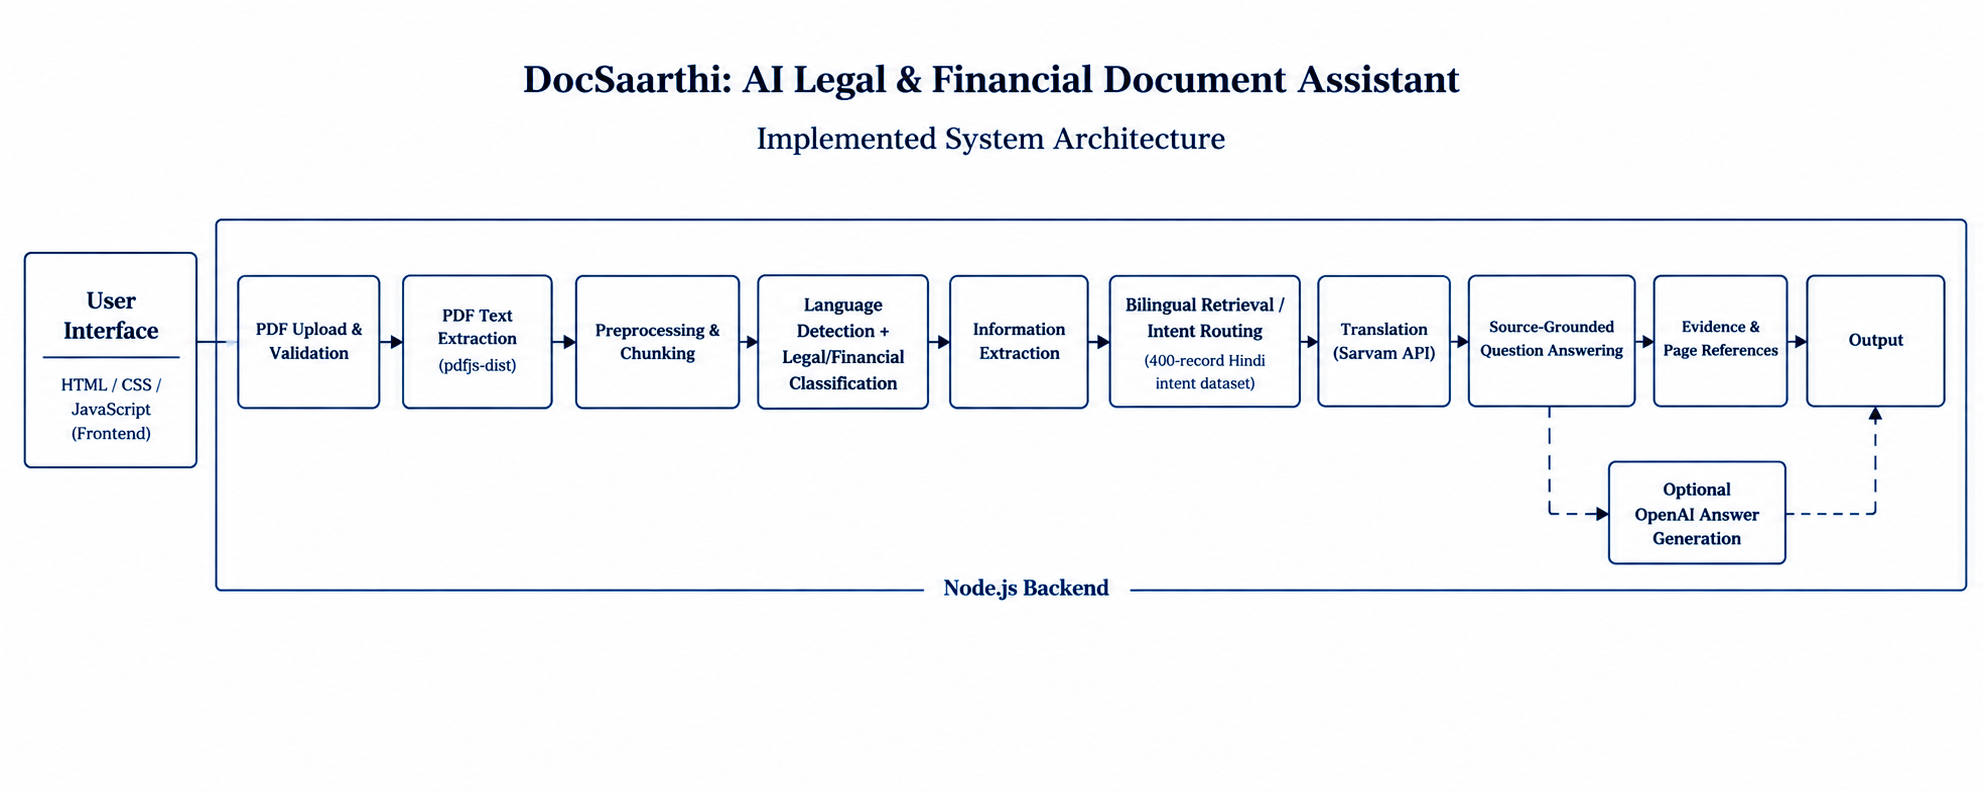
\includegraphics[width=0.95\textwidth]{figures/implemented_system_architecture.png.png}
\caption{Final Implemented System Architecture}
\label{fig:final_system_architecture}
\end{figure}

\section{Final End-to-End Workflow}
The user uploads a PDF; the server validates the file, extracts page-level text, detects language and document type, extracts important values, and builds searchable chunks. A user question is normalized and routed, relevant chunks are retrieved, an answer is formed only from those chunks, and the response includes page-linked evidence. Translation is performed on demand while the original PDF remains authoritative.

\section{Final System Implementation}
The implementation uses HTML, CSS, and JavaScript on the frontend; Node.js and Express on the backend; \texttt{pdfjs-dist} for extraction; local rule and lexical services for analysis and retrieval; and a 400-record Hindi dataset for intent signals. An offline English-Hindi parallel dataset supports known translations. OpenAI use is optional and controlled through configuration.

\section{Final Results}
The final build passes all 18 automated tests. On the eight-document labelled holdout, the system correctly classified all documents and detected both English and Hindi correctly. Source citations, page numbers, abstention, and critical-value preservation also passed their regression checks.

\section{Sample Outputs}
\begin{longtable}{|p{3.4cm}|p{4.3cm}|p{5.7cm}|}
\hline
\textbf{Input Scenario} & \textbf{Expected System Behavior} & \textbf{Verified Output Characteristic} \\
\hline
Hindi legal agreement with English termination query & Retrieve Hindi termination clause & Evidence contains the thirty-day clause and page 7 reference \\
\hline
English financial document with Hindi EMI query & Retrieve English repayment clause and answer in Hindi & Answer preserves the monthly EMI of ₹20,000 and cites the source excerpt \\
\hline
Question asking for absent PAN number & Do not infer an identifier & ``Information not found'' response, no source citation, grounded flag false \\
\hline
Financial translation request & Preserve protected values & Name, ₹5,00,000, 9.50\%, and 05/08/2029 remain unchanged \\
\hline
\end{longtable}

\section{Results Discussion}
The results show that a lightweight pipeline can provide useful, traceable assistance for controlled legal and financial samples. The strongest outcome is not the small-sample accuracy alone, but the combination of cross-language retrieval, source citations, value preservation, and safe abstention.

\section{Achievement of Project Objectives}
The prototype satisfies the principal objectives: PDF processing, Legal/Financial classification, bilingual interaction, structured information extraction, question answering from document evidence, page-level verification, and an accessible web interface. It also separates supporting datasets from authoritative document evidence.

\section{Limitations of the Final System}
The system does not yet support scanned PDFs without OCR, persistent multi-user storage, authentication, calibrated confidence, exhaustive legal or financial terminology, or production-scale evaluation. The translation memory can translate only supported content, and the in-memory repository loses documents when the server restarts.

\section*{Chapter Summary}
DocSaarthi delivers an operational end-to-end prototype with verified bilingual and grounding safeguards. The final results support academic demonstration while leaving clear work for production readiness.

\chapter{SDG, Sustainability, Safety and Societal Impact}
\label{chap:sdg_impact}

\section{Introduction}
DocSaarthi is intended to make complex legal and financial documents easier to explore without replacing qualified professional advice. This chapter connects the prototype to sustainable development, safety, ethics, and responsible use.

\section{SDG Alignment}
The project primarily supports United Nations Sustainable Development Goal 16, especially access to information and more inclusive institutions, by presenting document-grounded information in English and Hindi. It also supports SDG 10 by reducing language-based barriers and SDG 4 by helping users learn the terminology and structure of formal documents.

\section{Sustainability Considerations}
The lightweight rule-based and lexical pipeline runs on modest hardware and avoids mandatory large-model inference for every request. On-demand translation prevents unnecessary work. Digital document analysis can reduce repeated printing, although server operation, storage, and optional external AI services still consume energy and should be monitored in future deployments.

\section{Safety and Ethical Considerations}
Legal and financial content is sensitive and high impact. The system therefore keeps the uploaded PDF as the primary source, displays evidence, preserves important values, abstains when evidence is insufficient, and describes its output as assistance rather than professional advice. Synthetic evaluation data reduces privacy risk during testing.

\section{Societal Impact}
Potential benefits include improved access for Hindi-speaking users, faster identification of clauses and values, and better preparation before seeking professional help. Potential harms include over-reliance, incorrect interpretation, exposure of confidential documents, and unequal performance across document styles or languages.

\section{Responsible Use and Limitations}
Users must verify answers against the displayed source page and consult a lawyer, accountant, bank, or other qualified professional for consequential decisions. A production system requires encryption, user authentication, retention controls, access logs, consent, secure deletion, bias monitoring, and a clear incident-response process. The current prototype must not be used as an autonomous legal or financial decision maker.

\section*{Chapter Summary}
DocSaarthi can improve information accessibility when used as a transparent, source-linked assistant. Its benefits depend on privacy protection, careful limitation of claims, and continued human oversight.

\chapter{Project Management and Team Contribution}
\label{chap:project_management}

\section{Introduction}
The project was organized as a sequence of requirements, data, design, implementation, evaluation, and reporting milestones. Work was divided between Padmaja Shinde and Akshata Naik while key integration and validation tasks were completed jointly.

\section{Work Distribution}
\begin{table}[H]
\centering
\caption{Review 3 Work Distribution}
\begin{tabular}{|p{4cm}|p{4.5cm}|p{4.5cm}|}
\hline
\textbf{Area} & \textbf{Padmaja Shinde} & \textbf{Akshata Naik} \\
\hline
Core pipeline & PDF processing, preprocessing, chunking, retrieval, integration & Functional verification and bilingual workflow validation \\
\hline
Language support & Translation integration and intent handling & Translation fidelity and English/Hindi query testing \\
\hline
Quality & Backend debugging and source-grounding tests & Output, page evidence, classification, and unsupported-query tests \\
\hline
Documentation & Technical implementation content & Test evidence, results review, and presentation support \\
\hline
\end{tabular}
\end{table}

\section{Project Timeline and Milestones}
\begin{longtable}{|p{3cm}|p{5cm}|p{5cm}|}
\hline
\textbf{Phase} & \textbf{Milestone} & \textbf{Deliverable} \\
\hline
Review 1 & Problem definition, literature, dataset planning & Chapters 1--5 and proposed architecture \\
\hline
Review 2 & Prototype implementation and experimentation & Chapters 6--8, application modules, preliminary tests \\
\hline
Review 3 & Evaluation, error analysis, final results, impact, conclusion & Chapters 9--14, evidence appendices, final PDF and source archive \\
\hline
\end{longtable}

\section{Team Coordination}
The team used task-based ownership, shared review of interfaces between modules, and joint end-to-end testing. Findings from testing were converted into implementation changes and regression cases so that fixes could be verified after later edits.

\section{Testing and Quality Assurance}
Quality assurance includes automated unit and integration tests, an eight-document bilingual holdout, source-excerpt checks, value-preservation checks, and manual inspection of representative outputs. The complete automated suite was rerun for Review 3 and passed 18/18 tests.

\section{Version / Progress Tracking}
Source code and report material are maintained as version-controlled project files. Progress is tracked through implementation modules, test scripts, generated evaluation samples, and successive Review 1, Review 2, and Review 3 report chapters. Sensitive configuration values are separated from source through environment settings.

\section{Individual Contribution Summary}
Padmaja's primary contribution is the core document and NLP processing pipeline. Akshata's primary contribution is bilingual interaction, validation, testing, and system-level verification. Both members contributed to debugging, integration, documentation, and the final evaluation narrative. Detailed evidence is provided in Chapter 8 and Appendix E.

\section*{Chapter Summary}
The staged plan and complementary team roles enabled the project to progress from design to a tested final prototype. Traceable tests and artifacts provide evidence for the reported contributions.

\chapter{Conclusion and Future Scope}
\label{chap:conclusion}

\section{Introduction}
This chapter concludes the DocSaarthi project by summarizing the implemented outcome, major findings, current limitations, and practical directions for extension.

\section{Project Conclusion}
DocSaarthi demonstrates an end-to-end bilingual assistant for text-based legal and financial PDFs. It integrates page-level extraction, language and domain detection, structured information extraction, searchable evidence chunks, cross-language question handling, translation, grounded answers, and citations in a web application.

\section{Key Findings}
Page-linked chunking improves traceability; preserving dates, names, percentages, and currency values is essential for trustworthy bilingual output; intent data must be kept separate from document evidence; and explicit abstention is safer than forcing an answer. On the controlled Review 3 evaluation, all 18 tests passed and all eight holdout documents were correctly classified with correct language detection.

\section{Project Limitations}
The benchmark is synthetic and too small for general accuracy claims. The system lacks OCR for scanned pages, durable encrypted storage, authentication, calibrated probabilistic confidence, large-scale retrieval evaluation, and formal external human evaluation. Coverage of languages and document types is limited, and the local translation memory cannot translate arbitrary unseen passages.

\section{Future Scope}
Future work should include licensed real-world evaluation data, OCR with layout preservation, multilingual embeddings or a vector index, calibrated classification, retrieval ranking experiments, secure user-scoped storage, authentication and audit logs, formal human evaluation, support for additional Indian languages, and deployment monitoring. A carefully evaluated domain model may be introduced only after representative data and privacy controls are available.

\section*{Chapter Summary}
The project meets its academic goal by delivering a functional, transparent, and testable prototype. Its strongest foundation is source grounding; future work should preserve that principle while improving scale, coverage, privacy, and measured quality.



%================ References =================
\bibliographystyle{ieeetr}
\bibliography{references}

%================ Appendix ===================
\appendix
\begin{appendices}
%%%%%%%%%%%%%%%%%%%%%%%%%%%%%%%%%%%%%%%%%%%%%%%%%%%%%%%%%%%%%%
\chapter{AI Compliance}

%%%%%%%%%%%%%%%%%%%%%%%%%%%%%%%%%%%%%%%%%%%%%%%%%%%%%%%%%%%%%%

\section{AI Tools Used}

The following Artificial Intelligence (AI) tools were used during the preparation of this micro project report:

\begin{itemize}
    \item ChatGPT (OpenAI)
    \item Codex (OpenAI)
    \item Claude AI (Anthropic)
\end{itemize}

These tools were used only as academic writing assistants to improve the quality and presentation of the report.

%%%%%%%%%%%%%%%%%%%%%%%%%%%%%%%%%%%%%%%%%%%%%%%%%%%%%%%%%%%%%%

\section{Nature of Assistance}

The AI tools were used for the following purposes:

\begin{itemize}
    \item Improving grammar, sentence structure, and academic writing style.
    \item Assisting in the organization and formatting of the report in \LaTeX{} (Overleaf).
    \item Providing explanations of NLP concepts, machine learning models, and research methodologies.
    \item Assisting in drafting sections of the report based on the project requirements.
    \item Helping summarize and understand selected research papers.
    \item Suggesting suitable datasets, preprocessing techniques, feature representation methods, and evaluation metrics relevant to the proposed NLP system.
    \item Assisting in generating diagrams, workflow descriptions, and documentation while ensuring consistency throughout the report.
    \item Assisting in reorganizing the Review 3 report, preparing evaluation tables from verified test output, and checking the compiled PDF layout.
\end{itemize}

The final selection of content, project design, implementation decisions, and verification of technical information were carried out by the author.

%%%%%%%%%%%%%%%%%%%%%%%%%%%%%%%%%%%%%%%%%%%%%%%%%%%%%%%%%%%%%%

\section{Ethical Compliance Statement}

I hereby declare that Artificial Intelligence (AI) tools were used only to assist in academic writing, report organization, language improvement, and understanding technical concepts. All project ideas, implementation decisions, dataset preparation, literature review, analysis, and final conclusions were carefully reviewed and verified by me. Proper credit has been given wherever external sources were consulted, and all research papers have been cited appropriately. I affirm that this report represents my own academic work and complies with the ethical guidelines prescribed by the institution regarding the responsible use of AI-assisted tools.

\chapter{Plagiarism Report}

The plagiarism report generated for the Stage-1 Micro Project is attached in the following pages.

\IfFileExists{appendices/PDF/Similarity_report.pdf}{
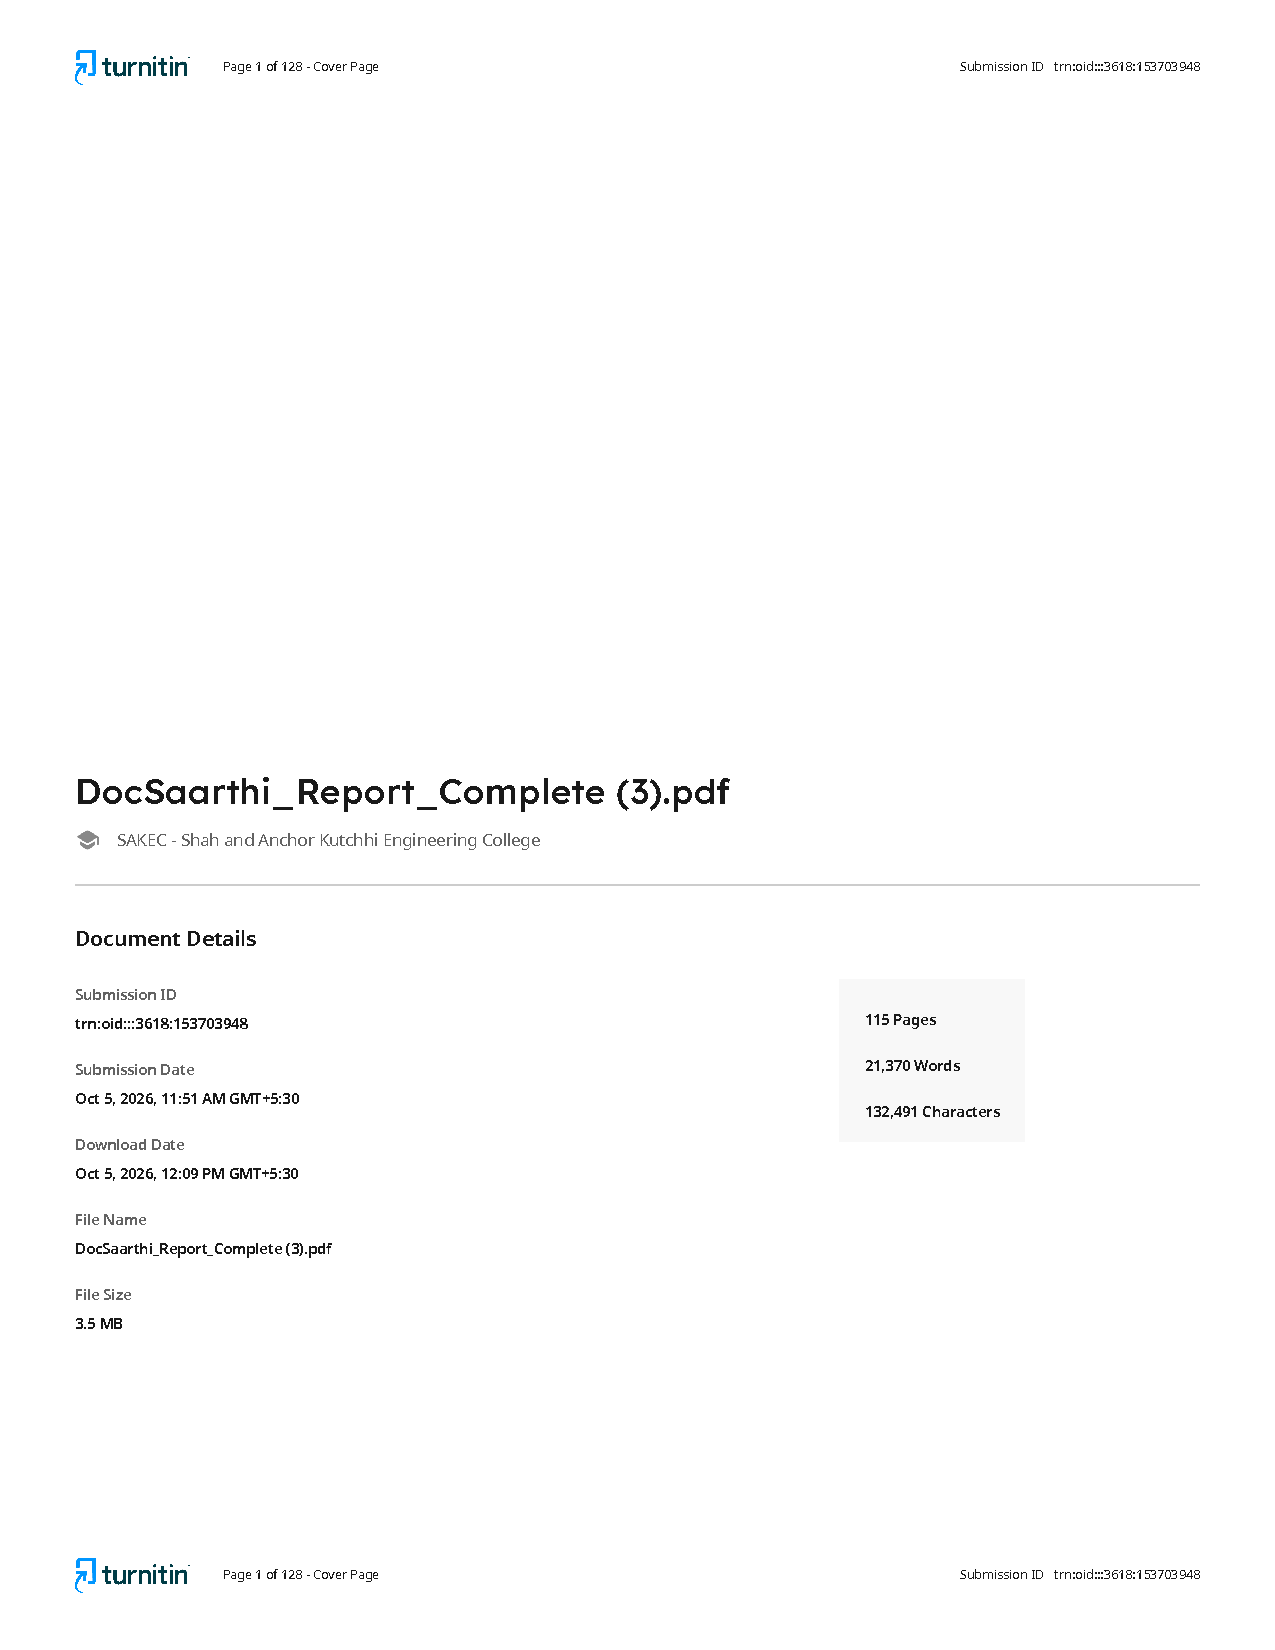
\includepdf[
    pages=-,
    pagecommand={},
    scale=0.9
]{appendices/PDF/Similarity_report.pdf}
}{
\textbf{[Missing file: \texttt{appendices/PDF/plagiarism\_report.pdf} was not found in the project folder. Add the actual plagiarism-check PDF for this submission here before final submission.]}
}
\chapter{AI Writing Report}
\label{app:ai_writing}
\IfFileExists{appendices/PDF/AI_report.pdf}{
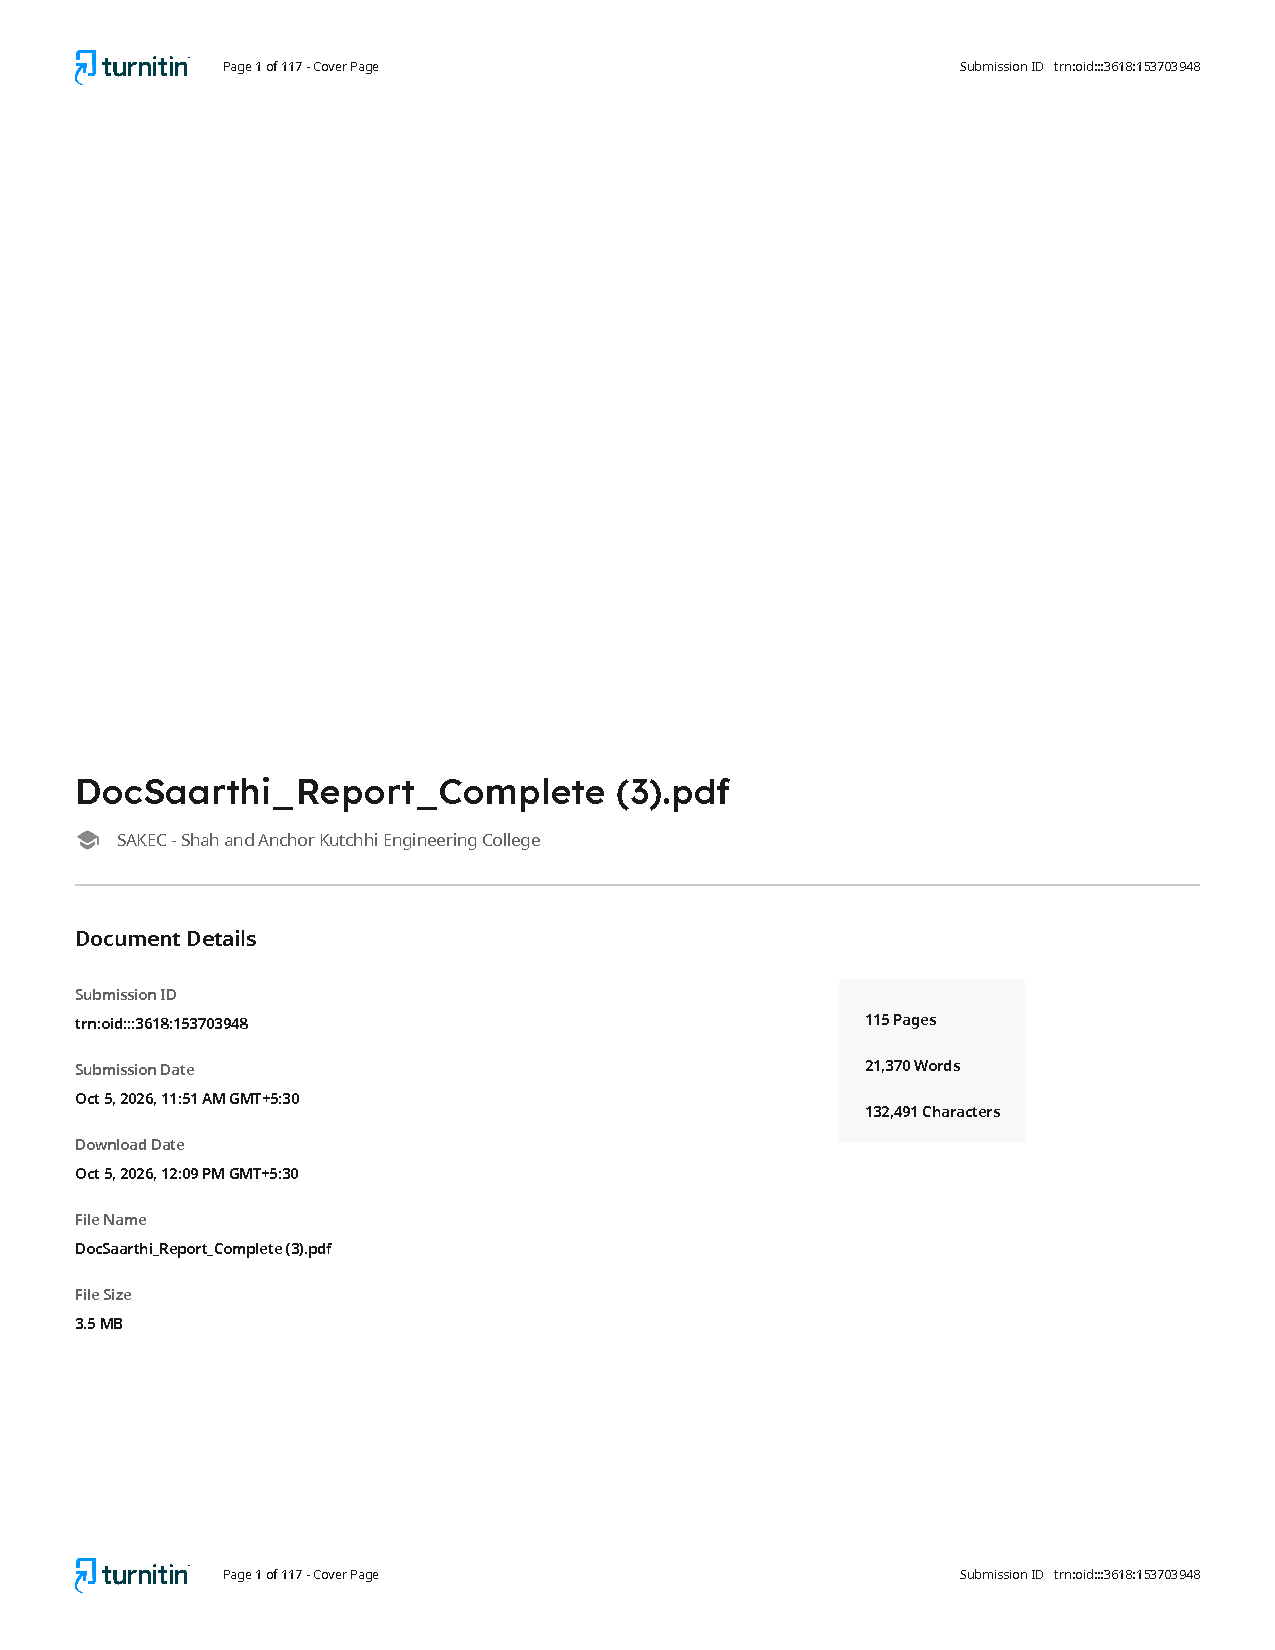
\includepdf[
  pages=-,
  pagecommand={\thispagestyle{plain}},
  scale=0.9
]{appendices/PDF/AI_report.pdf}
}{
\textbf{[Missing file: \texttt{appendices/PDF/ai\_writing\_report.pdf} was not found in the project folder. Add the actual AI-writing disclosure PDF here before final submission.]}
}
\chapter{Assessment Rubrics}
\label{app:evaluation_critera}
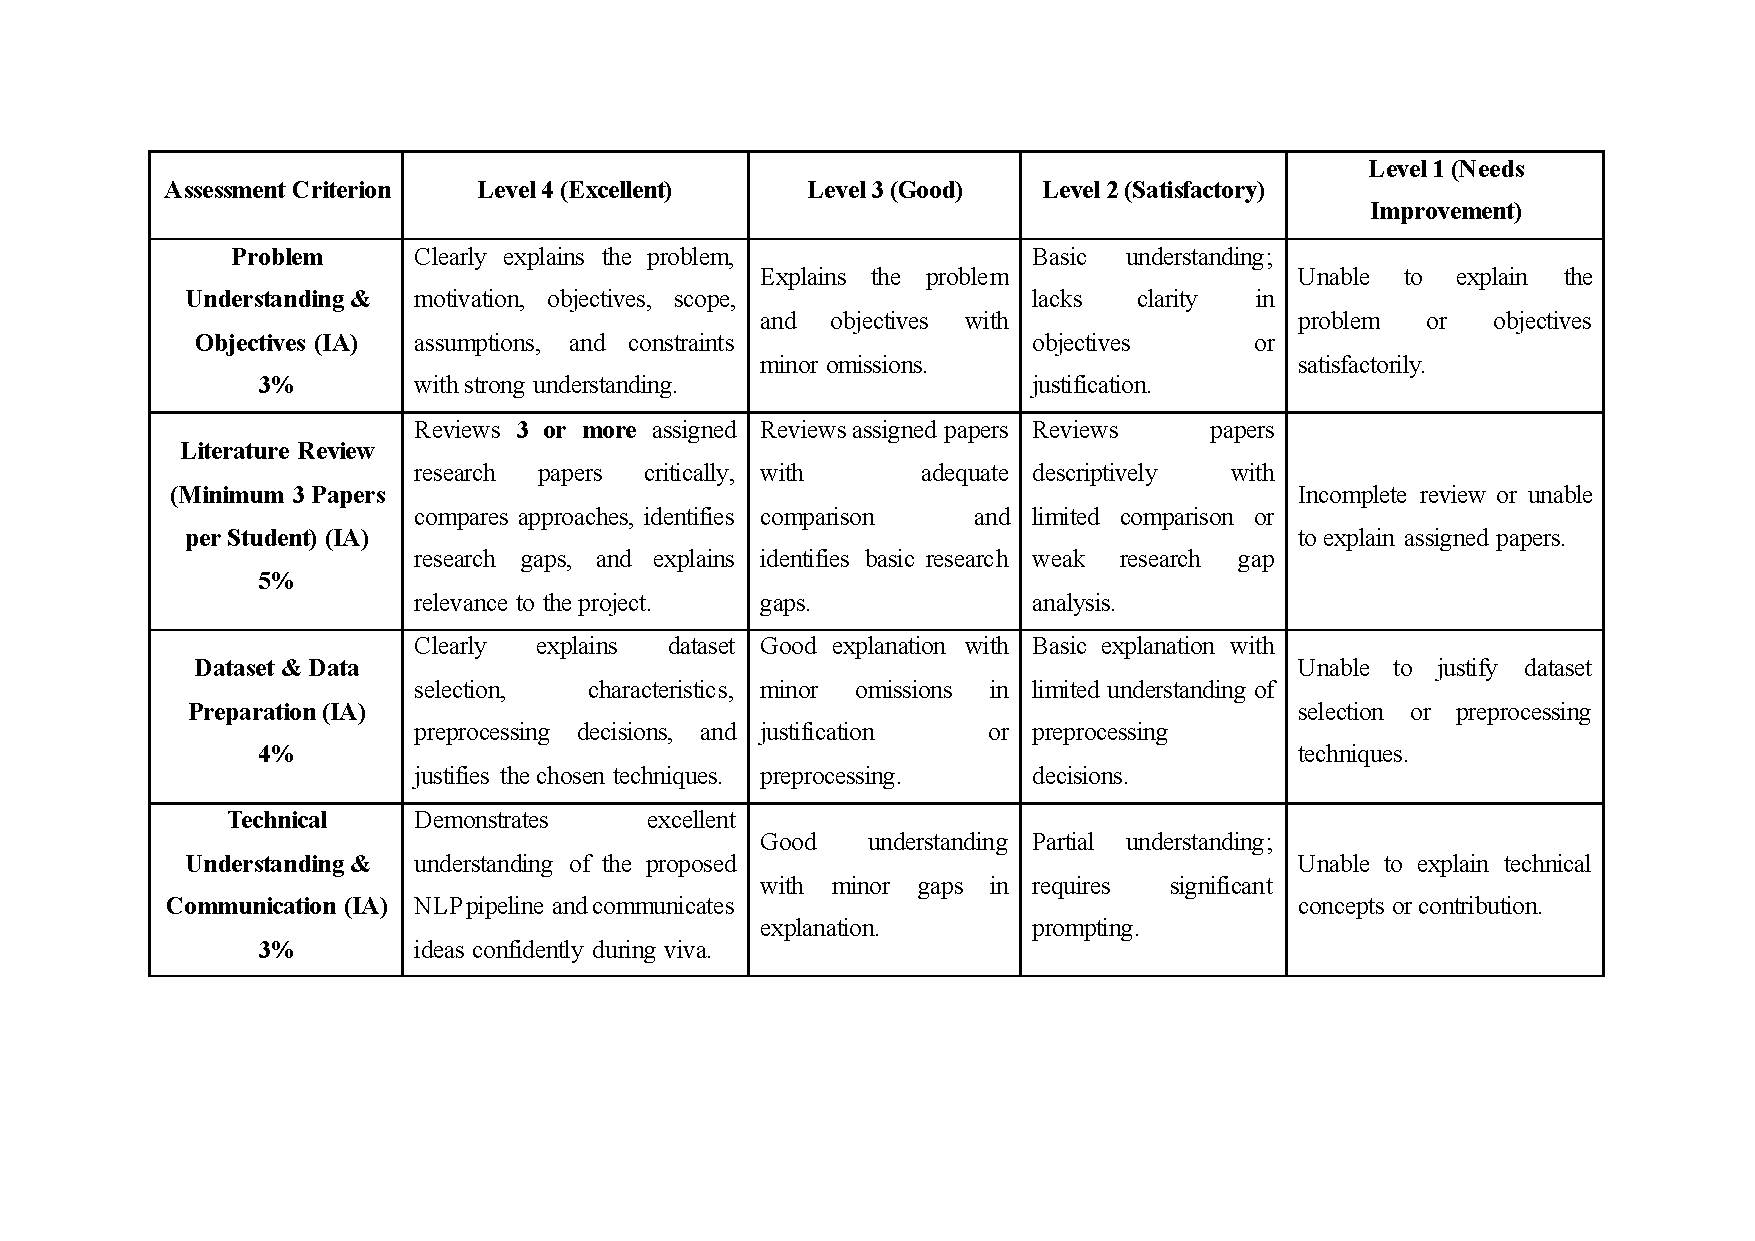
\includepdf[
  pages=-,
  angle=90,
  pagecommand={\thispagestyle{plain}},
  scale=0.9
]{appendices/PDF/evalution_crieria.pdf}
\chapter{Supporting Evidence}

\section{Dataset Samples}
The project dataset contains 400 Hindi intent records. The verified distribution is: Agreement 40, Payment 20, Court Proceeding 80, Confidentiality 40, General 60, Finance 100, Loan 20, Tax 20, and Insurance 20. Records are used for intent support only and not as document evidence.

\section{Preprocessing Examples}
Verified preprocessing cases include repair of sentence-breaking PDF line breaks, preservation of Devanagari combining marks, Unicode normalization, and page-linked evidence chunking. Original source text is retained for verification.

\section{Experimental Logs}
The final automated run reports 18 tests, 18 passes, and zero failures. The classifier evaluation reports eight labelled samples, 100\% classification accuracy, macro-F1 1.00, and 100\% language-detection accuracy. These results apply only to the controlled synthetic benchmark.

\section{Additional Results}
Additional validated behaviors include English-to-Hindi retrieval, Hindi-to-English retrieval, preservation of ₹ amounts, percentages, dates, and names, safe handling of unavailable translation, and abstention when a requested fact is absent.

\section{Individual Contribution Evidence}
Evidence includes source modules, test cases, evaluation scripts, bilingual sample PDFs, result logs, interface screenshots, and report chapters. Chapter 8 records task-level contributions and Chapter 13 summarizes Review 3 responsibilities.

\end{appendices}


\end{document}
